% !TEX root = arbeit.tex
\section{Theory} \label{sec:theory}

	NIM is a time-of-flight mass spectrometer consisting of an ion-source, a mass analyser and a detector. Fig.~\ref{fig:NIMSketch} shows a schema of the NIM ion-optical system. Gaseous particles enter the ion-source either through a closed source antechamber where they get thermalised or directly through an entrance slit. The measuring mode where the thermalised particles entering through the antechamber are analysed is called thermal mode (th-mode). The measuring mode where neutral particles are analysed, which enter the ionisation region directly is called neutral mode (n-mode) and the mode where ions are analysed is called ion mode (i-mode). The neutral particles are ionised by electron impact ionisation. A filament is heated to a temperature where it emits electrons. The electrons are accelerated up to an energy of about --70~eV. In the ionisation region, the electrons knock out electrons from the neutral gas generating positive ions. The ions are then accelerated to an energy of about 250~eV by applying a high voltage pulse on the extraction grid. NIM has a two-field ion source meaning that with the ion-optical lenses the ions are additionally accelerated and focused to compensate when the ions have different initial energies.
	\begin{figure}[h!]
		\centering
		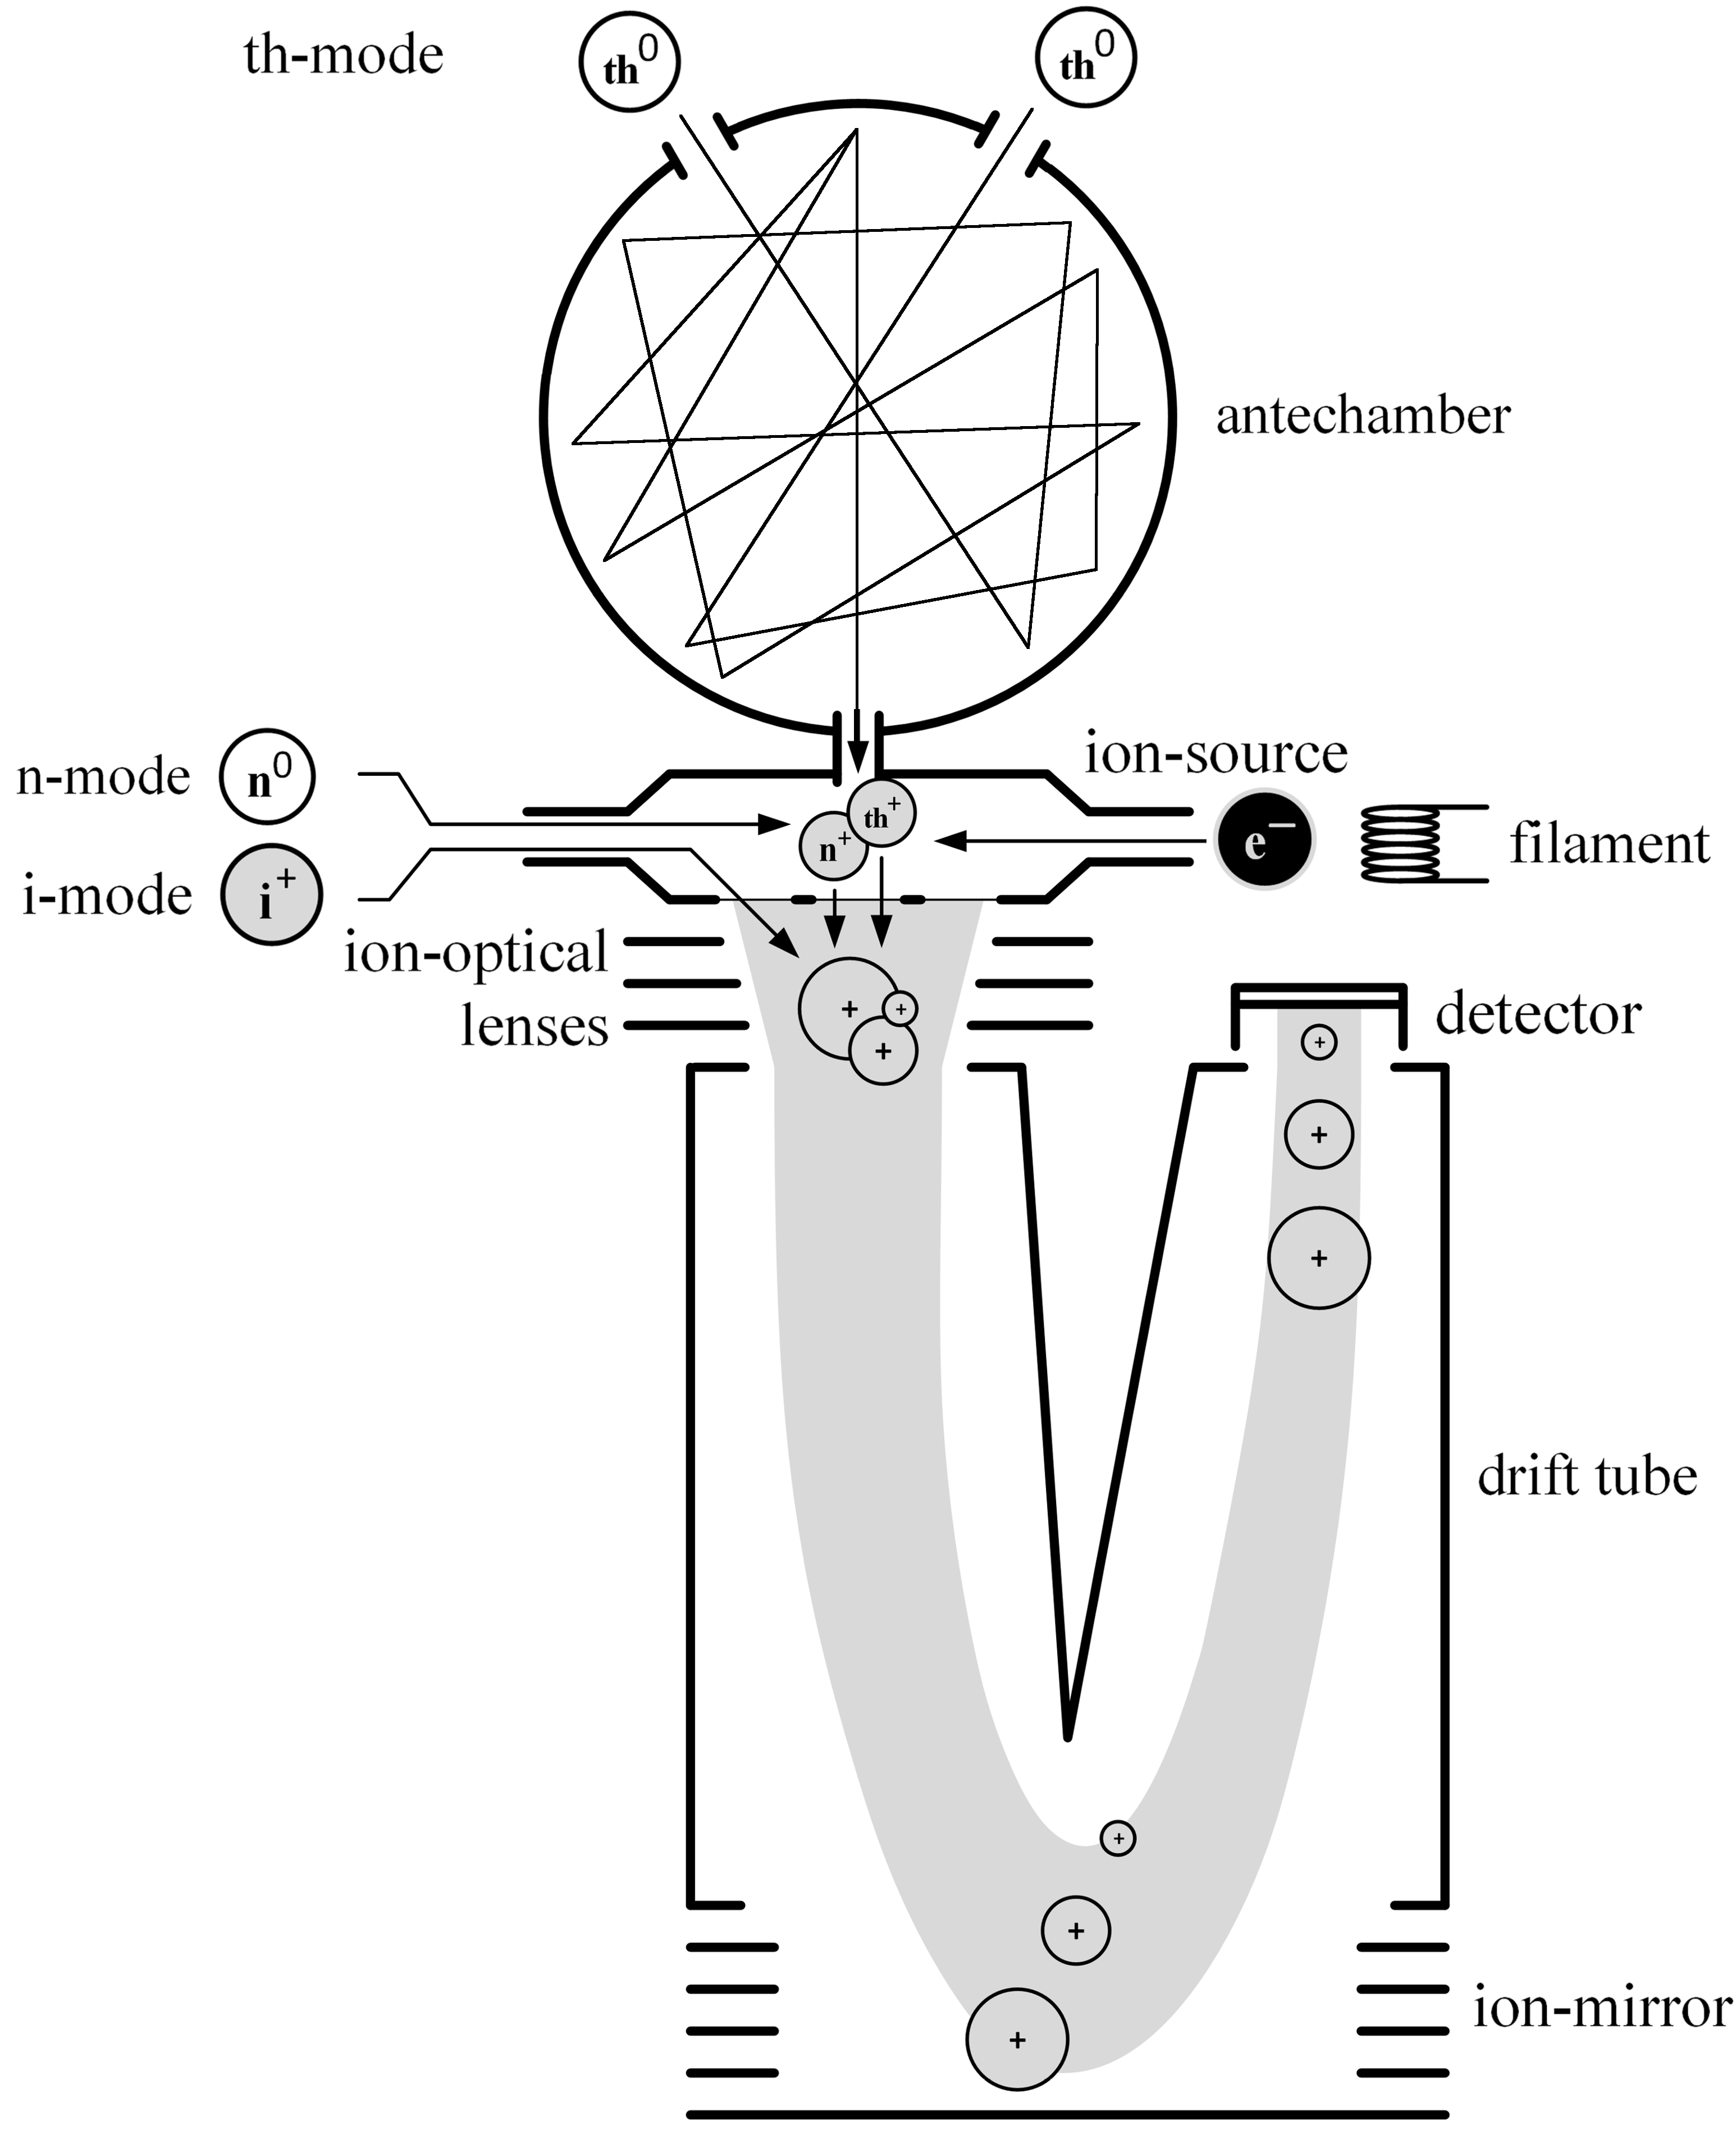
\includegraphics[width= 10cm]{Bilder/NIM_Sketch.png}
		\caption{Schematics of the NIM mass spectrometer. Adapted from \cite{Diss_Meyer}.}
		\label{fig:NIMSketch}
	\end{figure}
	Light species fly faster through the time-of-flight mass spectrometer than heavier ones resulting in a separation of the species by their mass. An ion-mirror is used to increase the flight distance and to refocus ions of the same species with different energies. The ions are detected with a Multi-Channel-Plate (MCP) detector.\\
	This chapter gives an overview from the theoretical perspective over the different subunits of the NIM ion-optical system.	Chap.~\ref{sec:Exp} shows test results of the different subunits and performance tests of the NIM Prototype, the NIM Proto~Flight~Model (PFM) and the Flight~Spare (FS) models.
		
%---------------------------------------------------------------------------------------
	\subsection{Mass Resolution}\label{chap:massRes}
	The generated ions in the ion-source are trapped in the centre by the potentials of the electrodes and the electron beam. The ions are extracted into the analysis section by a high voltage pulse applied onto the extraction grid. All ions are accelerated to the same energy $W$:
	\begin{equation}
		W = \int_{0}^{s_0}q E_s ds =  \frac{q U_0}{2}
		\label{eq:WIonPulse}
	\end{equation}
	With $s_0$ the distance from the centre of the ion-source to the extraction grid corresponding to half the height of the ion-source. $q$ is the particle charge, $E_s$ is the applied electric extraction field strength induced by the voltage $U_0$ applied on the extraction grid. The nominal starting position of the ions is in the centre of the ion-source. Therefore, they have the kinetic energy $q U_0/2$ when reaching the extraction grid:
	\begin{equation}
		\frac{q U_0}{2} = \frac{1}{2}m v^2
	\end{equation}
	With $m$ and $v$ the mass and velocity of the ion. Rearranging this formula results in:
	\begin{equation}
		\frac{m}{q} = U_0\frac{t^2}{D^2}
		\label{eq:m/q}
	\end{equation}
	With $t$ the time of flight and $D$ the flight distance from the extraction grid to the detector. $U_0$ and $D^2$ are merged into one constant $C$ resulting in:
	\begin{equation}
		\frac{m}{q} = C(t-t_0)^2
		\label{eq:mass_Calib}
	\end{equation}
	$t_0$ corresponds to a time offset between the start of the mass axis and the time axis. The two calibration constants $C$ and $t_0$ are determined by at least knowing two species in the mass spectrum. The correctness of the mass scale can be verified by checking the other mass peaks in the mass spectrum, which all have to be on integer masses, ignoring the small deviations for now. The mass is therefore proportional to $t^2$:
	\begin{equation}
		m = c\cdot t^2
		\label{eq:mt2}
	\end{equation}
	The derivative is:
	\begin{align}
		\frac{dm}{dt} &= 2~ct\\
		dm &= 2~ct\cdot dt
		\label{eq:dm}
	\end{align}
	Dividing Eq.~\eqref{eq:mt2} through Eq.~\eqref{eq:dm} results in:
	\begin{align}
		\frac{m}{dm} &= \frac{ct^2}{2~ct\cdot dt}\\
		\frac{m}{dm} &= \frac{t}{2~dt} = \frac{\mu}{2\cdot FWHM}
		\label{eq:massRes}
	\end{align}
	With $\mu$ the centre of the mass peak in the time domain and $FWHM$ is the full width at half maximum of the mass peak \cite{LecNot_Wurz2017}.\\
	
	In the following section, the different contributions affecting the mass resolution are analysed. The focus is on the contributions originating from the ion source because they have the biggest impact on the mass resolution of the instrument.\\
	The total time spread $dt_i$ of the signal of a particle species $i$ at the detector is:
	\begin{equation}
		dt_i = \sqrt{\sum_{k} dt_k^2} = \sqrt{dt_D^2 + dt_{ADC}^2 + dt_{th}^2 + dt_{s}^2 + dt_{tfall}^2}
		\label{eq:dti}
	\end{equation}
	With the different contributions $dt_k$ assumed to be independent from each other. When an ion hits the detector, it generates a charge pulse with pulse width $dt_D$. For the NIM detector, the pulse width is $\sim$~0.7~ns. The generated pulse is converted into a digital signal with an analogue-to-digital converter (ADC). The ADC used in the laboratory has a sampling rate of 4~GHz resulting in a time resolution $dt_{ADC}$ of 0.25~ns. The flight ADC has a maximal sampling rate of 2~GHz corresponding to a time resolution of 0.5~ns. The contribution to the time spread by the ion-mirror is small compared to the other effects and can therefore be neglected.\\ % About 1 decade later than the other effects (in mass resolution).

	The time spreads resulting from the thermal energy of the ions $dt_{th}$, from the different start positions of the ions within the ionisation region $dt_s$ and from the fall time of the high voltage pulse $dt_{tfall}$ are coupled because they all affect the energy deviation from the nominal energy (Eq.~\eqref{eq:WIonPulse}) of the ions. Initially, the ions in the ion-source have thermal energy $W_{th}$:
	\begin{equation}
		W_{th} = \frac{3}{2}\cdot k_B \cdot T
	\end{equation}
	With $k_B$ the Boltzmann constant and $T$ the temperature. The thermal energy leads to an initial velocity distribution of the ions with a mean velocity of $v_{init}$ (Fig.~\ref{fig:thISStartPosThermEn} top panel). Ions number 1 and 3 have the same thermal energy but one is directed towards the extraction grid where the other one is directed towards the backplane. When a high voltage pulse is applied on the extraction grid, ion number 3 has to be turned around. The time difference between ions 1 and 3 is called turn-around time. At a certain point in time, ion 3 will overtake ions with less energy (ion 2). The turn-around time cannot be corrected with the ion optics. The only option to reduce the turn-around time would be to cool the ions, which is not possible for a space instrument.\\
	The total energy $W$ the ions get in the ionisation region is:
	\begin{equation}
		W = \int_{s_{init}}^{s_0} q\cdot E(t)\cdot ds
		\label{eq:WionsISposEt}
	\end{equation}

	\begin{figure}[H] % space and velocity deviation.
		\centering
		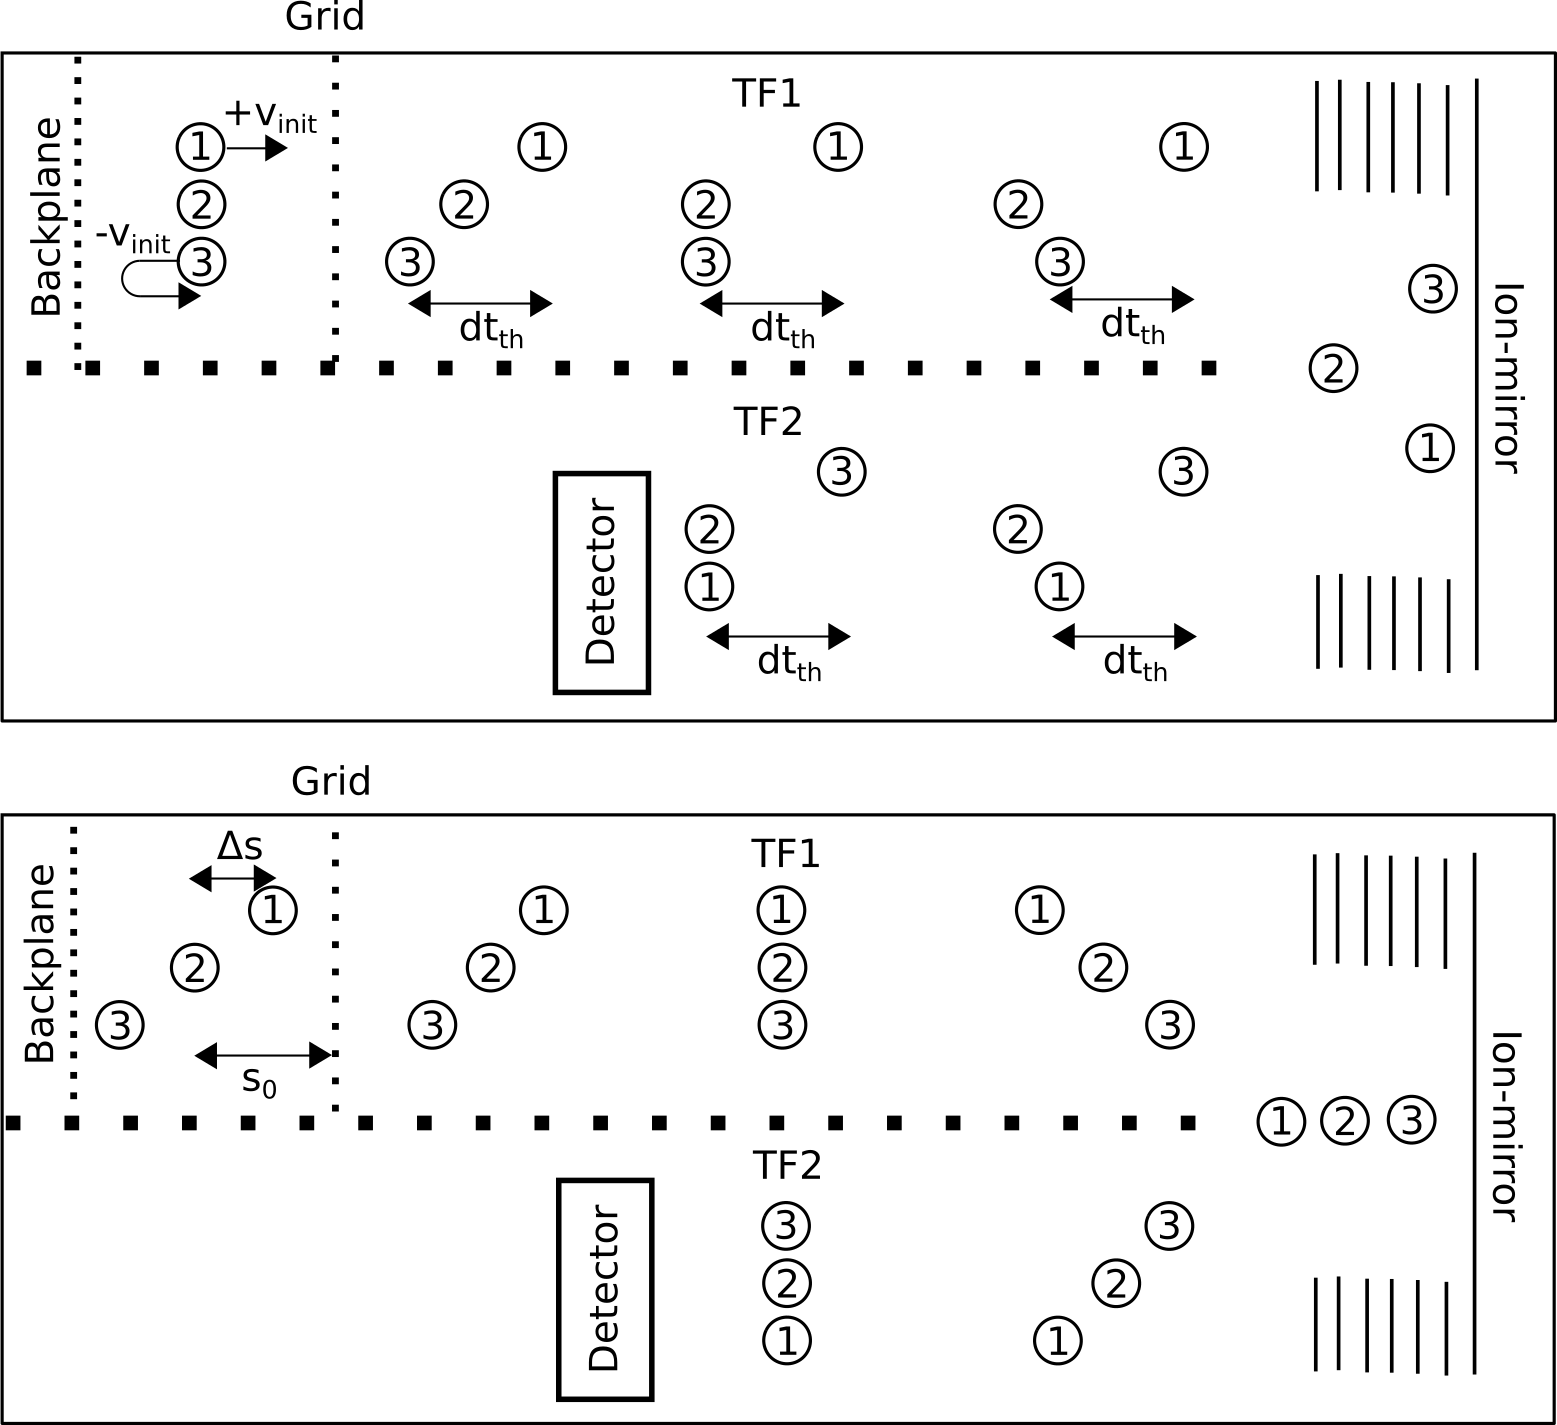
\includegraphics[width= .9\textwidth]{Bilder/ISStartPosThermEn.png}
		\caption{Flight path of ions with different thermal energy (top panel) and start positions (lower panel). $v_{init}$ is the initial velocity of the ions and $dt_{th}$ the turn-around time. TF1 and TF2 are the locations of the first and second time focus respectively.}
		\label{fig:thISStartPosThermEn}
	\end{figure}

	With $s_{init}$ the initial position of the ions, $s_0$ the distance from the centre of the ionisation region to the acceleration grid, $q$ the particle charge and $E(t)$ the electric field strength depending on the time $t$. When the ions start at different positions in the ionisation region $s_{init}$, they receive a different amount of energy because their flight distance in the acceleration field is different (Fig.~\ref{fig:thISStartPosThermEn} lower panel). At a certain distance on the flight path, ions with higher energy will overtake ions with lower energy. The time spread induced by the different start positions of the ions is $dt_{s}$. With a two-field ion source, like NIM, $dt_s$ can be minimised at the first time focusing point TF1. With an ion-mirror ions with an energy spread up to 10~\% are refocused. Ions with higher energy penetrate deeper into the ion-mirror resulting in a longer flight path of the higher energetic ions. The best position for the detector is when all ions with different energies are at the same position, which is at the time focus of the ion mirror TF2.\\
	% This point is at around $2\cdot s_0$
	
	\begin{figure}[H]
		\begin{subfigure}{0.5\textwidth}
			\centering
			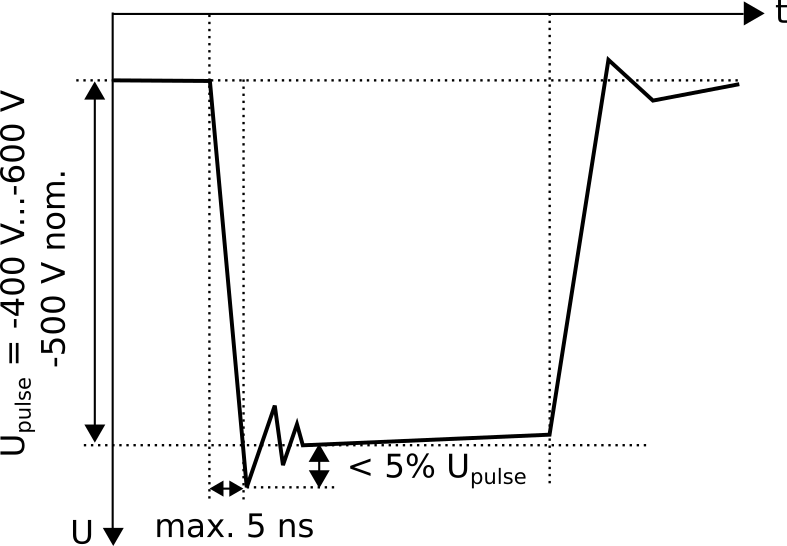
\includegraphics[width=\textwidth]{Bilder/PulserShapeTheoAna.png}
			\caption{}
			\label{subfig:theoPulseShape}
		\end{subfigure}
		\begin{subfigure}{0.5\textwidth}
			\centering
			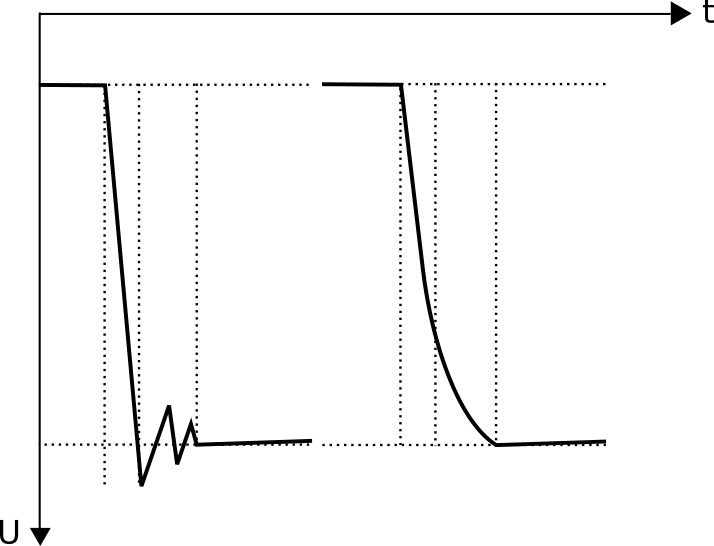
\includegraphics[width=.9\textwidth]{Bilder/PulserFallTimeShapes.png}
			\caption{}
			\label{subfig.PulserFallTimeShapes}
		\end{subfigure}
		\caption{a) Shape of a realistic high voltage pulse applied on the extraction grid. b) Two different possible shapes of the falling edge of the high voltage pulse.}
		\label{fig:theoPulseShape}
	\end{figure}
	\begin{figure}[h!] % Electric field vs. position s
		\centering
		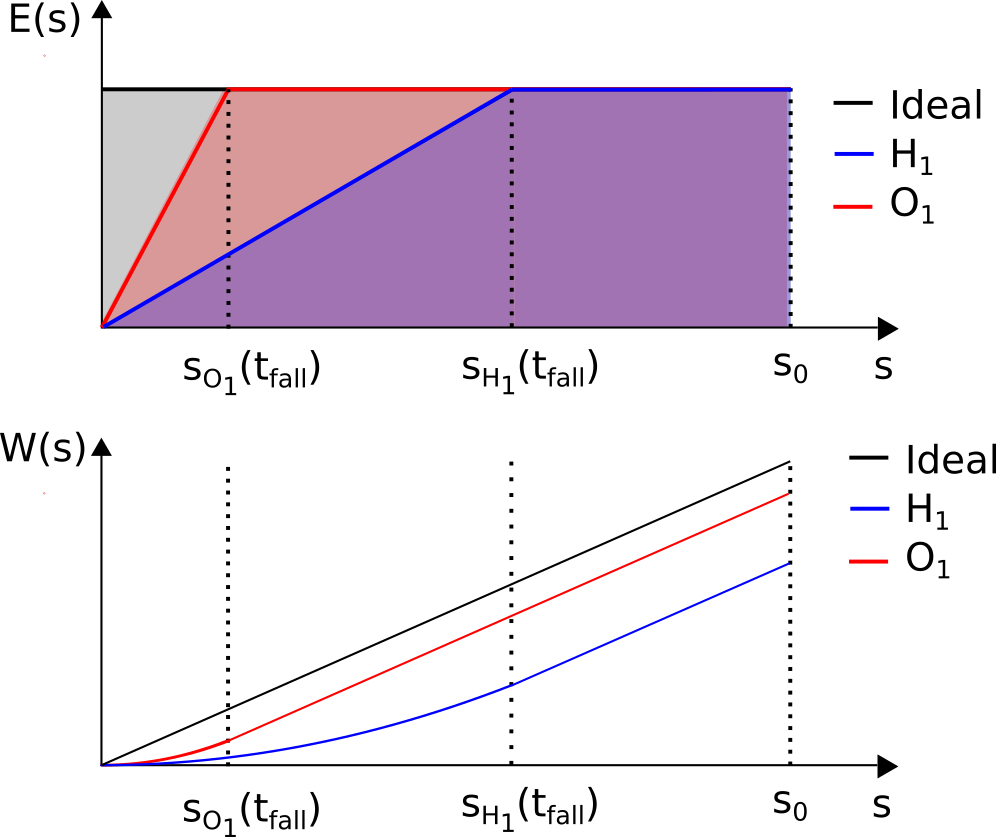
\includegraphics[width= 0.7\textwidth]{Bilder/PulsInt.png}
		\caption{Top panel: Electric field $E(s)$ an ion experiences, as a function of the distance between the centre of the ionisation region and the extraction grid $s_0$ for two hydrogen (H\textsubscript{1}) and oxygen (O\textsubscript{1}). $s_i(t_{fall})$ is the position of the corresponding species at the fall time $t_{fall}$. Lower panel: Energy $W(s)$ of the ions as a function of their position.}
		\label{fig:PulsInt}
	\end{figure}
	
	Ideally, the shape of the extraction pulse is a rectangle. Fig.~\ref{subfig:theoPulseShape}) shows the shape of a realistic extraction pulse. The pulse needs the time $t_{fall}$ to build up the extraction potential on the extraction grid. Fig.~\ref{fig:PulsInt}~top panel shows the changing electric field as a function of the position for atomic hydrogen (H\textsubscript{1}) and oxygen (O\textsubscript{1}) in case when these two species start at the same position. The total energy $W$ of the ions at the exit of the extraction region corresponds to the area under the curves. The energy as a function of the flight distance $s$ in the ionisation region is plotted on the bottom panel of Fig.~\ref{fig:PulsInt}. Hydrogen is lighter than oxygen and therefore, it leaves the ionisation region earlier. This results in a smaller amount of energy for hydrogen than for oxygen. The shorter the fall time of the high~voltage pulse is, the smaller is the energy difference because it shifts the position of the ions at the fall time $s_i(t_{fall})$ towards zero. When looking at the shape of the falling edge of the pulse (Fig.~\ref{subfig.PulserFallTimeShapes}), it is more important to have a small fall time with an overshoot than a pulse slowly converging to the maximum because the resulting energy deviation in the first case is much smaller than in the second.\\
	
	In the following section the influence of the fall time of the high~voltage pulse $t_{fall}$ in combination with the longitudinal spacial spread $\Delta s$ of the ions in the ionisation region and the thermal energy of the ions on the mass resolution is analysed. To investigate the impact of these effects, this model does not include any focusing lenses and has no ion-mirror.\\
	The derivation of the equation of motion is based on \cite{Diss_Abplanalp}. The electric field $E(t)$ in the ionisation region is approximated with a linear function during the fall time $t_{fall}$ and as a constant during the rest of the time:
	\begin{equation}
		E(t) =
		\begin{cases}
			E_1\cdot\frac{t}{t_{fall}},& (0\leq t\leq t_{fall})\\
			E_1,& t_{fall} < t
		\end{cases}
	\label{eq:PulseEt}
	\end{equation}
	$E_1$ is the electric field strength when the high voltage pulse is fully applied:
	\begin{equation}
		E_1 = \frac{U_0}{2\cdot s_0}
	\end{equation}
	With $U_0$ the voltage on the extraction grid. The equation of motion for the ions during the fall time is:
	\begin{equation}
		a_{fall}(t\leq t_{fall}) = \frac{q\cdot E_1}{m\cdot t_{fall}}\cdot t
		\label{eq:afall}
	\end{equation}
	With $a_{fall}$ the acceleration of the ions and $m$ the ion mass. The velocity of the ions $v_{fall}$ is:
	\begin{equation}
		v_{fall}(t\leq t_{fall}) = \frac{q\cdot E_1}{2\cdot m\cdot t_{fall}}\cdot t^2 + v_{init}\label{eq:vfall}
	\end{equation}
	With $v_{init}$ the initial velocity of the ions before applying the extraction pulse. $v_{init}$ originates from the ion's thermal energy. The position of the ions $s_{fall}$ at the time $t$ is:
	\begin{equation}
		s_{fall}(t\leq t_{fall}) = \frac{q\cdot E_1}{6\cdot m\cdot t_{fall}}\cdot t^3 + v_{init}\cdot t + s_{init}
		\label{eq:sfall}
	\end{equation}
	With $s_{init}$ the initial position of the ions. When the high voltage pulse is fully applied and the ions did not reach the extraction grid until that time, the acceleration of the ions $a_{p}$ is:
	\begin{equation}
		a_{p}(t > t_{fall}) = \frac{q\cdot E_1}{m}
		\label{eq:ap}
	\end{equation}
	The velocity $v_{p}$ is:
	\begin{equation}
		v_{p}(t > t_{fall}) = \frac{q\cdot E_1}{m}(t-t_{fall}) + v_{fall}(t_{fall})
		\label{eq:vp}
	\end{equation}
	With $v_{fall}(t_{fall})$ the velocity of the ions at the time $t_{fall}$. The position $s_{p}$ is:
	\begin{equation}
		s_{p}(t > t_{fall}) = \frac{q\cdot E_1}{2\cdot m}(t-t_{fall})^2 + v_{fall}(t_{fall})(t-t_{fall}) + s_{fall}(t_{fall})
		\label{eq:sp}
	\end{equation}
	With $s_{fall}(t_{fall})$ the position of the ions at the time $s_{fall}$. When the ions leave the ionisation region before full high voltage is applied on the extraction grid, the time they spend in the ionisation region $t_{IS}$ is calculated by setting $s_{fall}=s_0$ and solving the cubic Eq.~\eqref{eq:sfall} for $t$. The velocity $v_{Grid}$ of the ions at the extraction grid is determined by inserting $t_{IS}$ in Eq.~\eqref{eq:vfall}.\\
	When the ions leave the ionisation region after the high voltage is fully applied, the time they spend in the ionisation region $t_{IS}$ is calculated by setting $s_{p}=s_0$ and solving Eq.~\eqref{eq:sp} for $t$. The velocity $v_{Grid}$ of the ions at the extraction grid is determined by inserting $t_{IS}$ in Eq.~\eqref{eq:vp}. The total flight time of the ions in this model is:
	\begin{equation}
		t_{TOF} = t_{IS} + t_D
	\end{equation}
	With $t_{D}$ the time of flight the ions need for the distance between the extraction grid and the detector. The mass resolution is calculated according to Eq.~\eqref{eq:massRes}. To have a measure for the impact of the fall time on the different masses, the deviation $R$ of the mass resolution of ions with a mass/charge ratio $i$ relative to the mass resolution of ions with a mass/charge ratio of 200 is calculated:
	\begin{equation}
		R = 1 - \frac{m_i/\Delta m_i}{m_{200}/\Delta m_{200}}
	\end{equation}
	\begin{figure}[H] % Fall time plots
		\centering
		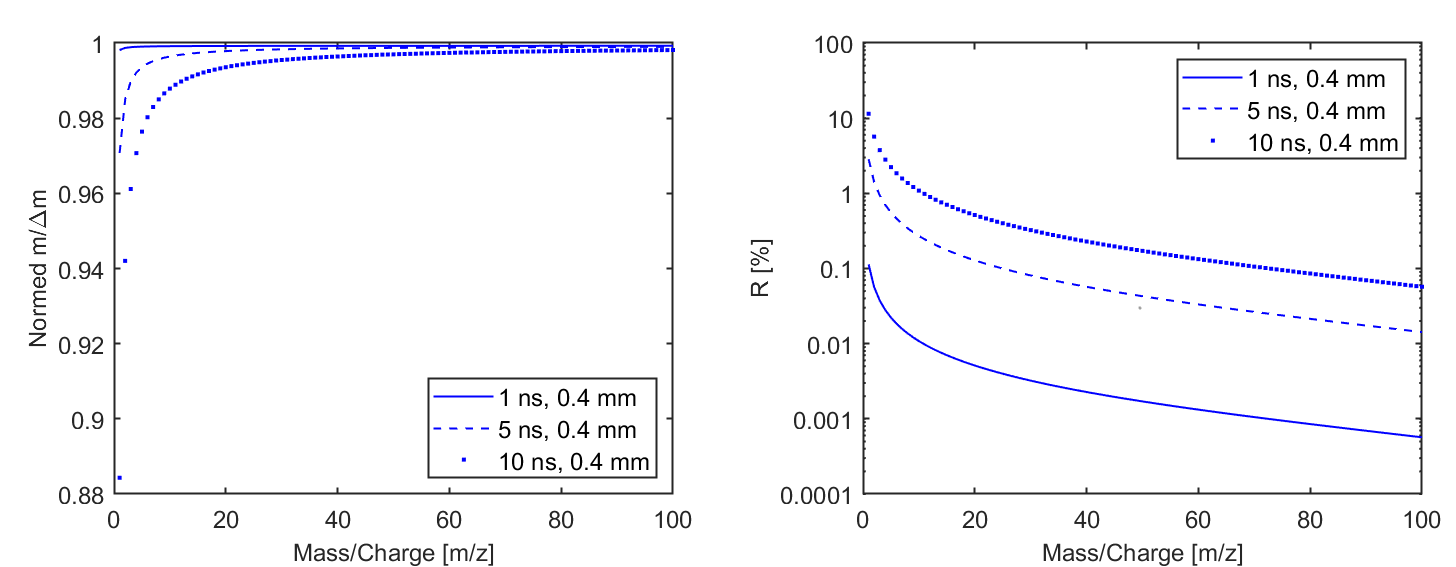
\includegraphics[width=\textwidth]{Bilder/PulseSimMassRes_Norm.png}
		\caption{Left: Calculated mass resolution as a function of the mass/charge ratio of the ions for three different fall times of the extraction pulse. Right: relative deviation of the mass resolution from the mass resolution plateau as a function of the mass/charge ratio.}
		\label{fig:Simtfall}
	\end{figure}
	\begin{figure}[h!] % Lab WLE measurement
		\centering
		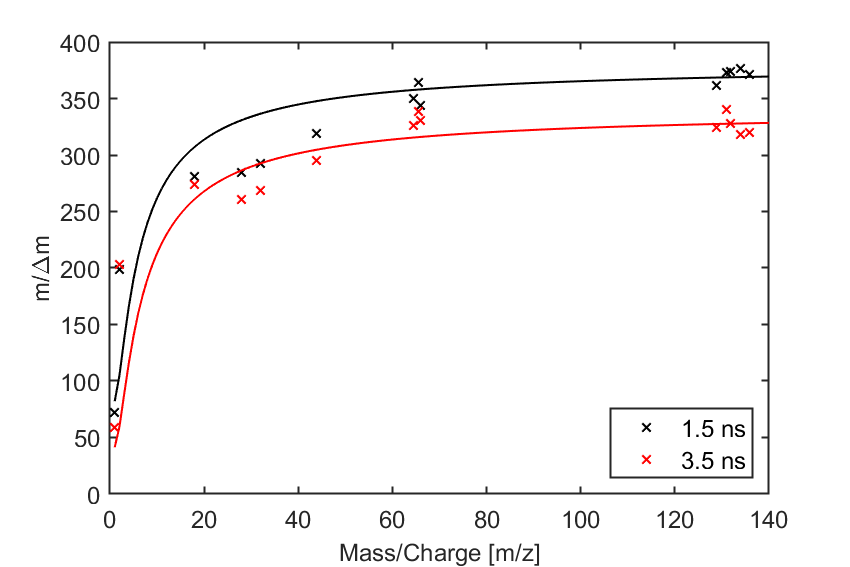
\includegraphics[width=.8\textwidth]{Bilder/PulseLabWLEm480.png}
		\caption{Measurement results of two different pulser generators with 1.5 ns and 3.5 ns fall time. Crosses are measurement points and solid lines are trend lines.}
		\label{fig:LabWLE}
	\end{figure}
	The mass resolution reaches a plateau for high mass ions because the term $dt_s$ gets dominant over the other error contributions from Eq.~\eqref{eq:dti}. $dt_s$ increases linearly with the time $t$ and therefore the mass resolution reaches a plateau for high mass ions (see Fig.~\ref{fig:Simtfall}~left). The deviation $R$ is a measure by what fraction the mass resolution of the low mass ions deviates from that plateau. The mass resolution of mass/charge ratio 200 was taken as a reference.	The calculations revealed that for low mass ions the impact of the ion temperature is negligible compared to the impact of the spatial spread $\Delta s$ and the pulse fall time $t_{fall}$. The impact of $t_{fall}$ is shown in Fig.~\ref{fig:Simtfall} left. The initial range of starting positions is $\pm$~0.4~mm which corresponds to the diameter of the electron beam in the ionisation region. With decreasing fall time, the deviation in mass resolution decreases. This is also visible in the right figure. An improvement in the fall time by one decade results in an improvement of 1~decade of the relative error. With a fall time of 1~ns, the maximum relative deviation is only 10\textsuperscript{-3}. The impact of the fall time is also visible in measurements. Fig.~\ref{fig:LabWLE} shows measurements with two different pulse generators with fall times of 1.5~ns and 3.5~ns.\\
	\begin{figure}[h!] % spatial deviation plots
		\centering
		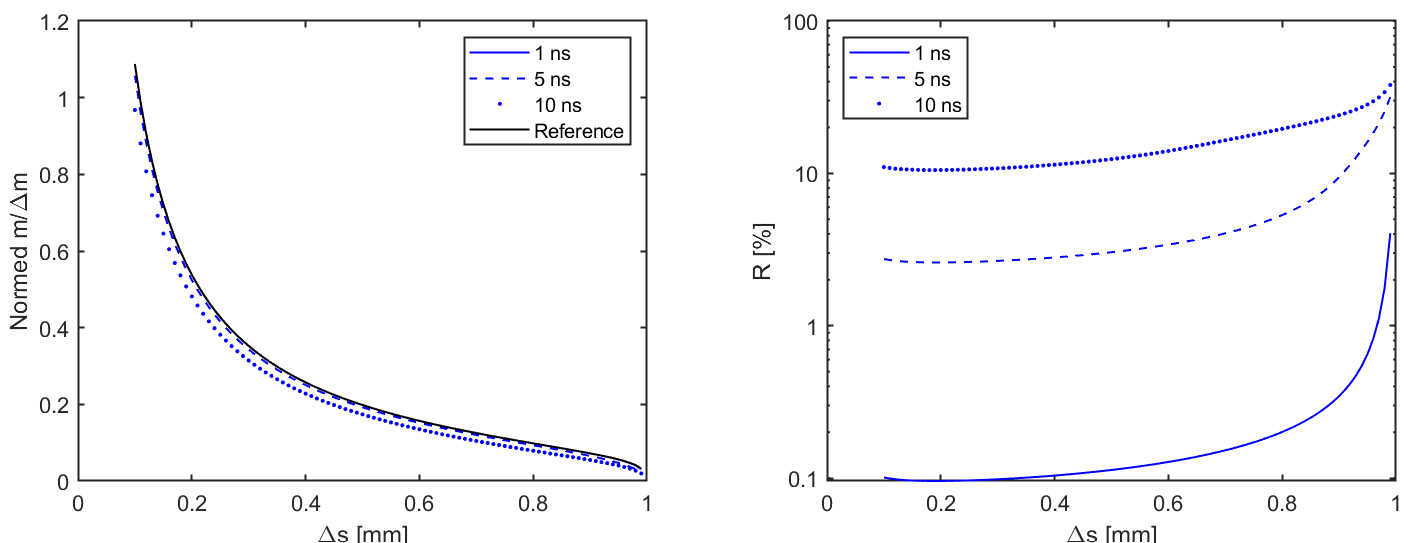
\includegraphics[width=\textwidth]{Bilder/PulseSimPosition.png}
		\caption{Left: Calculated mass resolution as a function of the spatial spread $\Delta s$ for three different pulser fall times. Right: relative deviation of the mass resolution from the plateau as a function of the mass/charge ratio.}
		\label{fig:SimtfallPos}
	\end{figure}
	Fig.~\ref{fig:SimtfallPos}~left shows the mass resolution as a function of the position deviation $\Delta s$ for mass 1~u. The ionisation region has a diameter of 2~mm. Therefore the maximal deviation of the ions is 1~mm. With increasing $\Delta s$ the mass resolution drops very rapidly. Therefore it is very important to focus the ions in the centre of the ionisation region. The better the ions are focused, the better is the mass resolution. The relative deviation increases significantly for position deviations close to 1~mm because there, some ions already leave the source when the high voltage pulse is not fully applied.\\

%----------------------------------------------------------------------------------
	\subsection{Signal-to-Noise Ratio}
	The Signal-to-Noise Ratio (SNR) is defined as the ratio of the background corrected mass peak amplitude $I_{p}$ and the standard deviation of the base line $\sigma_{Base}$ \cite{Agilent_TechNote_SNR,Master_Meyer}: % Technical Note Agilent and Masterarbeit Stefan.
	\begin{equation}
		SNR = \frac{I_{p}}{\sigma_{Base}}
		\label{eq:SNR}
	\end{equation}
	The number of detected ions is proportional to the area under the detected mass peak. Therefore, a better focusing of the ions in the time domain leads to a higher and narrower signal peak resulting in a better mass resolution and signal-to-noise ratio. This is a special feature of time-of-flight mass spectrometers: higher mass resolution results in a higher SNR. For magnetic sector instruments, the mass resolution is improved by limiting the phase space leading to a loss in signal intensity and therefore a worse signal-to-noise ratio. The noise in the spectrum originates from different sources such as from the electronics operating the instrument. Noise with a fixed frequency can be subtracted later from the signal eg. by Fourier filtering. The random noise induced by high energetic particles from Jupiter's harsh radiation field is attenuated by shielding the detector with a tungsten copper shield \cite{Foehn2021}. In addition, NIM has a special designed ion-storage source to store the produced ions during the time when no extraction pulse is applied at the ion extraction grid (Chap.~\ref{sec:setup}). Ions which are produced and not stored in the ionisation region are lost and also contribute to the random noise of the measured signal \cite{Diss_Abplanalp}. 

%-------------------------------------------------------------------------------------------
	\subsection{Filament}
		NIM uses specially designed Y\textsubscript{2}O\textsubscript{3} filaments provided by \textit{Kimball Physics, Wilton, USA} to ionise neutral particles entering the ionisation region. These filaments have an improved coating Y\textsubscript{2}O\textsubscript{3} to enhance the filament lifetime to 10'000~h of operation time. In addition, they have longer filament wires to reduce the power loss to the filament base by thermal conductivity (Fig.~\ref{fig:Y2O3Fil}). The longer wires make the filament more delicate in terms of mechanical stress. Therefore, a vibration and shock test were done, which showed no anomalies in terms of performance between the normal Y\textsubscript{2}O\textsubscript{3} and the specially designed Y\textsubscript{2}O\textsubscript{3}e filaments \cite{Diss_Fausch}. In the following sections a power estimation of these filaments is done and also a characterisation of the NIM PFM and FS filament controller boards, which provide the power for the filaments in the NIM PFM and FS instruments.
		\begin{figure}[h]
			\centering
			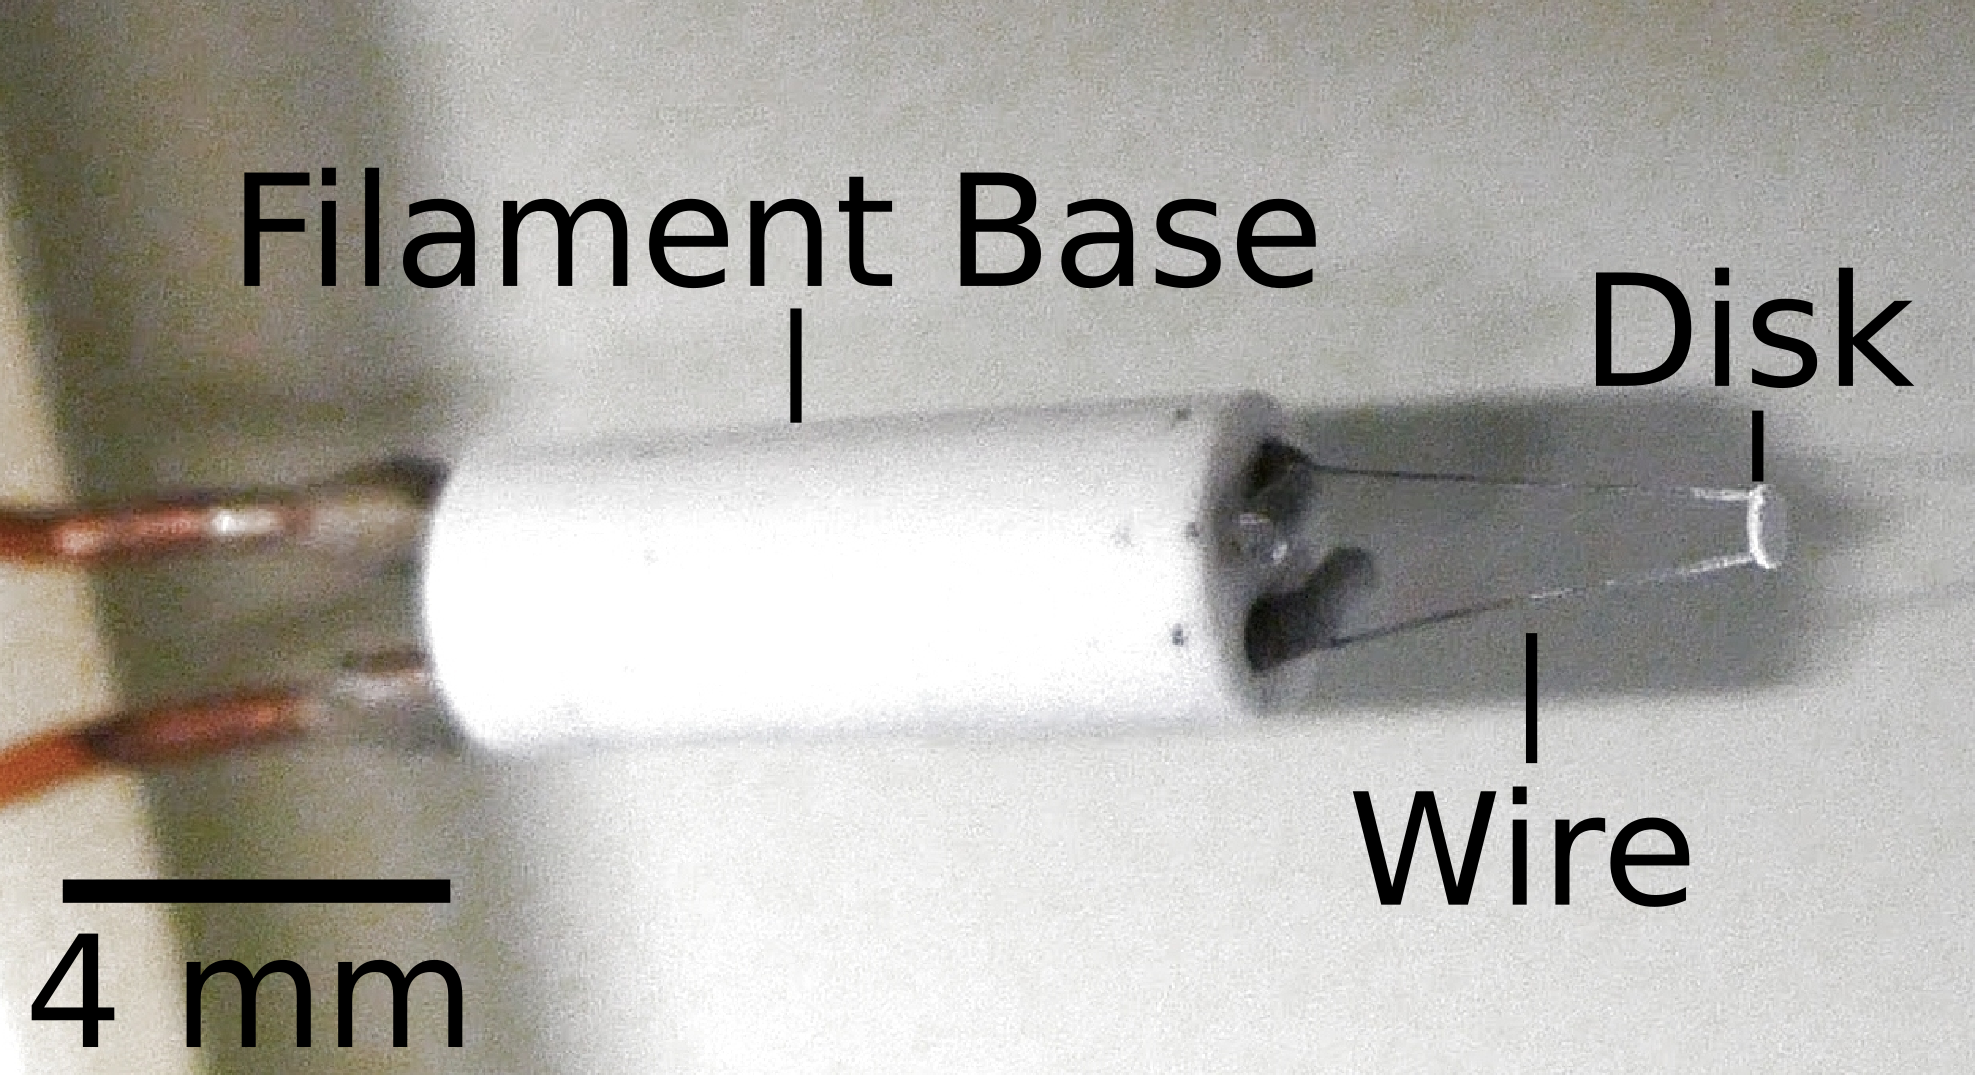
\includegraphics[width=.5\textwidth]{Bilder/Y2O3_filament.png}
			\caption{Y\textsubscript{2}O\textsubscript{3}e filament.}
			\label{fig:Y2O3Fil}
		\end{figure}

		\subsubsection{Power Calculation}
		In this chapter, the power of the Y\textsubscript{2}O\textsubscript{3}e filaments (Fig.~\ref{fig:Y2O3Fil}) used in the NIM instrument is estimated and compared with the power consumption of the standard filaments Y\textsubscript{2}O\textsubscript{3} filaments.
		% The filament wires consists of a tungsten rhenium alloy (W3Re) with a tantalum (Ta) disc coated with Yttrium oxide (Y\textsubscript{2}O\textsubscript{3}) as electron emitting material (Fig.~\ref{fig:Y2O3Fil}).
		The Y\textsubscript{2}O\textsubscript{3} is heated up by the heater current $I_{heat}$ until it emits electrons. The required temperature depends on the desired emission current $I_{em}$. The Richardson law for thermionic electron emission gives the emission current density $j$ for a material as a function of the temperature $T_D$:
		\begin{equation}
			j = A_GT_D^2e^{-\frac{W}{k_BT_D}}
			\label{eq:Richardson}
		\end{equation} % May further explain the Richardson constant. During proofreading.
		With $A_G$ the Richardson constant, which for Y\textsubscript{2}O\textsubscript{3} is 10\textsuperscript{4}~\si{\ampere\per\square\meter\per\square\kelvin} \cite{MaterHandbookCardaelli}, $W$ is the work function of Y\textsubscript{2}O\textsubscript{3} which is 2.4~eV \cite{MaterHandbookCardaelli} and $k_B$ the Boltzmann constant. The emission current $I_{em}$ is the current density multiplied by the area $A_{D}$ of the filament disk:
		\begin{equation}
			I_{em} = j\cdot A_{D}
		\end{equation}
		The total power required to reach the temperature at the disk to emit electrons is the power lost through thermal conductivity $P_{cond}$ through the thin wires connecting the filament disk with the filament base and the power lost through thermal emissivity $P_{rad}$ of the wire and the disk. This power corresponds to the power dissipated by the resistive losses $P_{R}$ of the wire:
		\begin{equation}
			P_{R} = P_{cond} + P_{rad}
		\end{equation}
		The power lost through thermal conductivity to the filament base is estimated:
		\begin{align}
			P_{cond} =& 2\cdot A_{w}k\frac{\Delta T}{l_{w}} \\
					 =& 2\cdot A_{w}k\frac{T_D - T_B}{l_{w}}
		\end{align}
		With $A_{w}$ the wire cross section, $k$ the thermal conductivity (150~W/(K~m) for W3Re \cite{thermcondTungst} and 150~W/(K~m) for Ir \cite{Ho_1972}). $\Delta T$ is the temperature difference between the disk $T_D$ and the filament base $T_B$ and $l_{w}$ the wire length. The factor 2 is because there are two legs connecting the disk with the base. % Only further explanation of the choose of k if someone asks (Average between the base and filament disk was taken.)
		The power lost through thermal radiation $P_{rad}$ is the sum of the power lost by the wire $P_{wire}$ and by the disk $P_{disk}$:
		\begin{align}
			P_{rad} =& P_{wire} + P_{disk}\\
					=& 2\sigma\cdot\epsilon_{w}\cdot A_w T_w^4 + \sigma\cdot\epsilon_{df}\cdot A_D T_D^4 + \sigma\cdot\epsilon_{db}\cdot A_D T_D^4
		\end{align}
		With $\sigma$ the Stefan-Boltzmann constant, $\epsilon_{w}$ the emissivity of the wire material (0.2 for W3Re \cite{thermcondTungst} and 0.3 for Ir \cite{Burgess1914}), $\epsilon_{df}$ the emissivity of the coating (0.5 for Y\textsubscript{2}O\textsubscript{3} \cite{ThermEmiss_Y2O3}), $\epsilon_{db}$ the emissivity of the disk material (0.325 for Ta \cite{ThermalEmiss_Ta} and 0.3 for Ir \cite{Burgess1914}) and $T_w$ the temperature of the wire. The thermal emission depends strongly on the temperature. To estimate the radiated power of the wire, the temperature profile was assumed to be linear resulting in:
		\begin{align}
			P_{wire} =& 2\sigma\epsilon_{w}2r\pi\int_{0}^{l_w} \left(\frac{\Delta T}{l_w}l + T_{B}\right)^4\cdot dl\\
					=& 2\sigma\epsilon_{w}2r\pi\int_{0}^{l_w} \left(\frac{(T_D-T_B)}{l_w}l + T_{B}\right)^4\cdot dl\\
					=& 2\sigma\epsilon_{w}2r\pi\int_{0}^{l_w} \left(  \frac{(T_D-T_B)^4}{l_w^4}l^4 + 4\frac{(T_D-T_B)^3}{l_w^3}l^3T_B \ldots \right. \nonumber \\
					& \left. \qquad\qquad\qquad + 6\frac{(T_D-T_B)^2}{l_w^2}l^2T_B^2 + 4\frac{(T_D-T_B)}{l_w}lT_B^3 + T_B^4  \right) \cdot dl
		\end{align}
		Solving the integral results in:
		\begin{align}
			P_{wire} =& 2\sigma\epsilon_{w}2r\pi\cdot l_w \left( \frac{1}{5}(T_D-T_B)^4 + (T_D-T_B)^3T_B + 2(T_D-T_B)^2T_B^2 \ldots\right.\nonumber\\
					 & \left. \qquad\qquad\qquad + 2(T_D-T_B)T_B^3 + T_B^4 \right)\\
					=& 2\sigma\epsilon_{w}2r\pi\cdot \frac{1}{5}l_w \left(T_D^4 + T_D^3 T_B + T_D^2 T_B^2 + T_D T_B^3 + T_B^4 \right)
		\end{align}
		With $r$ the wire radius and $T_{B}$ the temperature of the filament base. The power generated by ohmic losses $P_R$ is:
		\begin{align}
			P_R = RI_{heat}^2&\\
				= \rho\frac{l_w}{A_w}\cdot I_{heat}^2&
		\end{align}
		With $\rho$ the electric resistivity of the wire (0.45~\si{\micro\ohm\meter} for W3Re \cite{thermResistTungst} and 0.45~\si{\micro\ohm\meter} for Ir \cite{Arblaster2016}). The resulting total power matches the values measured in the laboratory within about 10~\%, which is good enough for this rough estimation. The Y\textsubscript{2}O\textsubscript{3}e filaments consume about 40~\% less power than the standard Y\textsubscript{2}O\textsubscript{3} filaments. The biggest loss of power is through thermal conductivity to the base, which could be reduced by 45~\%. The radiative losses of the wire increased because the wires are longer and therefore the surface area of the wire increased, leading to a bigger area to radiate.
		
		% The biggest loss in power is through thermal conductivity to the base, which makes about 70--80~\% of the whole power loss for the two filament types.
		
		% Pcond		New = 0.62 W;	68 %	Old = 1.12 W; 82 %
		% PWire		New = 0.13 W;	14 %	Old = 0.09 W;  7 %
		% PDisc		New = 0.16 W;	18 %	Old = 0.16 W; 12 %
		% Pcondrad	New = 0.91 W;			Old = 1.36 W;
		% PR		New = 0.97 W;			Old = 1.54 W;
		% Ptot		New = 0.91 W;			Old = 1.37 W;
		% PLab		New = 1 W; 				Old = 1.66 W;
		
		
		\subsubsection{Flight Filament Controller Boards Characterisation}
		In this chapter the electrical characteristics of the NIM PFM and FS controller boards used to power the electron emitting filaments in the NIM instrument are discussed.\\
		Fig.~\ref{fig:FilSampGraph} shows the electrical characteristics of the load line of a sample filament controller board (black) and a theoretical filament (blue). Note that the resistance of the tungsten heater wire increases substantially with temperature, which explains the curvature of the blue line \cite{Wilthan_2005}. The intersection of the load line with the x-axis corresponds to the maximal current the filament controller board can provide and the intersection with the y-axis corresponds to the maximal voltage. Every point below the load line can be reached by the controller board. The red curves show the lines of constant power. Depending on the desired emission current, the filament disk has to be heated to a certain temperature (Eq.~\eqref{eq:Richardson}). The higher the temperature is, the higher is the power consumption of the filament due to power losses through thermal conductivity and thermal radiation.	Therefore, a higher emission current requires higher power. The current and voltage settings for a given emission current are the intersection of the filament line with the corresponding power line.
		\begin{figure}[h!]
			\centering
			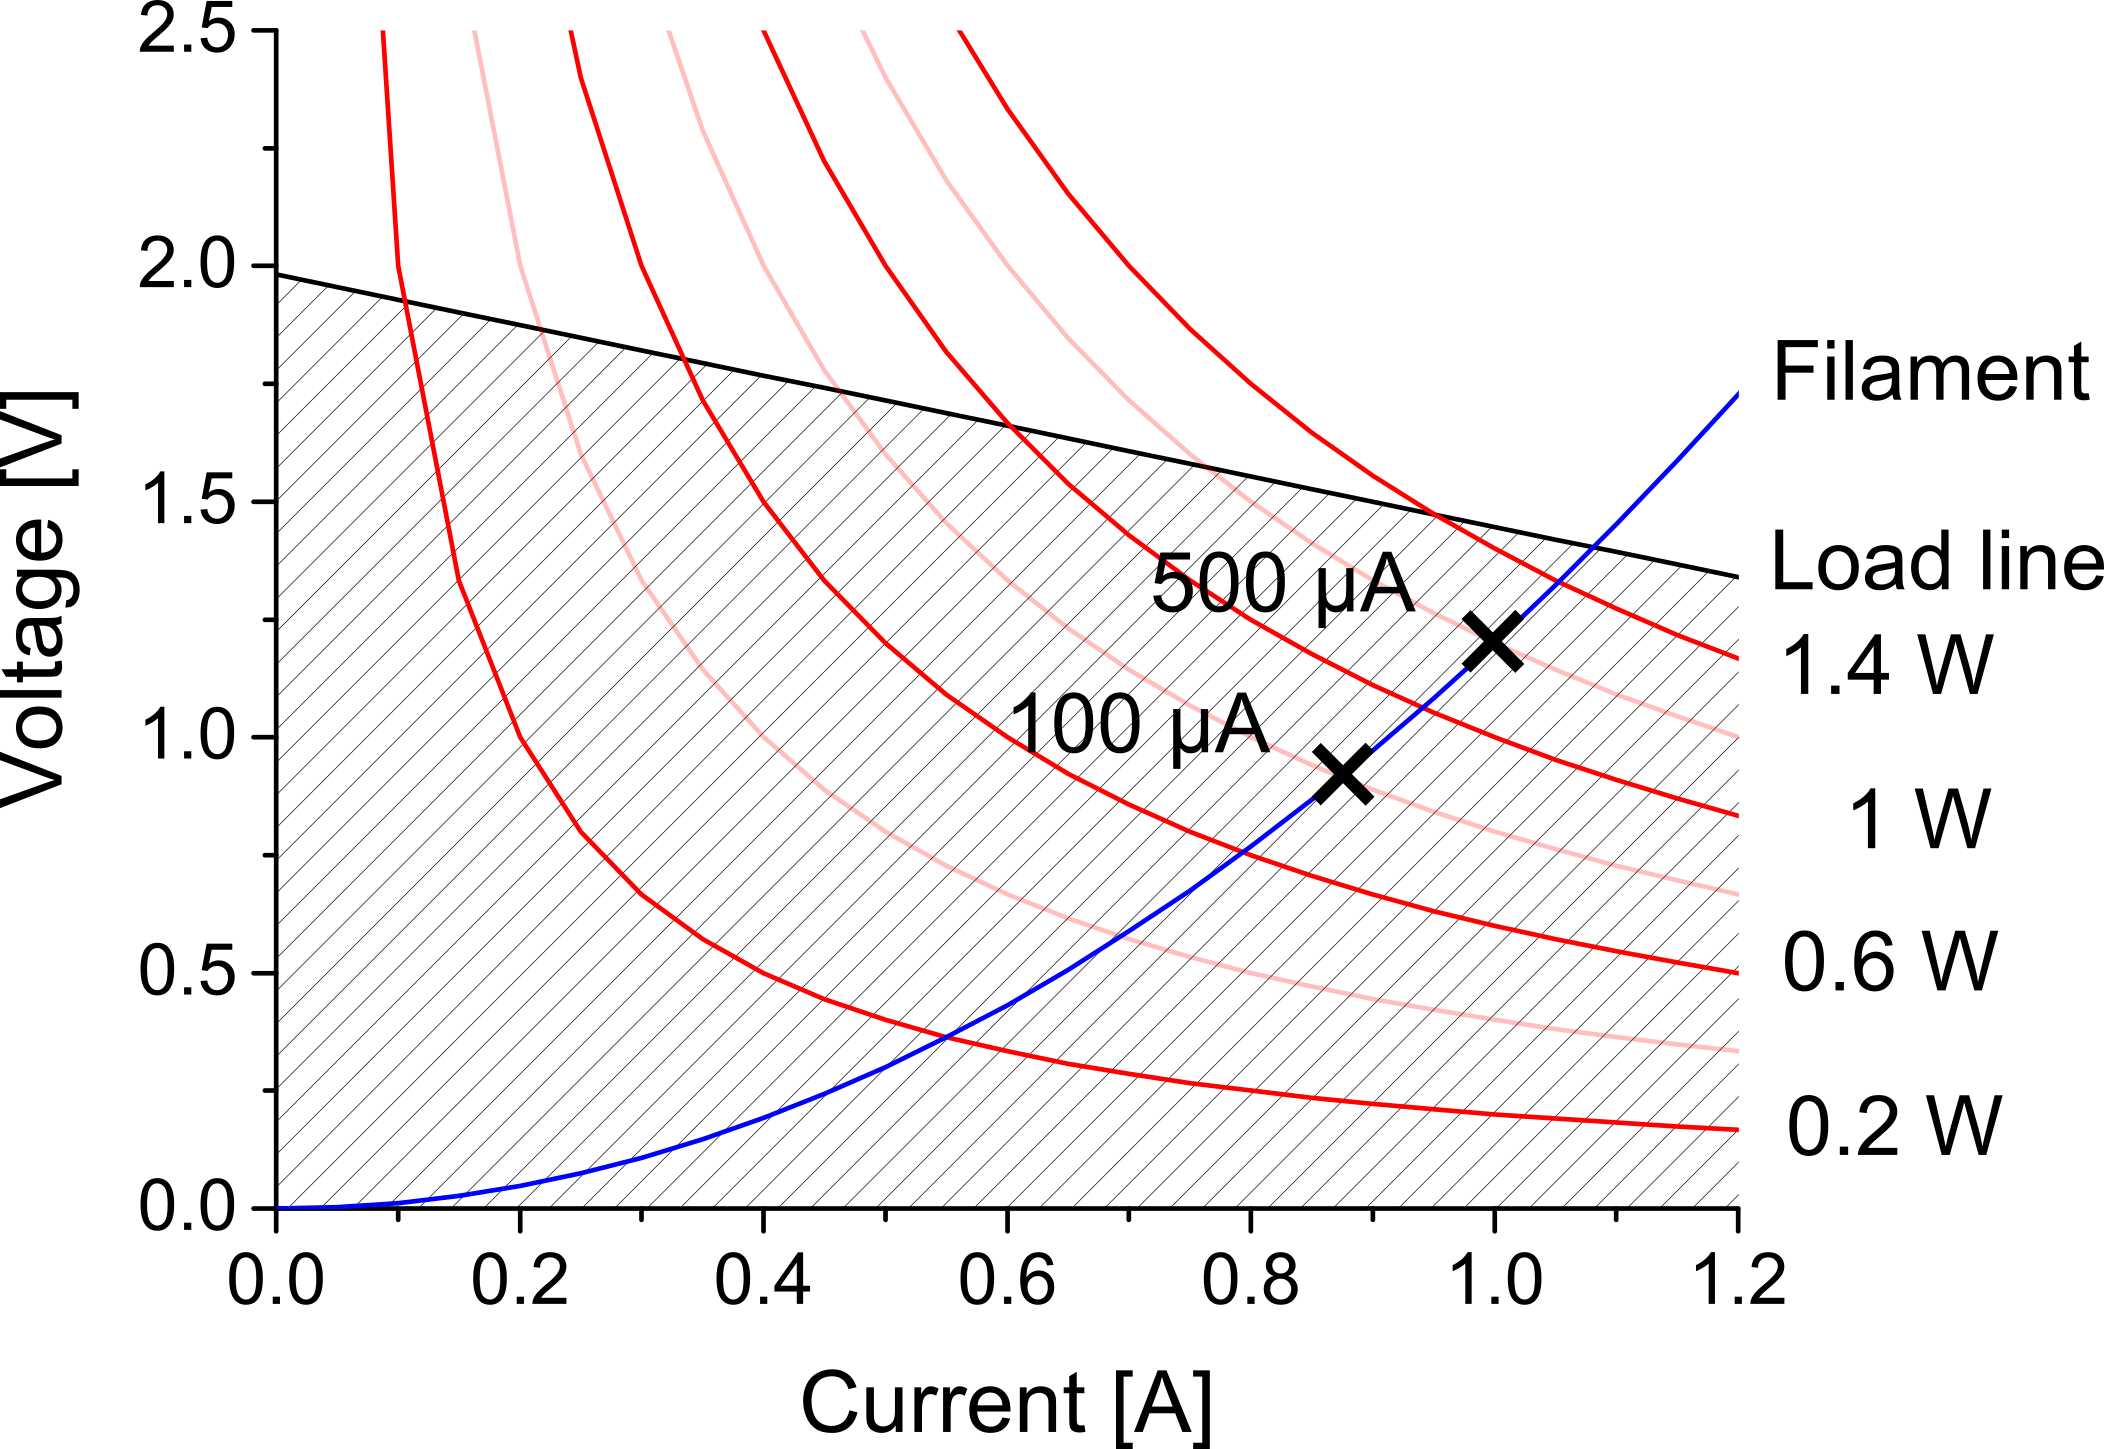
\includegraphics[width=.7\textwidth]{Bilder/Fil_SampGraph.png}
			\caption{Electrical characteristics of a sample filament (blue) and the load line of an electronic board (black). The red lines show different power levels.}
			\label{fig:FilSampGraph}
		\end{figure}
		\begin{figure}[h!]
			\centering
			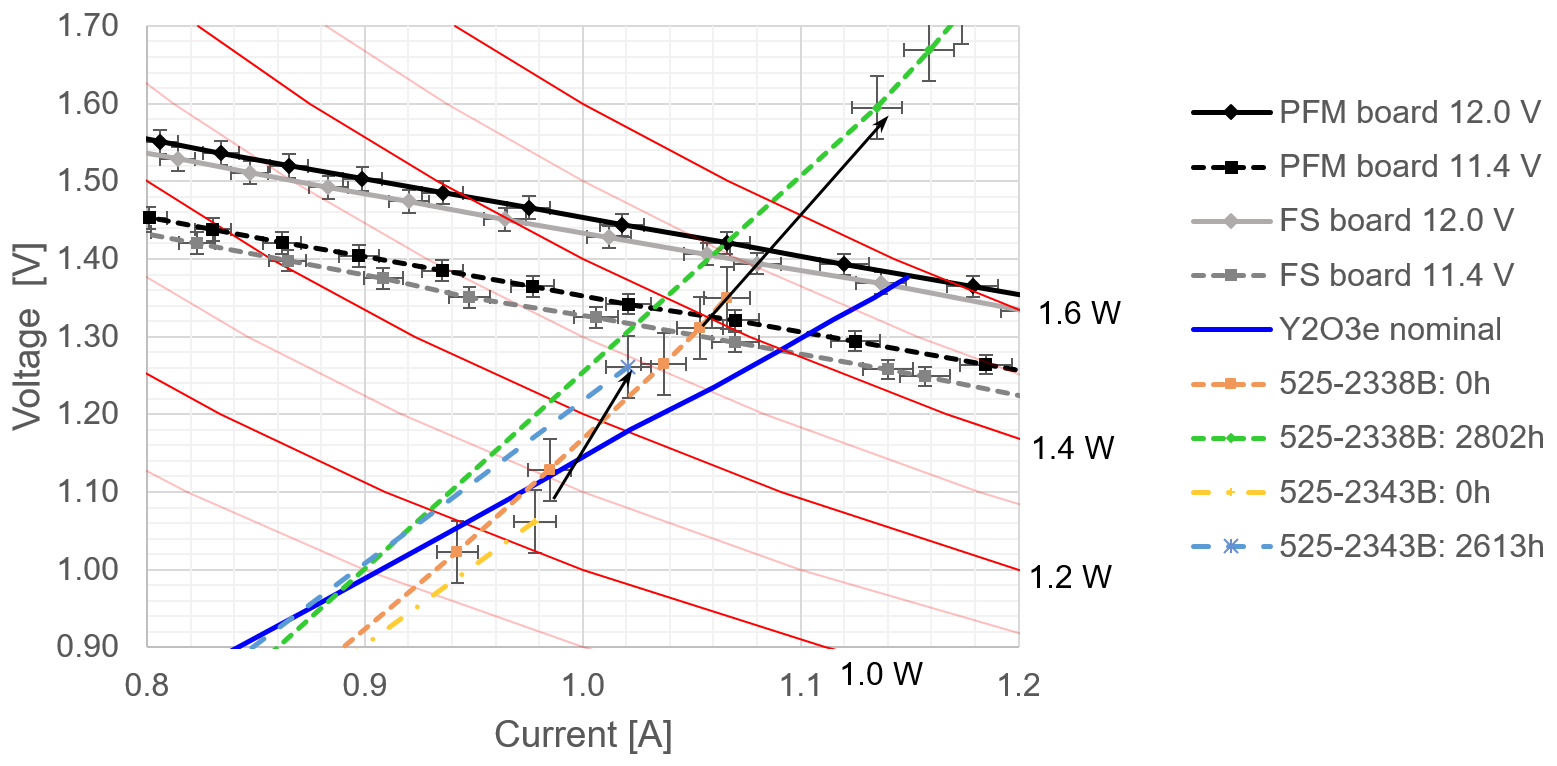
\includegraphics[width=\textwidth]{Bilder/Filament_RicosGraph.png}
			\caption{Electrical characteristics of selected Y\textsubscript{2}O\textsubscript{3}e filaments and the NIM PFM and FS controller boards showing the maximal I-V capabilities of the two power supplies at nominal supply voltage of 12.0~V and reduced supply voltage of 11.4~V. The red hyperbolas in the background show the power levels (adapted from \cite{Diss_Fausch}).}
			\label{fig:FilRico}
		\end{figure}
		For two emission currents, these points are marked as black crosses as an example.\\
		Fig.~\ref{fig:FilRico} shows the electrical characteristics of the NIM PFM (black) and FS (grey) controller boards once for nominal supply voltage of 12.0~V and once for the minimal supply voltage of 11.4~V from the DC power supply of the PEP experiment. The blue line shows the nominal behaviour of a Y\textsubscript{2}O\textsubscript{3}e filament. At the current state, long term tests with filaments at different emission currents are running to verify their operation time of 10'000~h. The filaments displayed in this graphic are the one with the worst electrical characteristics from each batch. Filament 525-2343B has a target emission current of 50~\si{\micro\ampere} and filament 525-2338B has a target emission current of 300~\si{\micro\ampere}. For a bad filament such as 525-2338B the flight controller boards could not provide the required power. If the target emission is 50~\si{\micro\ampere} the two boards can provide the power even after 2300~h of operation time. The difference in performance between the nominal filament and the filaments used in our tests originates from the different test setups in which the filaments were tested. The extraction fields in the test setup of the nominal filament were set to optimise electron emission to minimise power consumption. This is not a realistic case for a flight instrument where the extraction fields also have to focus the electron beam in the ionisation region. Therefore, the test setup for the long term tests was built as a replicate of NIM's electron extraction region. The applied extraction voltages are set to nominal values used during filament operation. Therefore, the filaments are more stressed than in a setup which is optimised to extract the electrons from the filament disk \cite{Diss_Fausch}.
		
		
%-------------------------------------------------------------------------------------------	
	\subsection{Ion Storage}\label{chap:TheoIonStor}
	Ion storage of positive ions in the ionisation region is mainly achieved by the negative space charge potential of the electron beam. Together with the other focusing electrodes in the ionisation region, a 3D electrostatic trapping field is generated to store the ions produced during the time when no high-voltage pulse is applied on the extraction grid (IS~5 in Fig.~\ref{fig:ISZoom}). NIM has a nominal duty cycle of 10~kHz and the pulse duration of the extraction pulse is 1--2~$\mu$s. In the remaining 98~$\mu$s per cycle ions are produced, which have to be stored in the source between two extraction pulses because lost ions add to the random noise level reducing the signal-to-noise ratio. In the following section, the potential in the centre of the electron beam is calculated. The electron emission current $I_{e}$ is:
	\begin{equation}
		I_{e} = n_e q_0 v\pi R_e^2
		\label{eq:theoElIem}
	\end{equation}
	With $n_e$ the electron number density, $q_0$ the elementary charge, $v$ the velocity of the electrons and $R_e$ the radius of the electron beam (Fig.~\ref{fig:thAntIs}). The electrons get accelerated by the negative potential applied at the filament base. This potential is --70~\si{\volt} resulting in a kinetic energy $U$ of 70~\si{\electronvolt}. The velocity of the electrons is:
	\begin{equation}
		v = \sqrt{\frac{2 U}{m_e}}
		\label{eq:theoElIemVelo}
	\end{equation}
	With $m_e$ the mass of the electron. Solving Eq.~\eqref{eq:theoElIem} for the volume density $n_e$ and inserting Eq.~\eqref{eq:theoElIemVelo} for the velocity results in:
	\begin{equation}
		n_e = \frac{I_e}{q_0 \pi R_e^2}\sqrt{\frac{m_e}{2U}}
		\label{eq:theoElIemNe}
	\end{equation}
	The electric field $E(r)$ from the space charge of the electron beam in the ionisation region is calculated for $R_e<r<h_{Is}/2$ with $r$ the distance from the centre of the beam and $h_{Is}$ the height of the ion source. The electric flux is defined as the surface integral of the electric field through the surface of an enclosed volume, which is in this case a cylinder volume. Using Gauss's law the electric flux through the beam surface $A_{beam}$ is equal to the total charge $Q$ inside the cylinder volume. In this calculation, the base and deck area are neglected:
	\begin{align}
		A_{beam} E(r) &= \frac{Q}{\epsilon_0}\\
		2\pi r l E(r) &= \pi R_e^2 l n_e q_0 \frac{1}{\epsilon_0}
	\end{align}
	With $l$ the cylinder length, $q_0$ the elementary charge and $\epsilon_0$ the vacuum permittivity. Replacing the number density $n_e$ with Eq.~\eqref{eq:theoElIemNe} and solving the equation for the electric field $E(r)$ results in:
	\begin{equation}
		E(r) = \frac{I_e}{2 \pi \epsilon_0} \sqrt{\frac{m_e}{2U}}\frac{1}{r}
	\end{equation}
	The potential $\Phi_o (r)$ at a position $r$ outside of the electron beam is:
	\begin{equation}
		\Phi_o (r) = -\int_{h_{Is}/2}^{r} E(r') dr' = -\frac{I_e}{2\pi\epsilon_0}\sqrt{\frac{m_e}{2U}}\ln\left(\frac{r}{h_{Is}/2}\right)
	\end{equation}
	The electric field inside the electron beam at position $0<r<R_e$ is calculated by using again Gauss's law:
	\begin{equation}
		2\pi r l E(r) = \pi r^2 l n_e q_0 \frac{1}{\epsilon_0}
	\end{equation}
	Replacing the number density $n_e$ with Eq.~\eqref{eq:theoElIemNe} and solving the equation for the electric field $E(r)$ results in:
	\begin{equation}
		E(r) = \frac{I_e}{2\pi\epsilon_0}\sqrt{\frac{m_e}{2U}}\frac{r}{R_e^2}
	\end{equation}
	The electric potential $\Phi_i (r)$ is:
	\begin{equation}
		\Phi_i (r) = -\int_{R_e}^{r} E(r') dr' = -\frac{I_e}{4\pi\epsilon_0}\sqrt{\frac{m_e}{2U}}\left(\frac{r^2}{R_e^2} -1 \right)
	\end{equation}
	And relative to the border of the ion source:
	\begin{equation}
		\Phi_i (r) = -\frac{I_e}{4\pi\epsilon_0}\sqrt{\frac{m_e}{2U}}\left(2\ln\left(\frac{R_e}{h_{Is}/2}\right) +\frac{r^2}{R_e^2} -1 \right)
		\label{eq:elPotIem}
	\end{equation}
	For an electron emission current of 100~\si{\micro\ampere} the electric potential in the centre of the electron beam is 0.75~\si{\volt}. This potential well is deep enough to trap ion species at thermal energies. For faster species, NIM has a special designed ionisation region (Fig.~\ref{fig:ISZoom}). The electrodes IS~1, IS~5 and IS~6 trap the ions in x-direction where the two ring electrodes IS~2 and IS~4 trap the ions in the other two directions.		
	\begin{figure}[h]
		\centering
		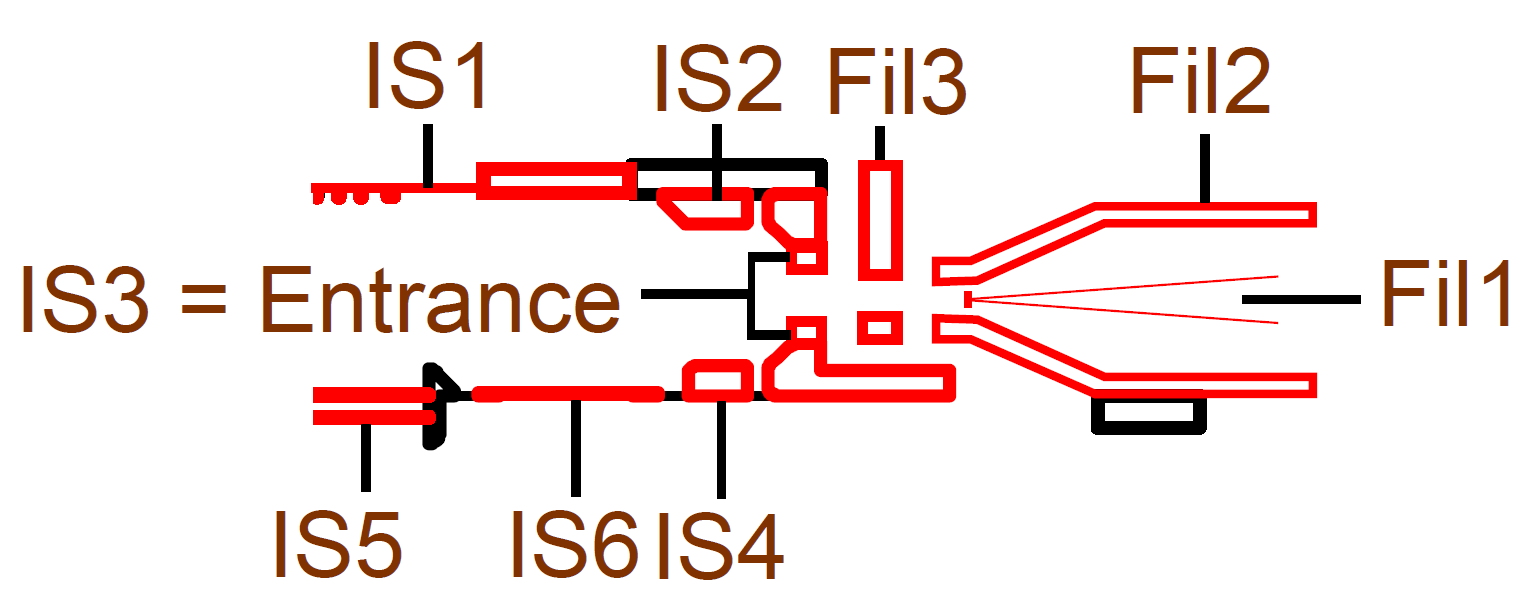
\includegraphics[width= .5\textwidth]{Bilder/NIM_schema_zoom_IS.png}
		\caption{Detail of NIM's ionisation region.}
		\label{fig:ISZoom}
	\end{figure}
	\begin{figure}[h]
		\centering
		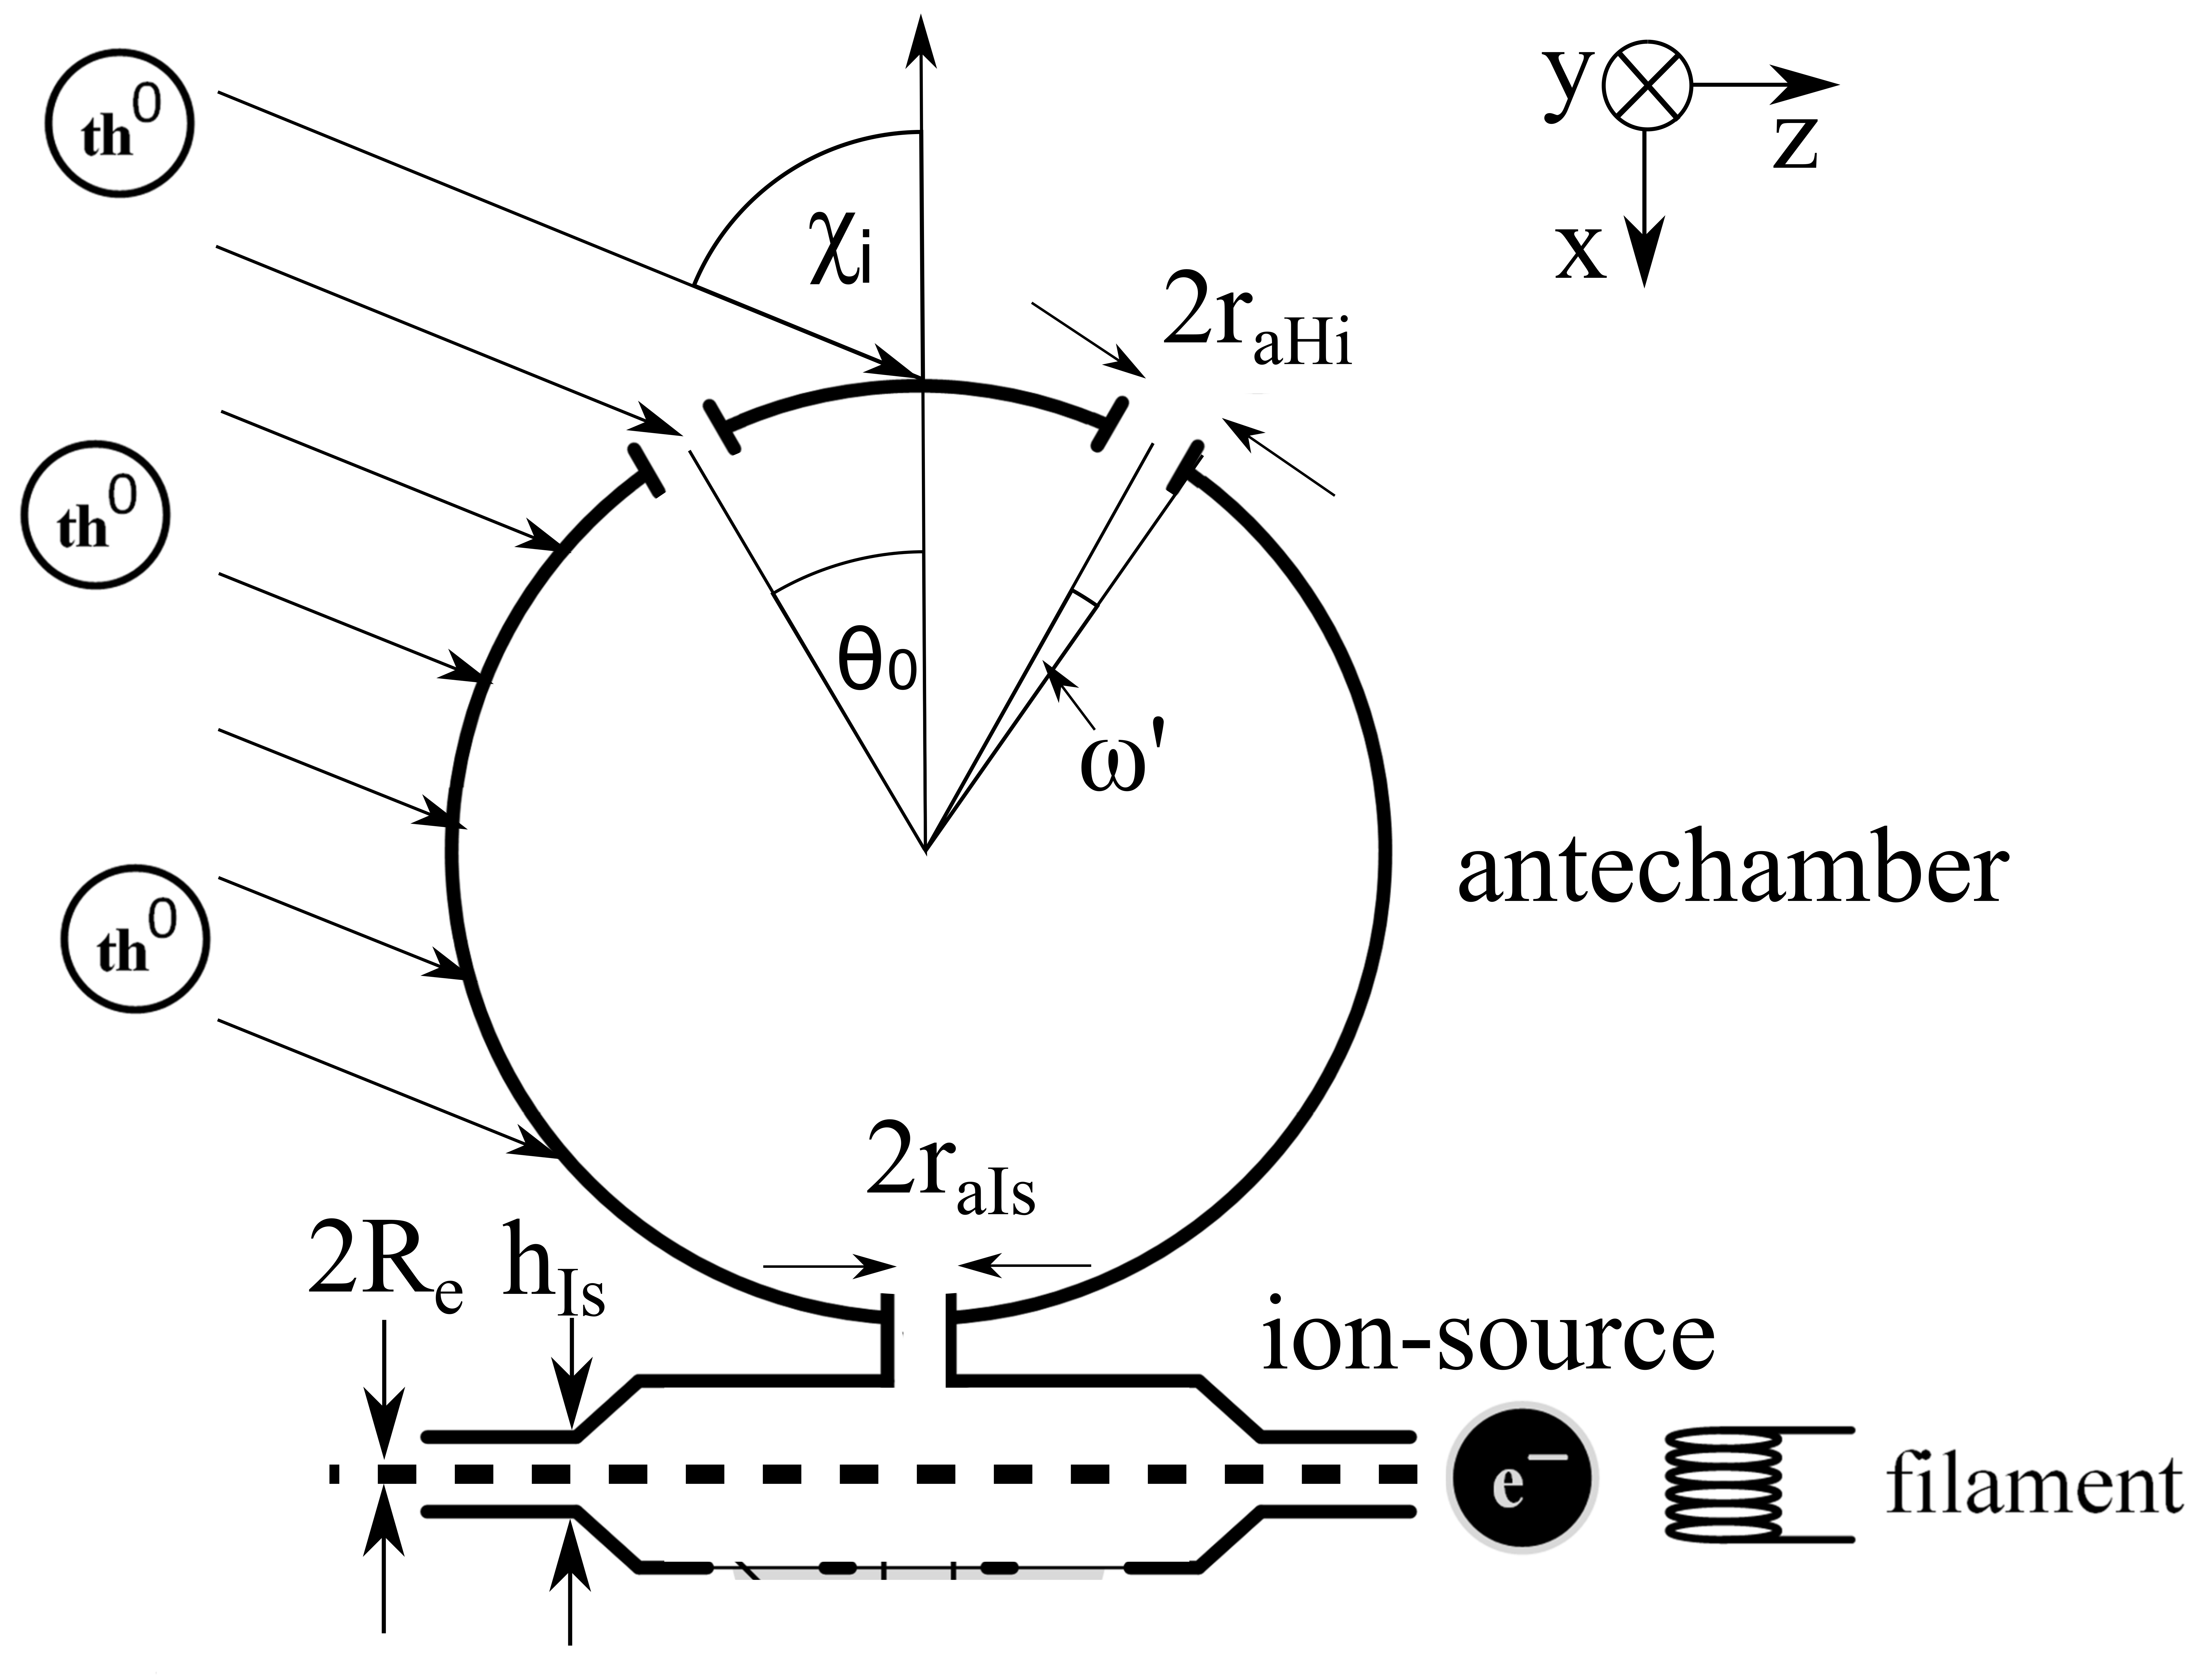
\includegraphics[width= 0.7\textwidth]{Bilder/particleDensEnh.png}
		\caption{Schematics of the antechamber and the ionisation region.}
		\label{fig:thAntIs}
	\end{figure}

%----------------------------------------------------------------------------------------------------
	\subsection{Density enhancement of a Closed Source}\label{subsubsec:Densenhan}
	
	NIM has an open source entrance where neutral particles and ions enter the ionisation region directly and a closed source entrance where particles enter the ionisation region after being thermalised in an antechamber. In this chapter the density enhancement of the closed source entrance is determined. The density enhancement model described in \cite{DensEnhan_Wurz_07} is used and adapted for the geometry of NIM's antechamber. The particle density $n_{cs}$ in the ionisation region is:
	\begin{equation}
		\frac{n_{cs}}{n_a} = \sqrt{\frac{T_a}{T_s}}\cdot\frac{k\cdot \sin^2\big(\frac{\omega}{2}\big)\cdot \cos^2\big(\frac{\omega}{2}\big)}{1-k\cdot \cos^2\big(\frac{\omega}{2}\big)}\frac{\big(F(S_1)+ F(S_2)\big)}{2} \frac{r_{aIs}^2\cdot a}{2\cdot r_{aHi}^2 + r_{aIs}^2\cdot a}
		\label{eq:thDensEnhan}
	\end{equation}
	With:
	\begin{equation}
		F(S_i)) = e^{-S_i^2} + \pi^{1/2}\cdot S_i\cdot\big(1 + {\rm erf}(S_i)\big)
		\label{eq:F(S)}
	\end{equation}
	% cos(chi) = cos(theta_0)cos(theta) +- sin(theta_0)sind(theta)cos(phi)
	With $n_a$ the ambient particle density of the gas outside the instrument. For the tests in the laboratory $n_a$ is the particle density of the neutral gas beam. In flight, the ambient particle density is the particle density of the moons atmosphere. $T_a$ is the temperature of the ambient gas. In the laboratory it is the temperature of the neutral particle beam. $T_s$ is the temperature of the antechamber. $k$ is the probability of a particle being re-emitted after colliding with the antechambers inner surface during thermalisation and is close to 1 because otherwise the particle would be absorbed. $\Omega$ is the total solid angle of all openings leading into the antechamber. NIM has two entrance holes with the same hole diameter and therefore the total solid angle $\Omega$ is the sum of the two solid angles of the entrance holes $\Omega'$:
	\begin{equation}
		\Omega = 2\cdot\Omega'
	\end{equation}
	All openings into the antechamber have a circular shape therefore, the solid angle $\Omega$ is replaced by an angle $\omega$ in the x-z-plane to simplify the equation Eq.~\eqref{eq:thDensEnhan} \cite{Hedin_1964}: 
	\begin{align}
		2\pi(1- \cos(\omega)) &= 2\cdot 2\pi(1- \cos(\omega'))\\
		\cos(\omega) &= 2\cos(\omega') -1\\
		\omega &= \cos^{-1}(2\cos(\omega') -1)
	\end{align}
	$\omega'$ is the half angle of one entrance hole (Fig.~\ref{fig:thAntIs}). $S_i$ in Eq.~\eqref{eq:F(S)} is the speed ratio along the normal axis of the entrance holes:
	\begin{equation}
		S_i = 
		\begin{cases}
			0, & \cos(\chi \pm \theta_0) < 0\\
			v_{sc}\cdot \cos(\chi + \theta_0)\cdot \sqrt{\frac{m}{2k_B T_a}}, & i=1\\
			v_{sc}\cdot \cos(\chi - \theta_0)\cdot \sqrt{\frac{m}{2k_B T_a}}, & i=2
		\end{cases}
	\end{equation}
	with $v_{sc}$ the velocity of the neutral gas beam relative to the antechamber corresponding to the spacecraft velocity, $m$ the average particle mass of the gas and $k_B$ the Boltzmann constant. $\chi$ is the angle of the test gas relative to the x-axis of the instrument and $\theta_0$ is the angle between the x-axis and the axis normal of the entrance hole. $\chi \pm \theta_0$ is the angle between the normal axis of the entrance hole and the gas inflow direction. $\chi \pm \theta_0$ has to be between $\pm 90\degree$ to enter the antechamber which implies that $\cos(\chi \pm \theta_0)$ cannot have negative values. $i=1$ is the index of one of the two entrance holes and $i=2$ is the index of the other entrance hole. The antechamber has three openings for the gas to flow out of the antechamber. The last term in Eq.~\eqref{eq:thDensEnhan} gives the ratio of how many particles leave the antechamber through the hole connecting the antechamber with the ionisation region compared to the amount of particles leaving the antechamber through the two entrance holes. The radius of the entrance holes is $r_{aHi}$ and the radius of the hole connecting the antechamber with the ionisation region is $r_{aIs}$. This term takes the molecular flow conductance of the different holes into account. The molecular flow conductance of a thermalised gas is:
	\begin{equation}
		C_0 = A\bar{v}/4
		\label{eq:theoMolFlowCondC0}
	\end{equation}
	with $A$ the cross-section of the opening and $\bar{v}$ the average velocity of the thermalised gas flowing through that opening. This formula is only valid in case the length of the tube is close to zero. Otherwise, the transmission probability $a$ has to be added resulting in:
	\begin{equation}
		C = C_0 \cdot a
		\label{eq:theoMolFlowCondCEff}
	\end{equation}
	The transmission probability depends on the length-to-radius ratio $L/R$ of the opening. van Essen and Heerens \cite{molFlowTubeTransm_Essen1976} compared different models to determine the transmission probability and calculated the values for specific length-to-radius ratios. The model that comes closest to reality is the one by Nawyn and Meyer (published by \cite{molFlowTubeTransm_Essen1976}). To calculate the transmission probability for any length-to-radius ratio, the data resulting from Nawyn and Meyer's model were fitted with the following function:
	\begin{equation}
		a = y_0 + y_1\left(1-e^{-\frac{L/R}{t_1}}\right) + y_2\left(1-e^{-\frac{L/R}{t_2}}\right)
		\label{eq:MolFloConFitFunc}
	\end{equation}
	
	\begin{table}[H]
		\begin{center}
			\begin{tabular}{|l r| l r|}
				\hline
				$y_0$	& $0.998 \pm 0.001$ & $t_1$	& $7.4 \pm 0.3$	\\
				$y_1$	& $-0.48 \pm 0.01$ & $t_2$	& $1.13 \pm 0.04$ \\
				$y_2$ 	& $-0.45 \pm 0.01$	& &\\
				\hline
			\end{tabular}
		\end{center}
		\caption{Fit parameters of Eq.~\eqref{eq:MolFloConFitFunc}.}
		\label{tab:thMolFloConFiPara}
	\end{table}
	The fit parameters are listed in Table~\ref{tab:thMolFloConFiPara}. For the two gas entrance openings of the antechamber $a$ is 1 because they have a sharp edge and therefore the length of the opening is close to zero. 
	The opening between the antechamber and the entrance has a length-to-diameter ratio of 8 resulting in a $a = 0.23$. The amount of gas flowing through this opening relative to the total outflow is:
	\begin{align}
		G_{open} & = \frac{C_{aIs}}{C_{aIs} + 2\cdot C_{aHi}} \label{eq:GAntOpen}\\
		G_{open} & = \frac{\frac{r_{aIs}^2\cdot a\cdot \bar{v}}{4}}{\frac{r_{aIs}^2\cdot a\cdot \bar{v}}{4} + 2\frac{r_{aHi}^2\cdot \bar{v}}{4}}\\
		G_{open} &= \frac{r_{aIs}^2\cdot a}{r_{aIs}^2\cdot a + 2\cdot r_{aHi}^2}
		\label{eq:geoOpenTube}
	\end{align}
	With $r_{aIs} = 2~\si{\milli\meter}$ and $r_{aHi} = 2.5~\si{\milli\meter}$ resulting in $G_{open} = 0.067$ meaning that about 6.7\% of all particles entering the antechamber actually reach the ionisation region due to losses of the geometry.\\
	\begin{table}[H]
		\begin{center}
			\begin{tabular}{|l r |l r |l r|}
				\hline
				$T_a$ 	& 295 K	& $r_{aHi}$	& 2.5~mm	& $\chi$	& 0\degree \\
				$T_s$ 	& 320 K & $r_{aIs}$ & 2~mm	& $\theta_0$& 30\degree\\	
				$k$		&	1	& $v_{sc}$	& 2.5~km/s& $m$		& 18 u\\
				$a$		& 0.23	&			&			&			&	\\
				\hline
			\end{tabular}
		\end{center}
		\caption{Values used for the variation of the different variables of the amplification factor of the antechamber (Eq.~\eqref{eq:thDensEnhan}).}
		\label{tab:thDensEnhan}
	\end{table}
	\begin{figure}[h!] % T_a T_s
		\centering
		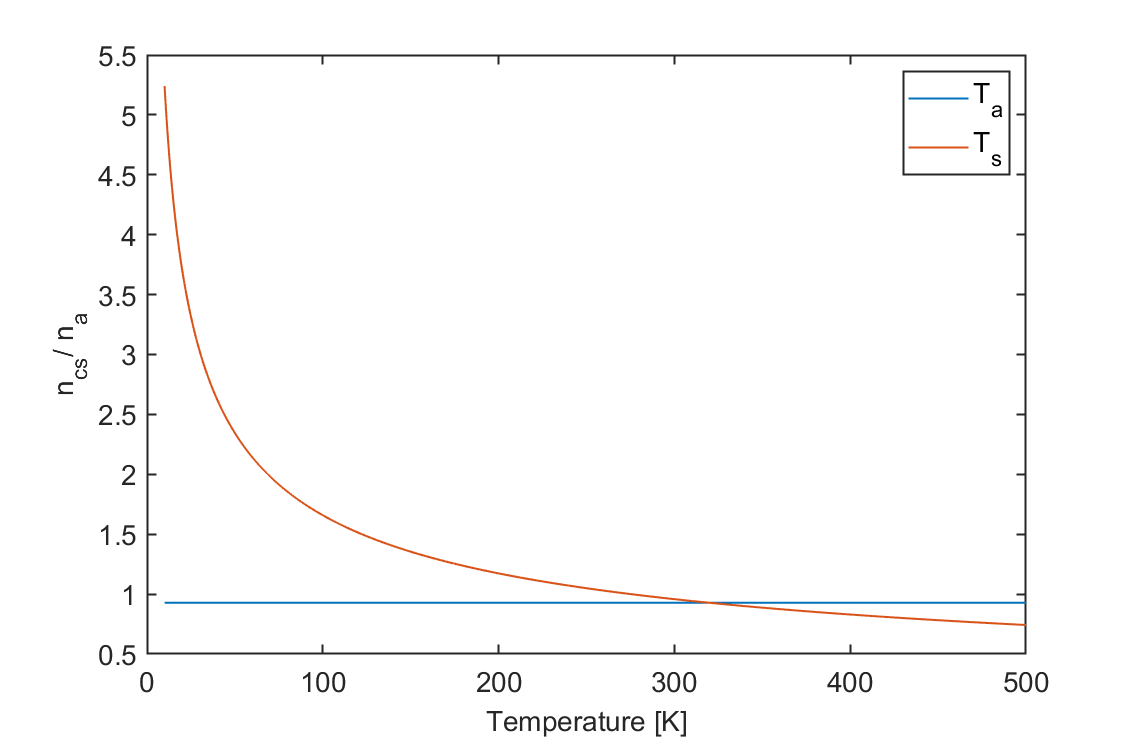
\includegraphics[width= .7\textwidth]{Bilder/Ta_Ts.png}
		\caption{Density enhancement $n_{cs}/n_a$ of the antechamber as a function of the ambient gas temperature $T_a$ and the temperature of the antechamber wall $T_s$ according to Eq.~\eqref{eq:thDensEnhan}.}
		\label{th:densEnhTaTs}
	\end{figure}
	\begin{figure}[h!] % raHi raIs
		\centering
		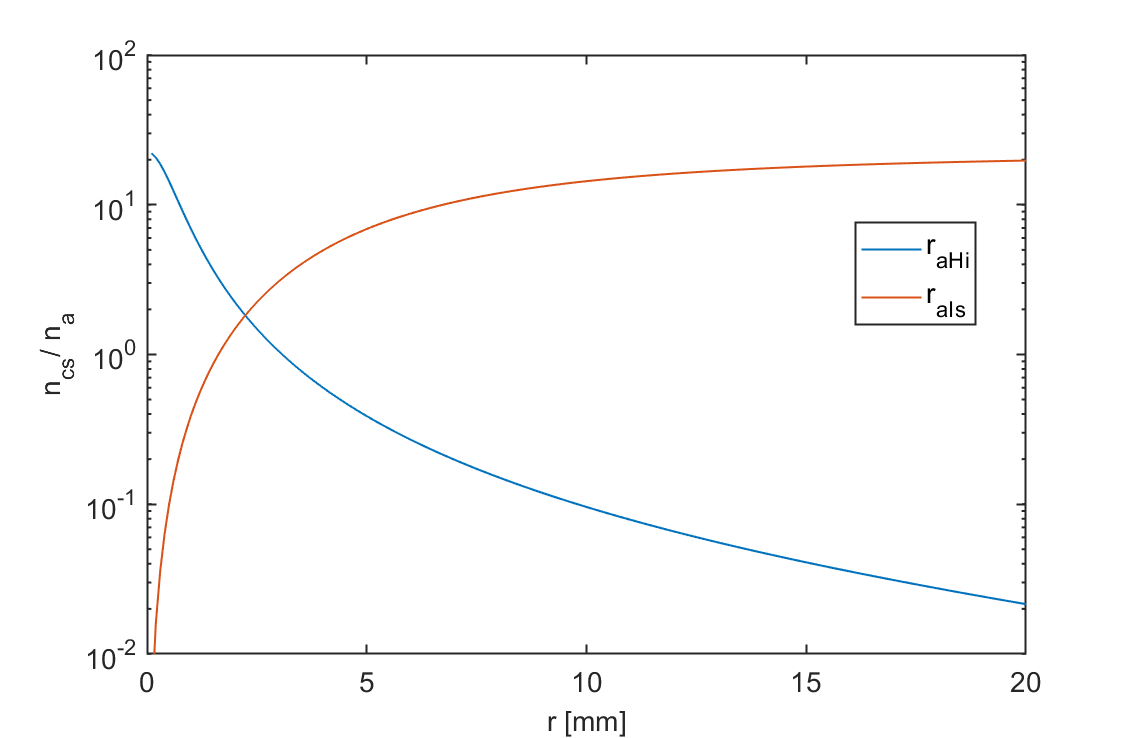
\includegraphics[width= .7\textwidth]{Bilder/raHi_raIs.png}
		\caption{Density enhancement $n_{cs}/n_a$ of the antechamber as a function of the entrance hole radius $r_{aHi}$ and the radius connecting the antechamber with the ionisation region $r_{aIs}$.}
		\label{th:densEnhraHiraIs}
	\end{figure}
	In the following section the different parameters of the density enhancement equation Eq.~\eqref{eq:thDensEnhan} were varied to determine their impact. For this analysis the particle density in the ionisation region $n_{cs}$ was divided by the particle density of the test gas $n_a$ outside of the antechamber and $n_a$ was set 1 to get the amplification of the antechamber. For this analysis the parameters were set according to Table~\ref{tab:thDensEnhan} unless otherwise mentioned. The temperatures are the ones used in the laboratory. The used particle velocity was 2.5~km/s because it is the velocity of the spacecraft in Ganymede orbit and therefore the velocity at which most of the measurements will be done. The particle reflection coefficient $k$ of the inner coating of the antechamber was set 1 assuming an ideal coating reflecting all particles. The transmission probability $a$ of the hole connecting the antechamber with the ionisation region, the radius of the antechamber entrance holes $r_{aHi}$, the radius of the hole connecting the antechamber with the ionisation region $r_{aIs}$ and the angular position of the entrance holes $\theta_0$ are defined by the geometry of the antechamber. $\chi$ was set to 0\degree. The main gas inflow direction lies then between the two entrance holes. The used test gas was water with a unit mass of 18~u.\\ % Fig. T_a T_s
	The first parameter that was varied was the gas temperature $T_a$. This temperature can be varied between 0 and 1000~K without significantly influencing the density enhancement of the antechamber (Fig.~\ref{th:densEnhTaTs}). When looking closer, a slight increase in density enhancement is observed with increasing temperature.\\
	The temperature of the antechamber $T_s$ has a bigger impact on the density enhancement. Ideally this temperature should be as low as possible to slow down the particles when they hit the chamber inner walls (see also Eq.~\eqref{eq:thDensEnhan}). When the temperature of the antechamber is too low, the gas condenses at the antechamber walls. Therefore, the particle reflection coefficient of $k$ will decrease with decreasing temperature depending on the particle species. For this calculation, this effect was ot taken into account. In flight, the antechamber is kept at temperatures higher than --17~\si{\degreeCelsius} during measurements to avoid condensation on the antechamber walls.\\
	The radius $r_{aIs}$ of the hole connecting the antechamber with the ionisation region has to be as big as possible. A bigger radius leads to a smaller length-to-diameter ratio resulting in a bigger transition probability $a$. The amount of gas flowing into the ionisation region increases (Fig.~\ref{th:densEnhraHiraIs}). The radius of the entrance holes $r_{Hi}$ should be as small as possible to increase the number of collisions of the neutral particles with the antechamber walls to thermalise them. In addition, when the entrance holes are big, a big amount of gas flows out through them. From that perspective, the biggest gain is achieved when the radius of the entrance hole is close to zero. Eq.~\eqref{eq:thDensEnhan} does not take into account that at a certain opening radius is needed to allow particles to enter the antechamber for being amplified. The equation is only valid for small openings to guaranty enough collisions of the gas with the chamber walls. Therefore, the requirement was that the area of all openings of the antechamber has to be 10\% of the total sphere surface.\\
	It is very important to take materials with a high particle reflection coefficient $k$ for the coating of the antechamber's inner surface. The particle reflection coefficient gives the probability of a particle being re-emitted when hitting the surface thus this value has to be close to 1. NIM has a gold coated antechamber because gold is electrically conductive preventing the surface from charging in the strong radiation field of Jupiter. In addition, gold is chemically inert and therefore, there is a low probability of building chemical bonds with the gas induced into the antechamber. Fig.~\ref{th:densEnhk} shows the density enhancement of the antechamber as a function of $k$. Already a change of 1\textperthousand~ has a huge impact. The impact of $k$ also depends on $\omega$.
	\begin{figure}[h!] % k
		\centering
		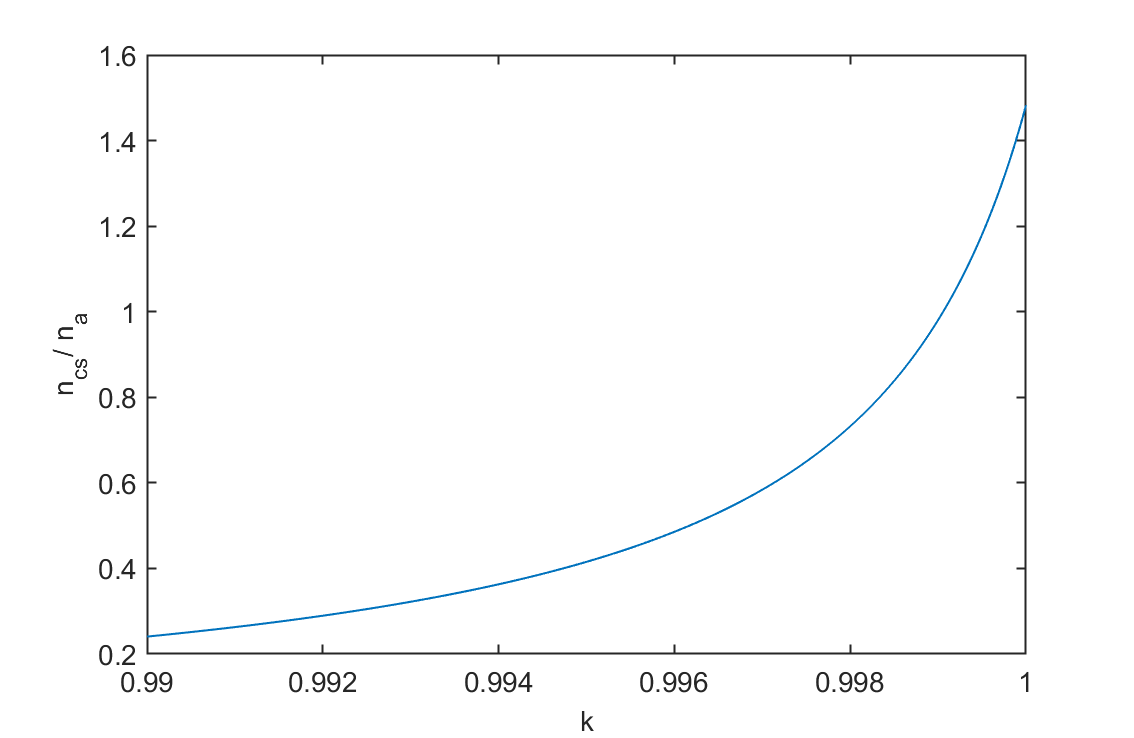
\includegraphics[width= .7\textwidth]{Bilder/k.png}
		\caption{Density enhancement $n_{cs}/n_a$ of the antechamber as a function of the particle reflection coefficient $k$.}
		\label{th:densEnhk}
	\end{figure}
	\begin{figure}[h!] % mass
		\centering
		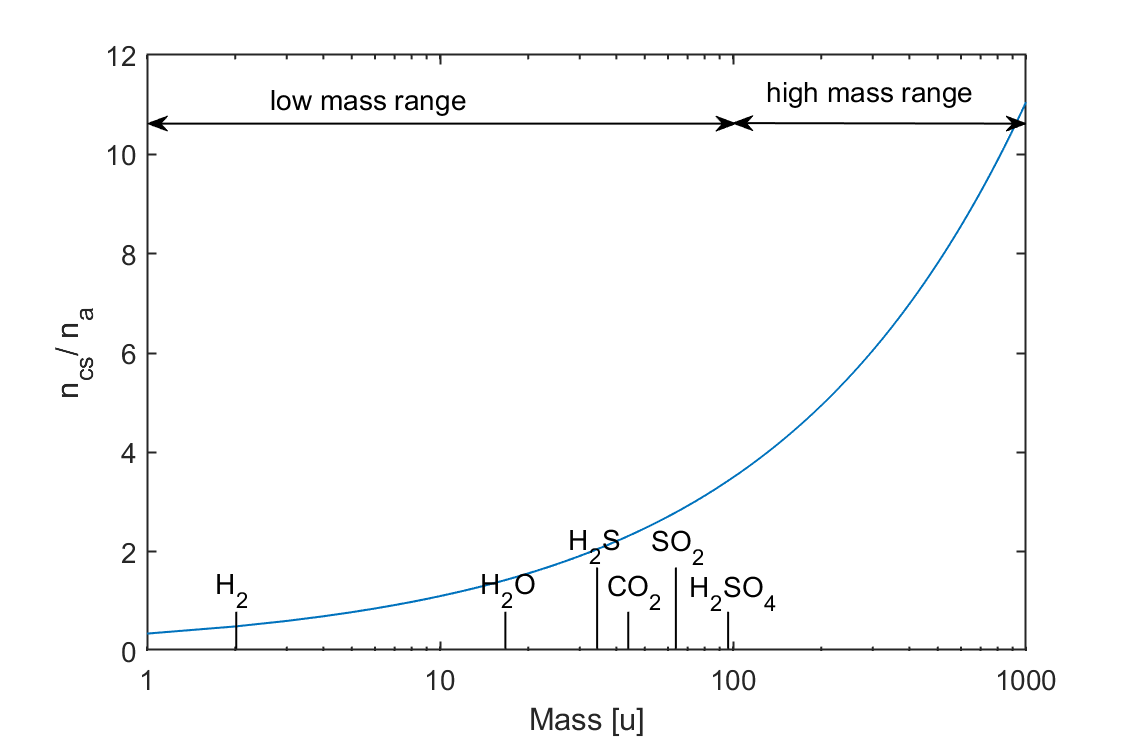
\includegraphics[width= .7\textwidth]{Bilder/mV1.png}
		\caption{Density enhancement $n_{cs}/n_a$ of the antechamber as a function of the particle mass $m$.}
		\label{th:densEnhm}
	\end{figure}
	\begin{figure}[h!] % velocity
		\centering
		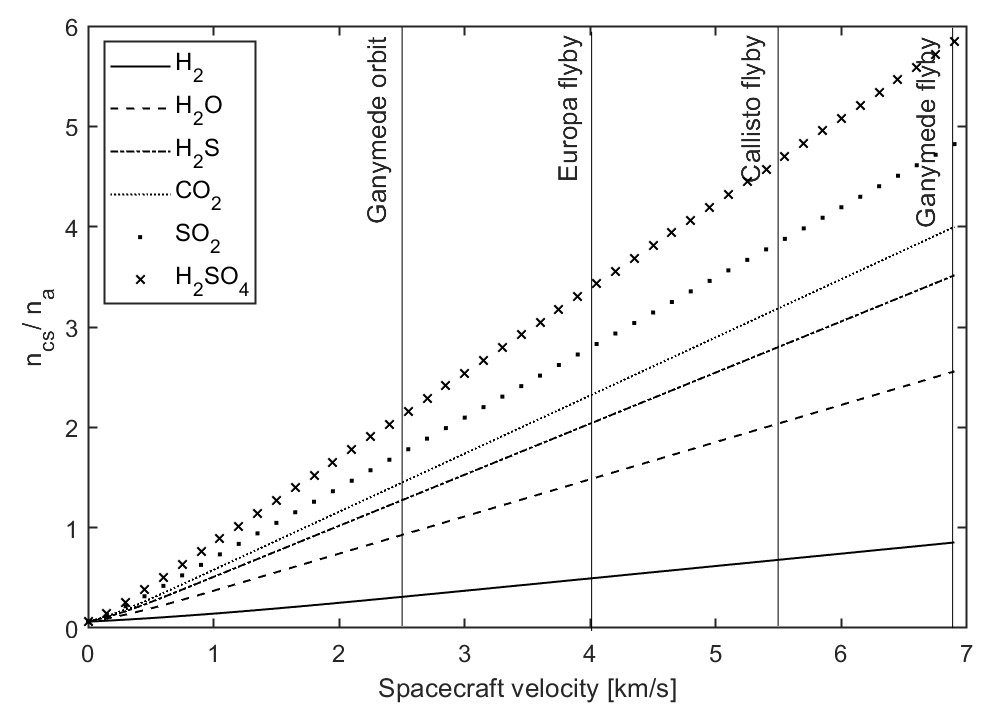
\includegraphics[width= .7\textwidth]{Bilder/velocityV1.png}
		\caption{Density enhancement $n_{cs}/n_a$ of the antechamber as a function of the spacecraft velocity $v_{sc}$ for different species expected in the icy moons exospheres.}
		\label{th:densEnhvelo}
	\end{figure}
	\begin{figure}[h!] % chi theat
		\centering
		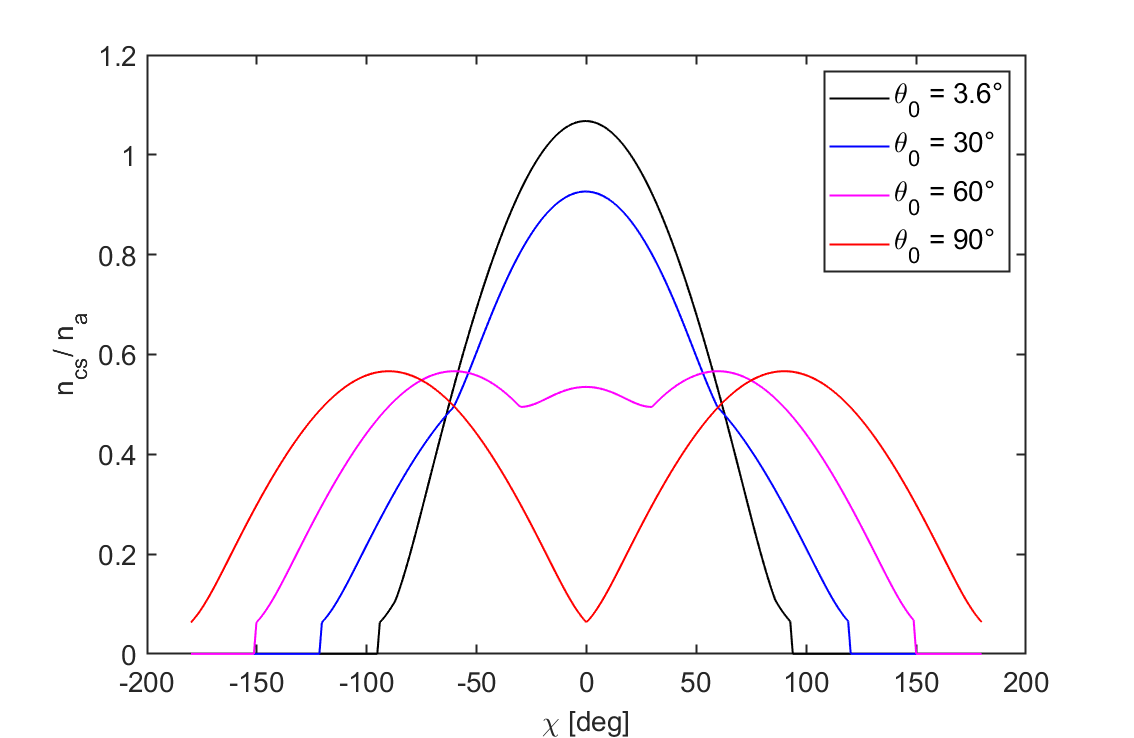
\includegraphics[width= .8\textwidth]{Bilder/Chi_theta0.png}
		\caption{Density enhancement $n_{cs}/n_a$ of the antechamber as a function of the angle $\chi$ between the gas inflow direction and the x-axis of the instrument for different positions of the two entrance holes $\theta_0$. $\theta_0=30\degree$ is the position of the holes in flight configuration.}
		\label{th:densEnhChiTheta}
	\end{figure}
	A small $\omega$ implies a big surface area with which the particles interact before being detected. The bigger the number of interactions is, the bigger is the influence of $k$. The $\omega$ of NIM's antechamber is about 5.06°, which is very small and therefore a small change in $k$ has a big impact on the density enhancement.\\
	Fig.~\ref{th:densEnhm} shows the density enhancement of the antechamber as a function of the particles unit mass~[u]. The figure shows that higher mass species have a higher density enhancement factor than low mass species. Since the higher mass species are usually of low abundance in the icy moons exospheres \cite{Vorburger2015,Vorburger_2018}, this mass dependence of the density enhancement factor is very helpful.\\
	Fig.~\ref{th:densEnhvelo} shows the density enhancement of the antechamber as a function of the spacecraft velocity for different species. We expect H\textsubscript{2}O and different radiolysis products such as H\textsubscript{2}, O\textsubscript{2} or HO in the icy moons' exosphere. Absorption lines in the near infrared recorded by the Near Infrared Mapping Spectrometer (NIMS) on board of the Galileo spacecraft indicate CO\textsubscript{2} bond to other solid materials in the soil. Sulphur is ejected by the Galilean moon Io and is therefore part of the Jupiter's plasma torus. The sulphur compounds are a result of the ion bombardment on the icy moons' surface. Sulphur reacts with water resulting in various different compounds such as sulphur dioxide (SO\textsubscript{2}) or sulphuric acid (H\textsubscript{2}SO\textsubscript{4}) \cite{Collins_2014}. Fig.~\ref{th:densEnhvelo} shows that with increasing flyby velocity, the particles get more amplified. Heavier species are stronger amplified than light ones as it was already shown in Fig.~\ref{th:densEnhm}.\\
	Fig.~\ref{th:densEnhChiTheta} shows the density enhancement of the antechamber as a function of different particle influx angles $\chi$. $\chi$ is measured in the x-/y-~plane of NIM's coordinate system (see Fig.~\ref{fig:thAntIs}). The function was evaluated for different positions of the entrance holes. The minimal angle the two entrance holes can be apart from each other without overlapping is 3.6\si{\degree}. The holes of the PFM antechamber are at $\theta_0 = \pm30~\si{\degree}$. With that configuration the biggest signal intensity is measured with a spacecraft ramp direction of 0\si{\degree}. When the two holes are at $\pm$60\si{\degree} the intensity distribution has a plateau between $\pm$60~\si{\degree} and also a wider angular range. 
	\pagebreak
	This is an interesting feature under certain circumstance. For NIM it is unnecessary because the spacecraft blocs the field of view (FoV) for angles bigger than 100\degree~(see also Chap.~\ref{subsubsec:Calfly}).
	
	
%-------------------------------------------------------------------------------------------		
	\subsection{Field-of-View Analysis}\label{subsubsec:Calfly}

	In the following section, the fourth Callisto flyby of JUICE according to the Consolidated Report on Mission Analysis (CReMA) version 3.2 trajectory 141a \cite{SOC_Crema3p2} is analysed as an example of the expected particle flux directions during a flyby. Fig.~\ref{fig:FlybyCal1852}~-- Fig.~\ref{fig:FlybyCal1957} show the changing FoV orientation of the NIM instrument at different times. The reference coordinate system for these graphics is the ecliptic coordinate system. During the flyby, the spacecraft changes its orientation leading to a different appearance of the objects in the figures. The centres of the entrance holes of the antechamber are marked as blue circles, the FoVs of the entrance 
		\begin{figure}[h!]
		\centering
		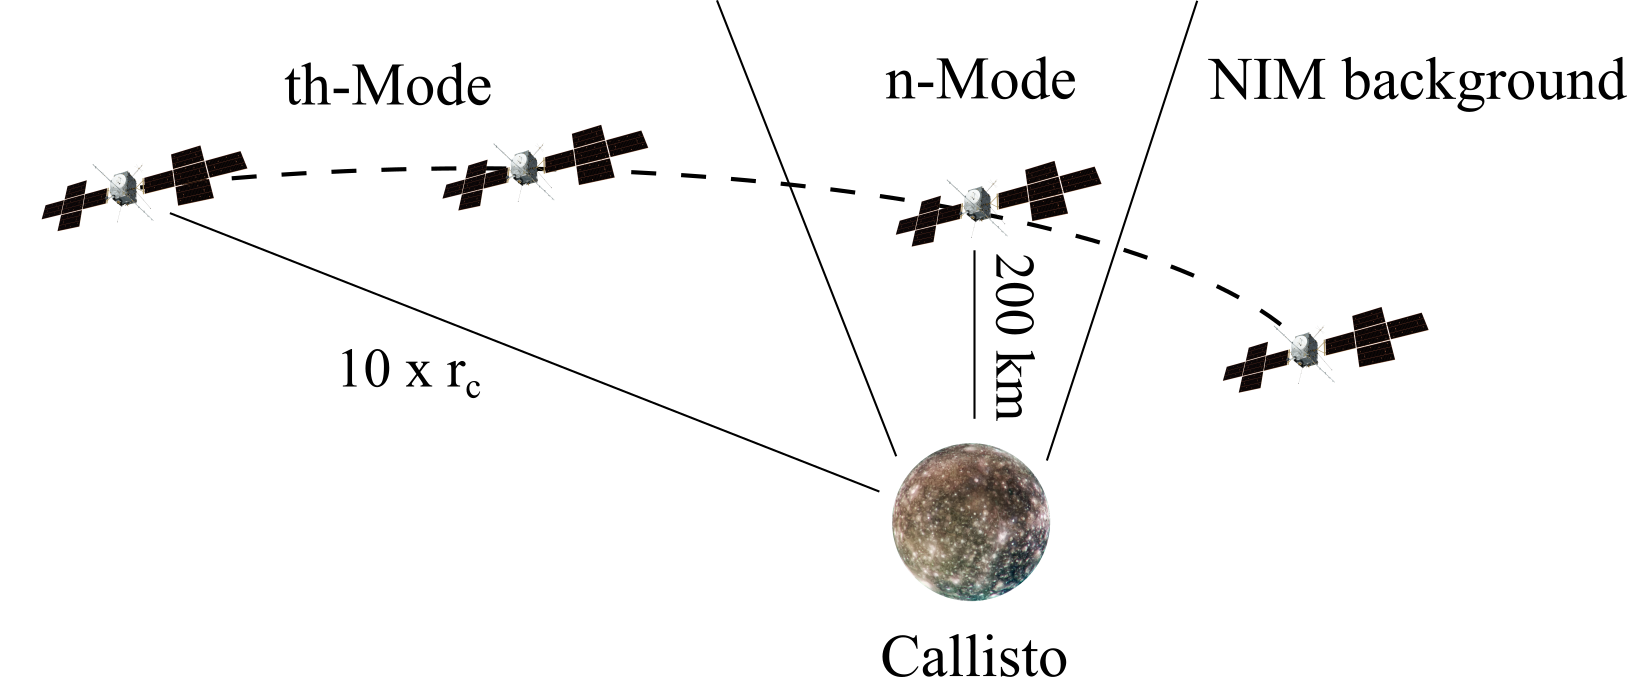
\includegraphics[width=.8\textwidth]{Bilder/Callisto_flyby_schematic.png}
		\caption{Schematics of the operation during a flyby at Jupiter's moon Callisto.}
		\label{fig:CalflybySchem}
	\end{figure}
	\begin{figure}[h!]
		\centering
		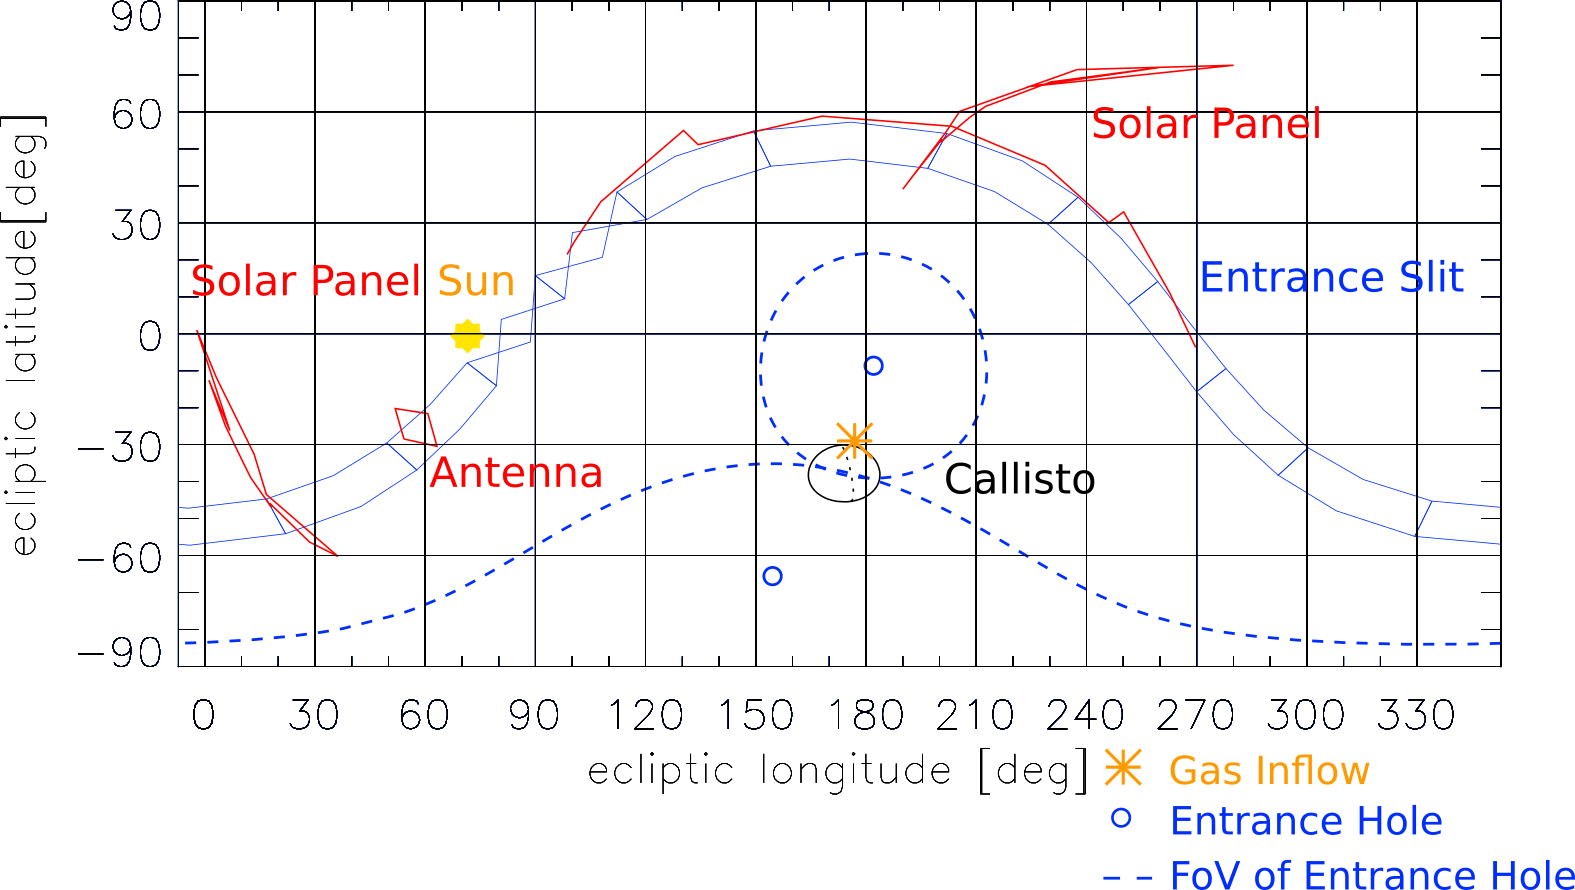
\includegraphics[width = .7\textwidth]{Bilder/NIM_pointing_2031JAN15185200.png}
		\caption{Full-sky map as viewed from NIM during the fourth Callisto flyby based on calculation of CReMA~3.2 trajectory~141a \cite{SOC_Crema3p2} 1~h before closest approach 15'600~km above Callisto's surface.}
		\label{fig:FlybyCal1852}
	\end{figure}
	\begin{figure}[h!]
		\centering
		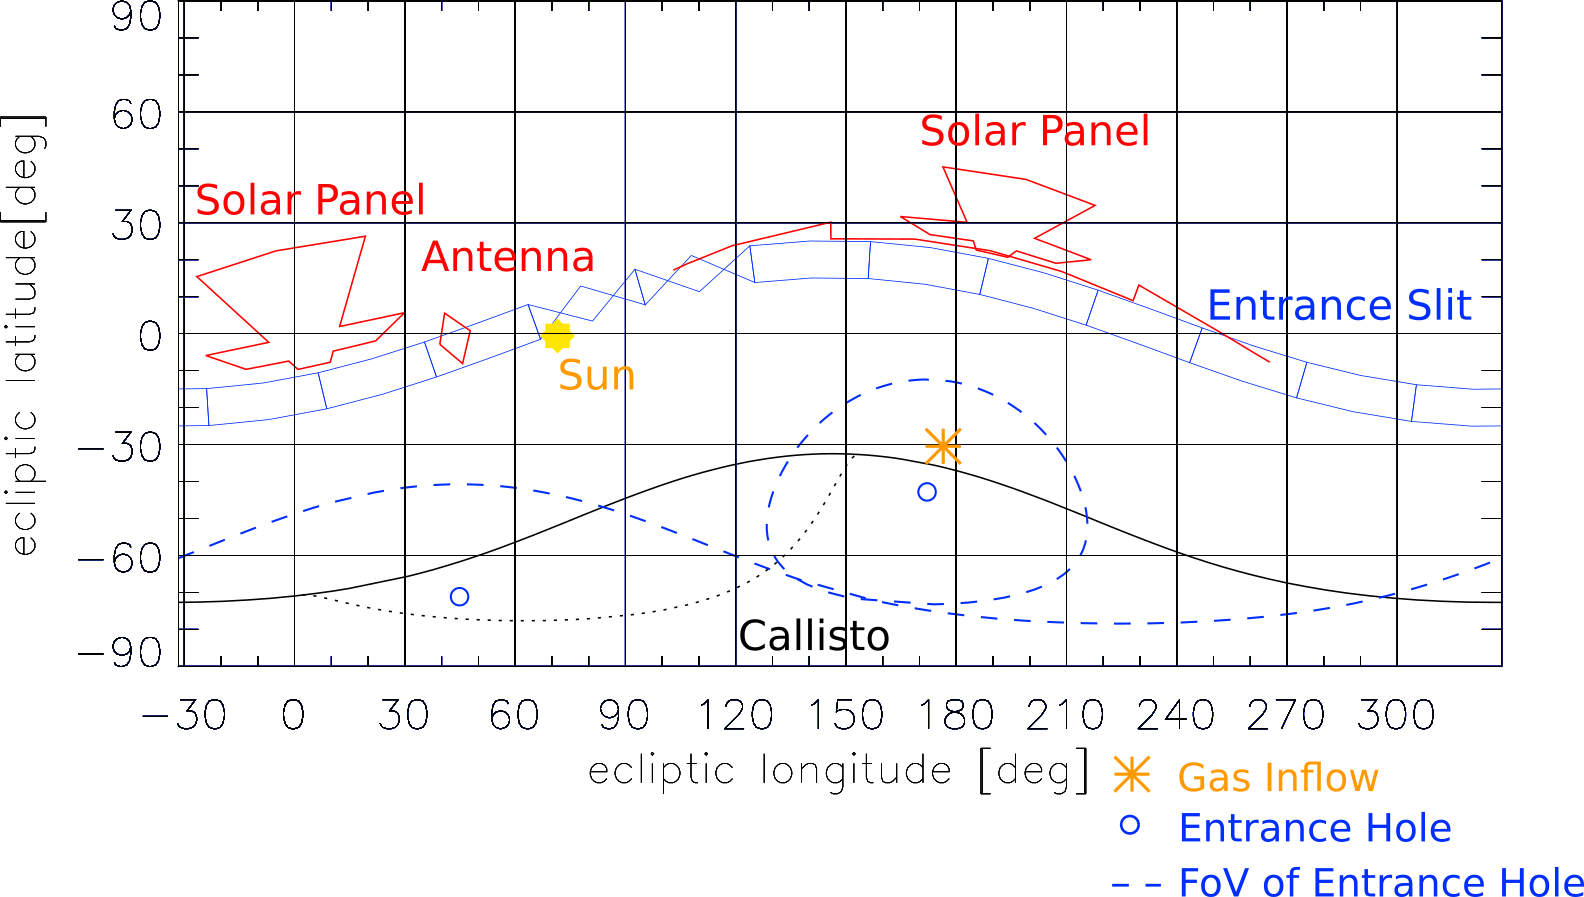
\includegraphics[width = .7\textwidth]{Bilder/NIM_pointing_2031JAN15194200.png}
		\caption{Full-sky map as viewed from NIM during the fourth Callisto flyby based on calculation of CReMA~3.2 trajectory~141a \cite{SOC_Crema3p2} 10~min.\ before closest approach 1'560~km above Callisto's surface.}
		\label{fig:FlybyCal1942}
	\end{figure}
	\begin{figure}[h!]
		\centering
		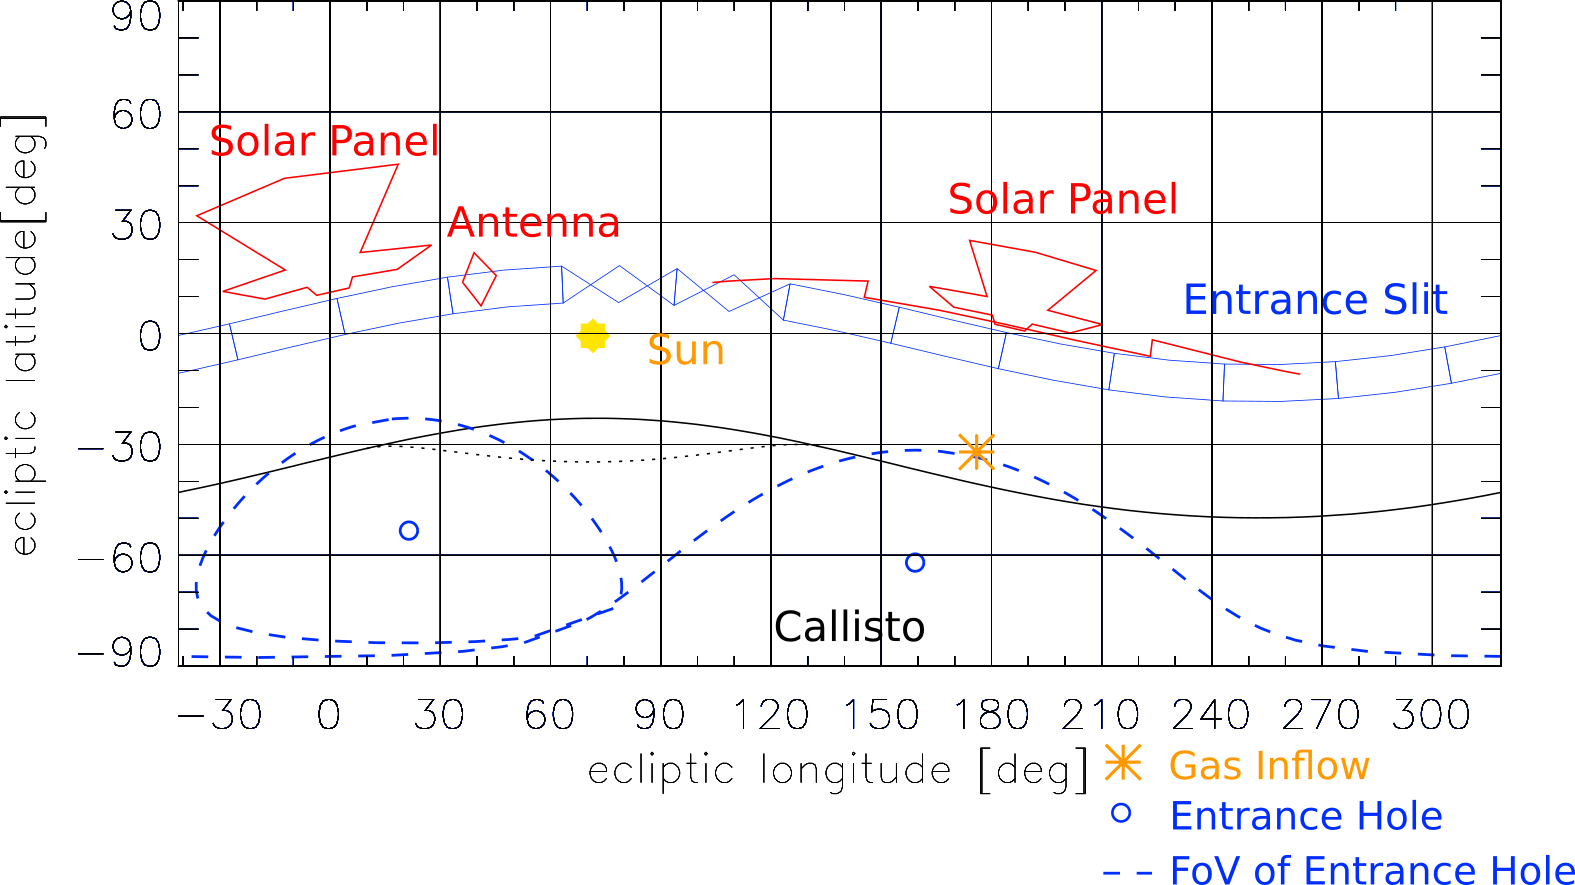
\includegraphics[width = .7\textwidth]{Bilder/NIM_pointing_2031JAN15194700.png}
		\caption{Full-sky map as viewed from NIM during the fourth Callisto flyby based on calculation of CReMA~3.2 trajectory~141a \cite{SOC_Crema3p2} 5~min.\ before closest approach 580~km above Callisto's surface.}
		\label{fig:FlybyCal1947}
	\end{figure}
	\begin{figure}[h!]
		\centering
		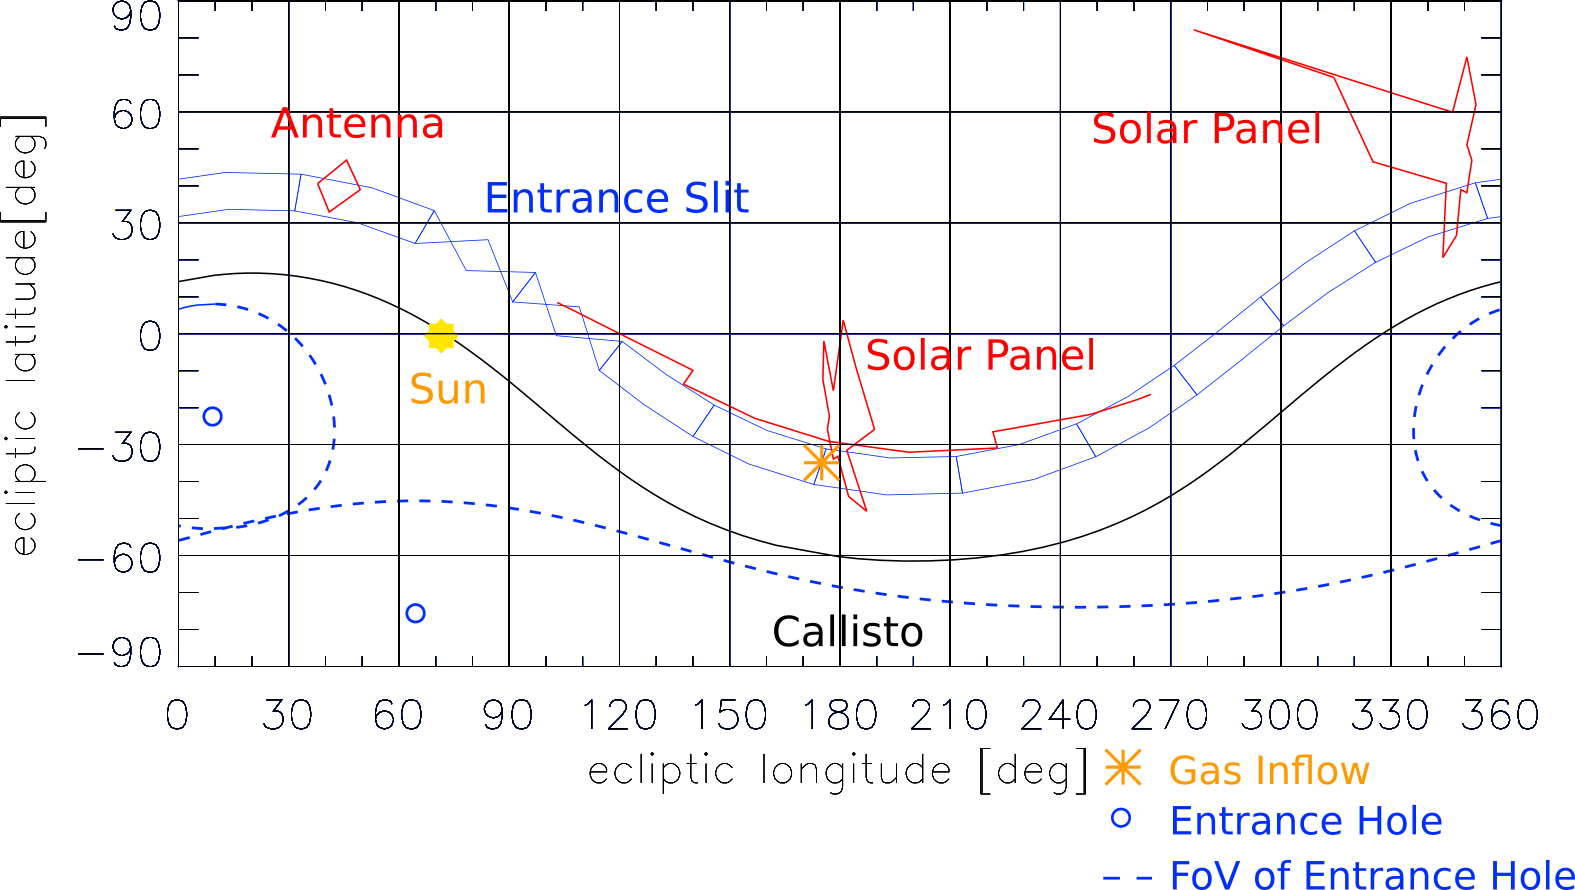
\includegraphics[width = .7\textwidth]{Bilder/NIM_pointing_2031JAN15195200_tilt.png}
		\caption{Full-sky map as viewed from NIM during the fourth Callisto flyby based on calculation of CReMA~3.2 trajectory~141a \cite{SOC_Crema3p2} closest approach 200~km above Callisto's surface with the spacecraft solar panels oriented toward the Sun to maximises power generation.}
		\label{fig:FlybyCal1952sol}
	\end{figure}
	\begin{figure}[h!]
		\centering
		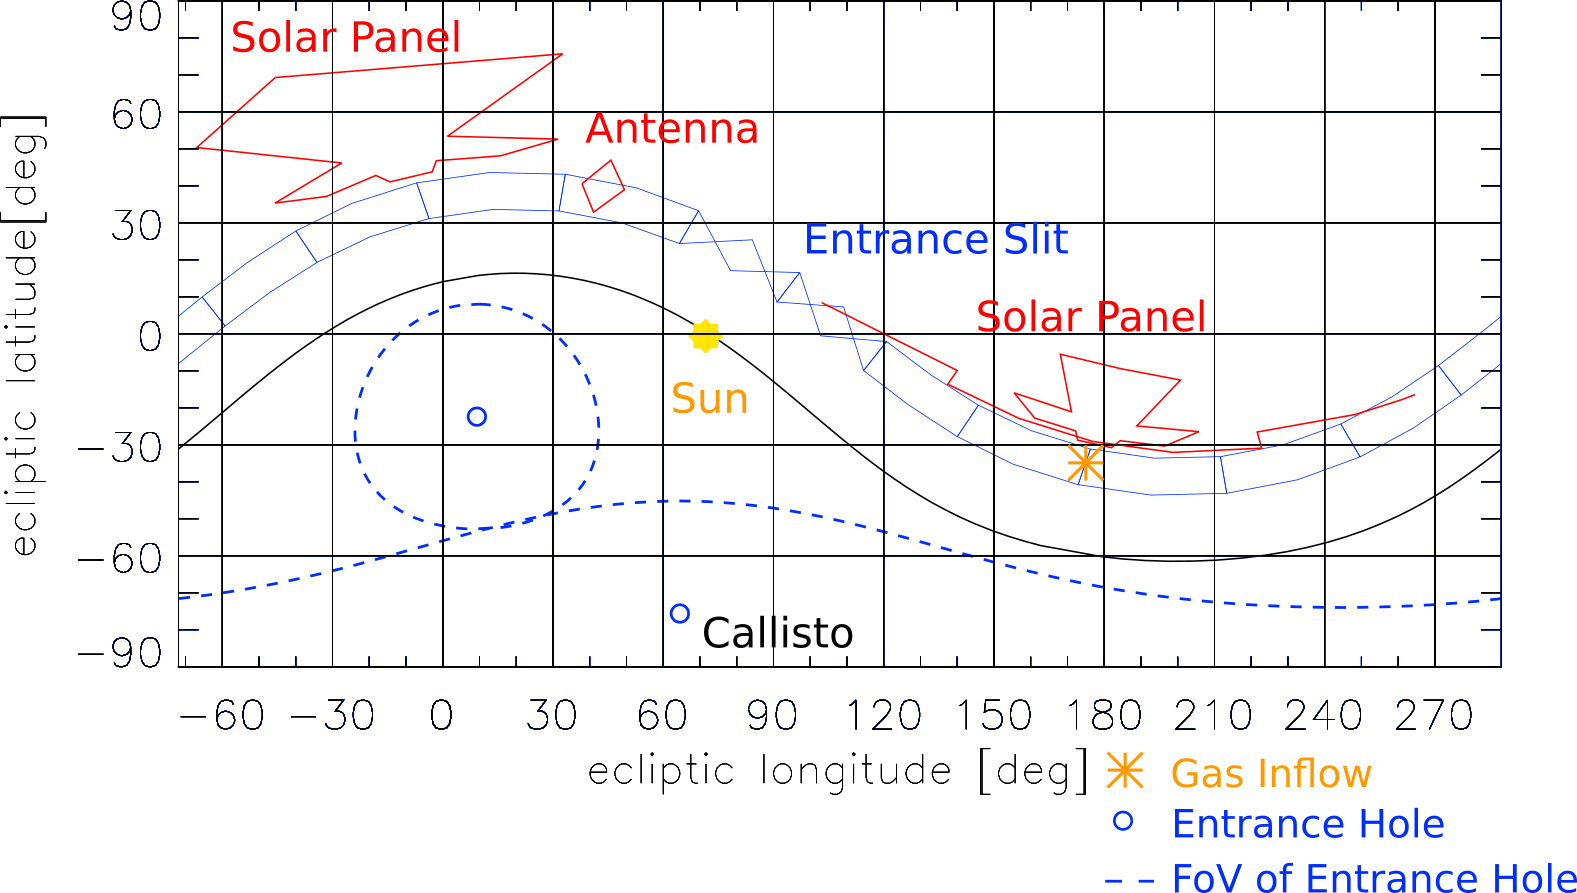
\includegraphics[width = .7\textwidth]{Bilder/NIM_pointing_2031JAN15195200.png}
		\caption{Full-sky map as viewed from NIM during the fourth Callisto flyby based on calculation of CReMA~3.2 trajectory~141a \cite{SOC_Crema3p2} closest approach 200~km above Callisto's surface with solar panels tilted to leave unobstructed NIM's field-of-view of the n-Mode.}
		\label{fig:FlybyCal1952}
	\end{figure}
	\begin{figure}[h!]
		\centering
		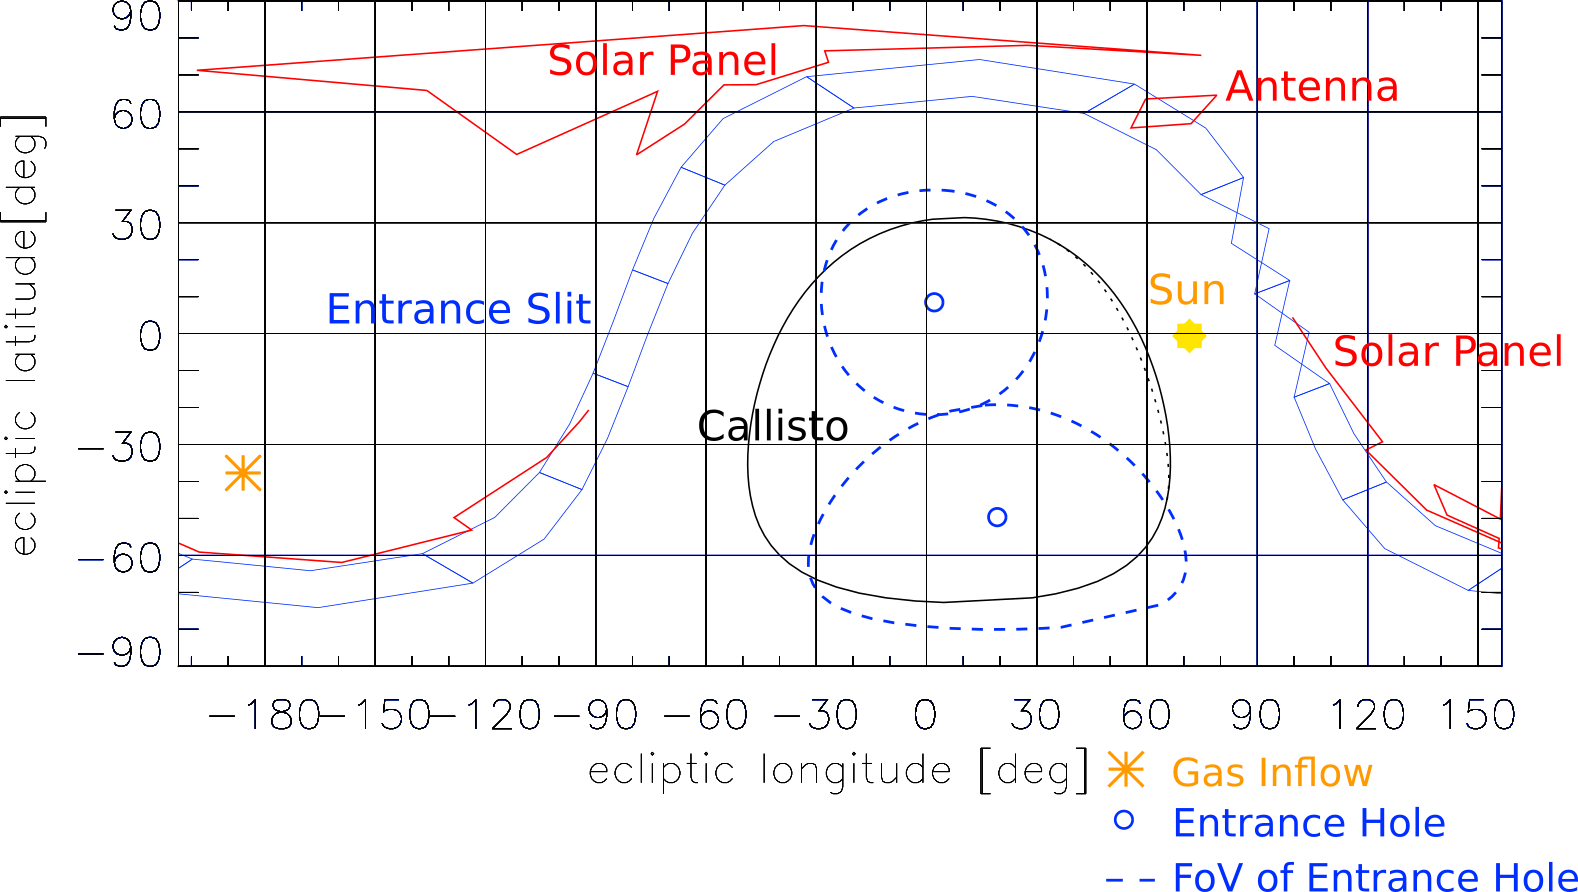
\includegraphics[width = .7\textwidth]{Bilder/NIM_pointing_2031JAN15195700.png}
		\caption{Full-sky map as viewed from NIM during the fourth Callisto flyby based on calculation of CReMA~3.2 trajectory~141a \cite{SOC_Crema3p2} 5~min.\ after closest approach 640~km above Callisto's surface.}
		\label{fig:FlybyCal1957}
	\end{figure}
	\begin{figure}[h!]
		\centering
		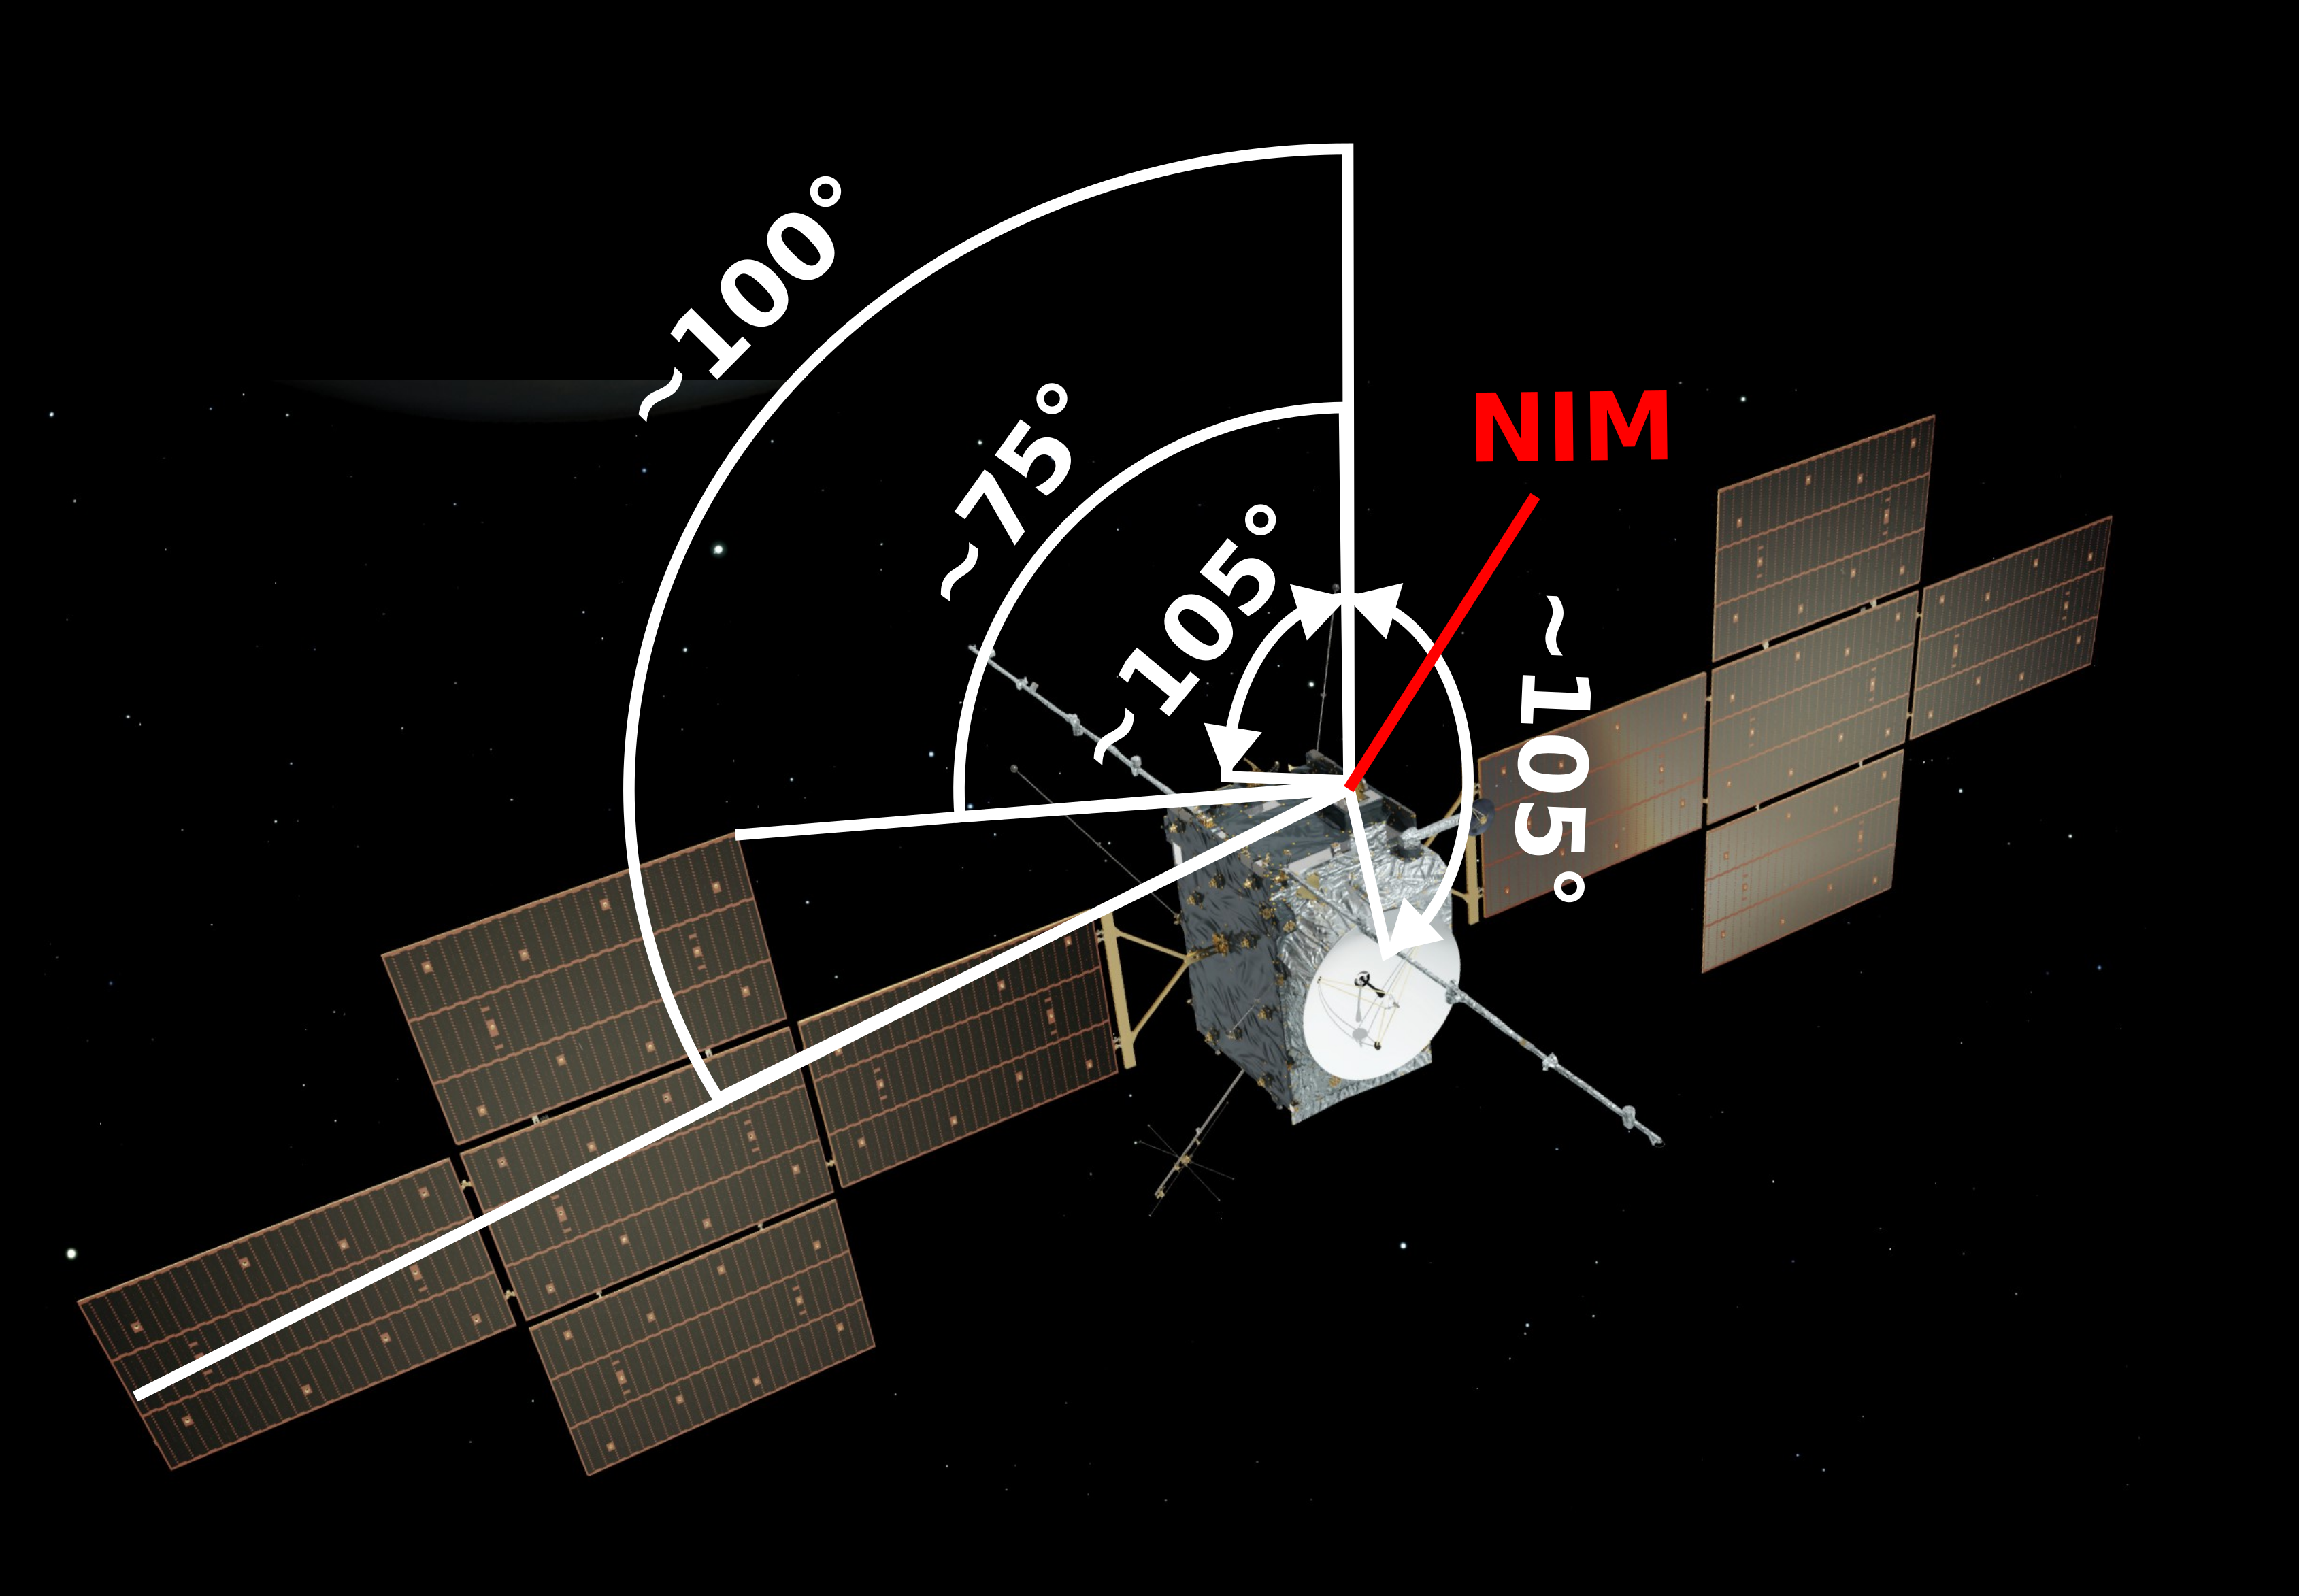
\includegraphics[width=.6\textwidth]{Bilder/SC_Angle.png}
		\caption{NIM field-of-View on the JUICE spacecraft.}
		\label{fig:SCFoV}
	\end{figure}
	holes of the antechamber are marked as dashed blue lines (actually, the 30° radius line of the FoV), the entrance slit at the open source entrance is the blue, striped band with the sinusoidal shape. The solar panels and the rim antenna of the spacecraft are marked in red. The gas inflow direction is marked as an orange asterisk. Fig.~\ref{fig:FlybyCal1852} shows the FoV orientation 1~h before closest approach 15'600~km above Callisto's surface. The gas inflow direction is in between the two entrance holes of the antechamber thus both holes collect gas from Callisto's exosphere. As the spacecraft moves closer to the moon, the gas inflow direction moves towards the entrance slit. 5~min. before closest approach, NIM changes from thermal to neutral mode because of the narrow FoV of 10° width of the entrance slit and the short time window during which the gas inflow direction is within the FoV of the entrance slit (Fig.~\ref{fig:FlybyCal1947}). At this time, the gas inflow direction is still in the FoV of the antechamber. The design goal for the switch over between the two modes is 1~s to minimise the number of lost measurements due to this mode change. These measurements are very crucial because the closer the spacecraft gets to the moon's surface, the higher is the exospheric density and therefore the signal intensity (see Fig.~\ref{fig:VorburgIc2015}). 5~min. after closest approach, the gas inflow direction is below the FoV of the neutral gas channel and NIM takes background measurements (Fig.~\ref{fig:FlybyCal1957}). In addition, the spacecraft structure obstructs angles higher than 105° either by the platform on which NIM is mounted or by the solar panels \cite{NIM_FoV}. Fig.~\ref{fig:SCFoV}) shows the JUICE spacecraft with the solar panels in straight up position where they limit NIM's FoV to 75° in the direction along the solar panels. When the solar panels are tilted by 90°, they obstruct NIM's FoV for angles bigger than 100° which is configuration of the closest approach when NIM is measuring with the neutral gas channel. When gas strikes the spacecraft is sputters particles from the spacecraft's surface. NIM is not able to determine if these particles are part of the moons exosphere or if they originate from the spacecraft. In general, the solar panels are adjusted perpendicular to the Sun where possible to maximise power generation. 10~min. before closest approach, the solar panels are tilted to leave the FoV of NIM unobstructed to measure with the neutral gas mode. In case the solar panels would stay perpendicular to the Sun, the gas would graze the surface of the solar panel as it is shown in Fig.~\ref{fig:FlybyCal1952sol}. Fig.~\ref{fig:FlybyCal1952} shows the same scenario but with the solar panels tilted to leave NIM's FoV unobstructed for the neutral gas channel.\\
	Fig.~\ref{fig:densEnhChiFlyby} shows the density enhancement of the antechamber with the total FoV of the two entrance holes marked as red area $\pm$30\degree around the position of the two entrance holes. The orange asterisks mark the gas inflow direction for the various scenarios mentioned above. Depending on the flyby, the main gas inflow direction is from the $+\chi$ or $-\chi$ side. Therefore, it was decided to make two entrance holes in the antechamber to allow measurements with angles different to the main direction to enlarge the FoV of the antechamber. The holes should also not be too close at the entrance because structures of the spacecraft bloc angles bigger than 105° and the density enhancement at such big angles would be useless.\\
	Fig.~\ref{fig:VorburgIc2015} shows simulated density profiles of Callisto's exosphere. In this model, the particles have been sublimated from Callisto's ice surface at the sub-solar point \cite{Vorburger2015}. The x-axis at the bottom shows the height above the exobase and the x-axis at the top shows the time before closest approach of the spacecraft. The orange areas are density distributions NIM is not able to detect. For the flyby discussed above, the closest approach of the spacecraft is at 200~km above Callisto's surface. The detection limit of NIM in Jupiter's strong radiation environment is 4~cm\textsuperscript{--3} for an integration time of 5~sec \cite{Lasi_2017_Detector}. 5~min before closest approach, NIM changes from thermal to neutral mode indicated with the small orange bar at position 5~min. During the mode change, NIM cannot record any spectra. The longer the switch over takes, the bigger is therefore this area where precious spectra get lost.\\
	\begin{figure}[H]
		\centering
		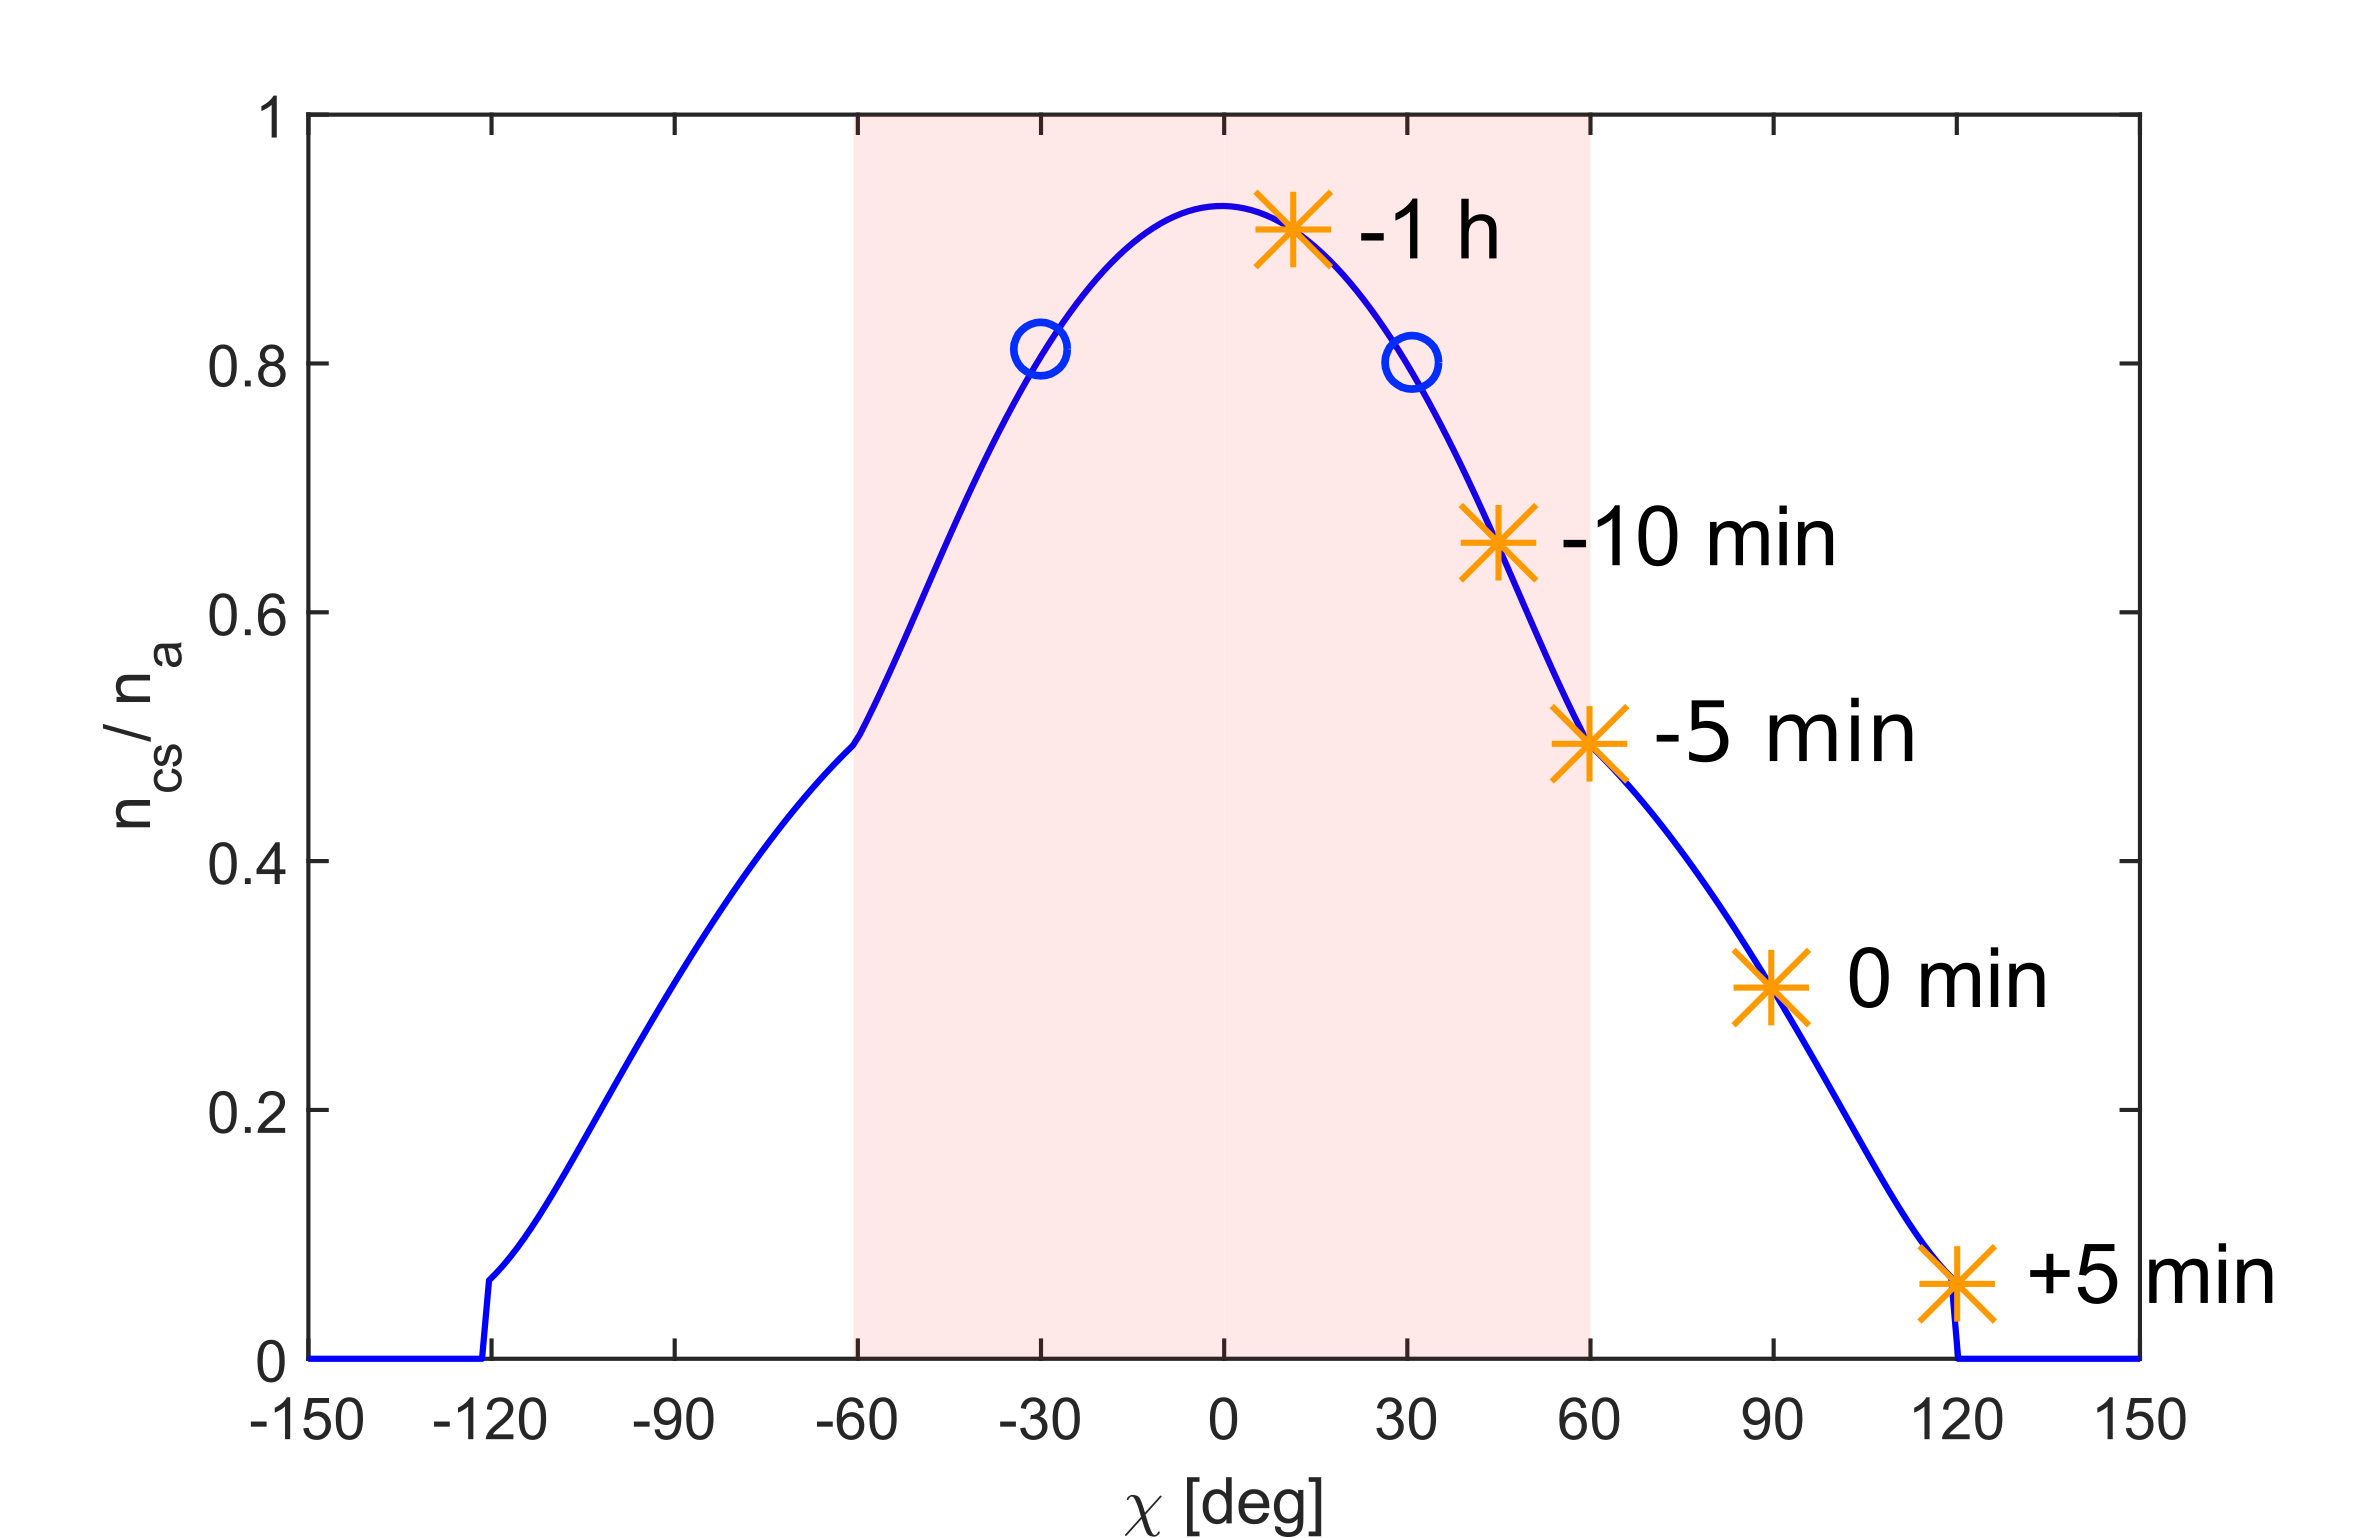
\includegraphics[width=.8\textwidth]{Bilder/Chi_theta0_flyby.png}
		\caption{Density enhancement $n_{cs}/n_a$ of the antechamber as a function of the angle $\chi$ between the gas inflow direction and the x-axis of the instrument for different positions of the two entrance holes $\theta_0$. The blue circles mark the entrance hole positions and the red area marks the FoV. The asterisks mark the gas influx direction from 1~h before until 5~min.\ after closest approach of CReMA~3.2 trajectory 141a \cite{SOC_Crema3p2}.}
		\label{fig:densEnhChiFlyby}
	\end{figure}
	\begin{figure}[h!]
		\centering
		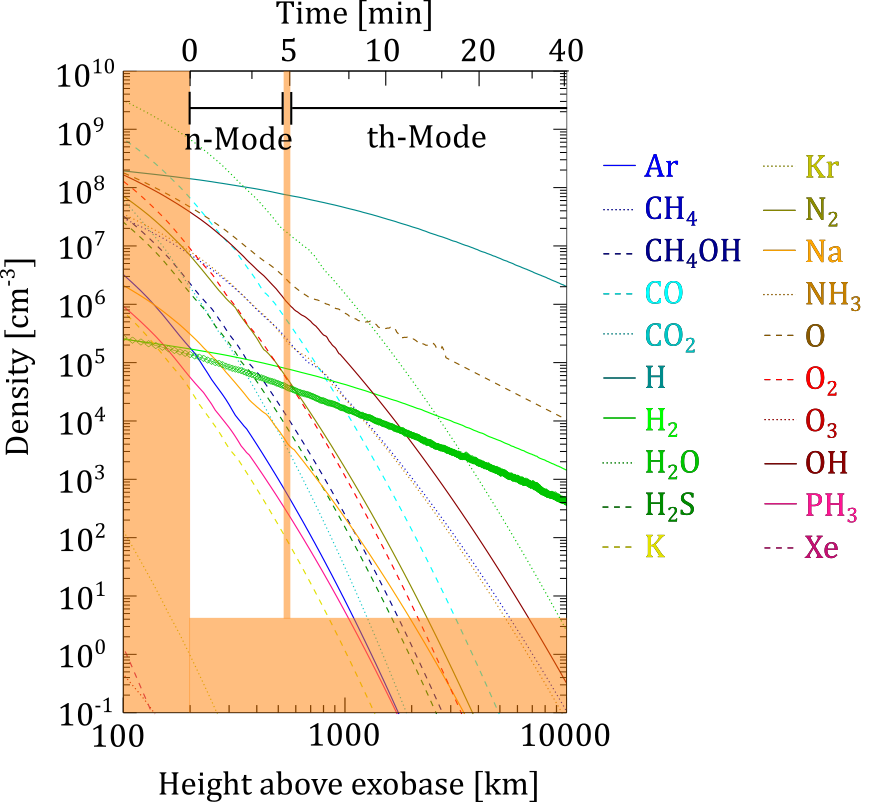
\includegraphics[width=.7\textwidth]{Bilder/Vorburger_Icarus_2015.png}
		\caption{Gas density profiles of Callisto's exosphere simulated by Vorburger et al. \cite{Vorburger2015}. Orange areas mark regions NIM is not able to detect any species either because the JUICE spacecraft does not fly closer to the moon's surface or due to the detection limit of the NIM instrument.} % 4~cm\textsuperscript{--3}
		\label{fig:VorburgIc2015}
	\end{figure}
	NIM has different measuring modes with regards to the recording configuration of the spectra. One of these configuration parameters is the integration time. The integration time is the time during which the instrument sums up all recorded single spectra. With a pulse frequency of 10~kHz, a spectrum with an integration time of 5~sec consists of 50'000 summed up single spectra. The SNR increases with the square root of the integration time because the random noise only grows with the square root of the integration time and the gas peaks grow proportionally because they appear always at the same position in the spectrum. Therefore, a longer integration time improves the SNR and the amount of acquired data per time is smaller, which is an advantage because JUICE can only transmit a certain amount of data per day back to Earth. A longer integration time also implies a worse spacial resolution of the density profile along the flight path of the spacecraft because the sampling rate is lower.\\
	For a flyby, 12~h before closest approach at the moons, NIM will start with a bake out and warm up of the system to get the system in a stable thermal state. The bake out is necessary to get rid of condensed particles at the instrument. Otherwise, these particles are released during operation of the instrument and are then visible in the recorded mass spectra. These particles cannot be distinguished from particles originating from the moons' exospheres.\\
	The integration time can be set to 1, 5, 10, 100 or 300~seconds. When the spacecraft is far away from the moon (11~h before closest approach), the integration time is set to 300~sec because at these far distances the neutral particle density is very low and therefore a longer integration time is favourable because it corresponds to a higher SNR. In addition, spacial resolution is of minor importance at these distances. When JUICE gets closer to the moon, the integration time is decreased because the neutral particle number density increases and to get a better picture from the spacial distribution of gas composition in the icy moons' exosphere. At closest approach for the flybys at Ganymede and Callisto, the integration time is about 5~sec. To reduce the amount of produced data, NIM records most of the time spectra with a reduced mass range which records masses between 0--300~u. For the two Europa flybys, the recorded mass range will be 0--1000~u because there the main focus lies on the detection of potential organic compounds. As a trade-off the minimal integration time will be set to 10~sec.\ instead of 5~sec.\ as for the flybys at Ganymede and Callisto. This on one hand results in an increased sensitivity but on the other hand, the spacial resolution is then worse for these flyby. The Galileo spacecraft recorded plumes of water vapour on Europa. JUICE would like to fly through one these plumes and therefore, NIM has a special plume mode where the integration time is only 1~sec to get a good spacial resolution of the plume. since the signal is expected to be high in the plume SNR should be good.
	
	% Particle density for Europa is 1.515 (10 sec integration time, better SNR, bigger mass range, lower spacial resolution (Euro (4 km/s) Callisto (5.5 km/s in average depending on the flyby) 4 km/s with 10 sec = 1 data point evey 40 km)), for Callisto 4 (5 sec integration time, worse SNR, lower mass range, better spacial resolution with 20 km per data point)
	
%------------------------------------------------------------------------------------------
	\subsection{Shutter Performance} \label{subsubsec:motorflow}
	With the open-source entrance, NIM is able to measure neutral particles and ions directly without any interaction with the structure. Since the n-mode and the th-mode use the same ion-source, NIM has a shutter to close the passage between to the antechamber and the ionisation region. This shutter is mounted between the ionisation region and the antechamber (Fig.~\ref{fig:shutterMotor}~left). When the shutter is open, the gas flows from the antechamber right through the hole into the ionisation region. When the shutter is closed, the hole in the shutter moves to the side as it is indicated in Fig.~\ref{fig:shutterMotor} right panel. The shutter does not close the hole perfectly and therefore 
	\begin{figure}[h!]
		\begin{subfigure}{0.5\textwidth}
			\centering
			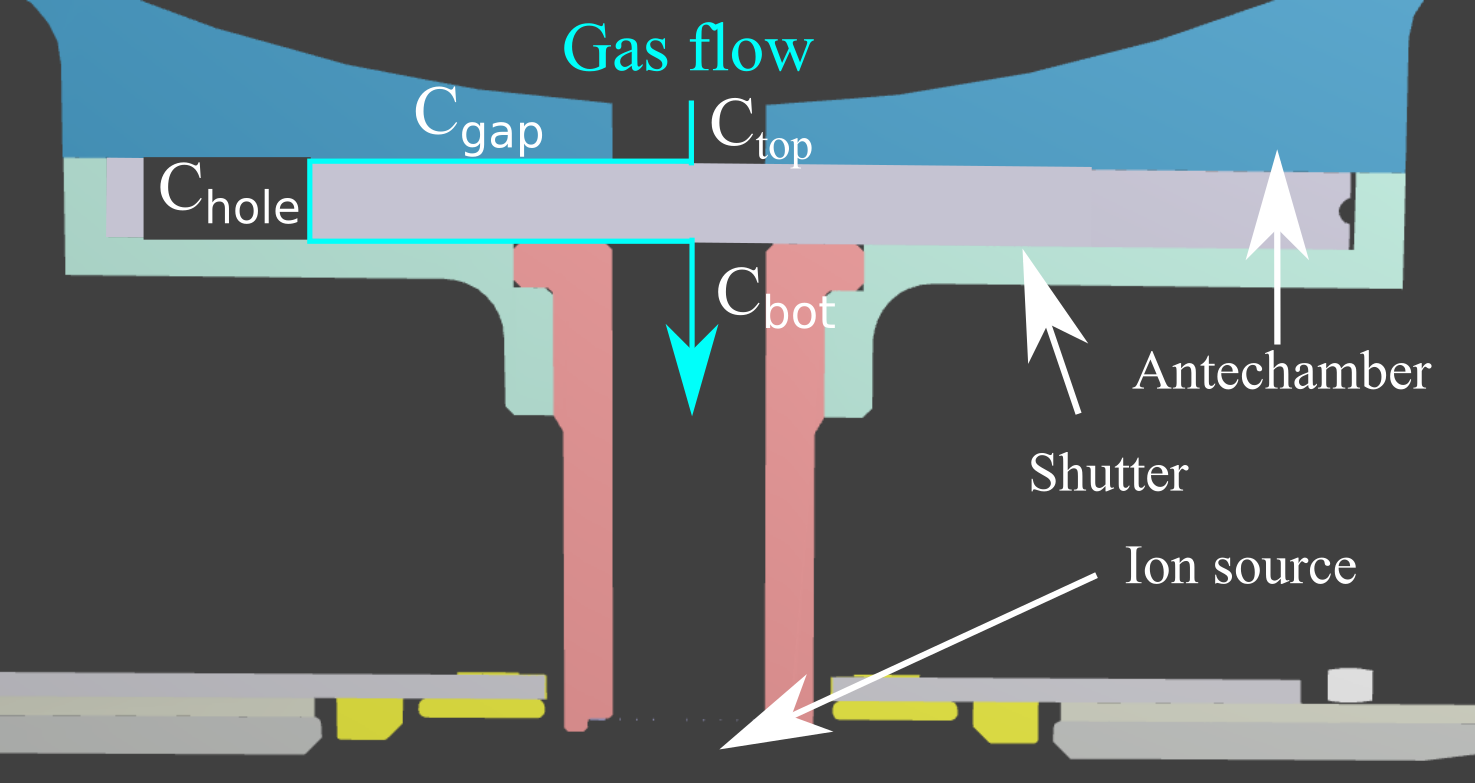
\includegraphics[width=\textwidth]{Bilder/Shutter_sideview.png}
		\end{subfigure}
		\begin{subfigure}{0.5\textwidth}
			\centering
			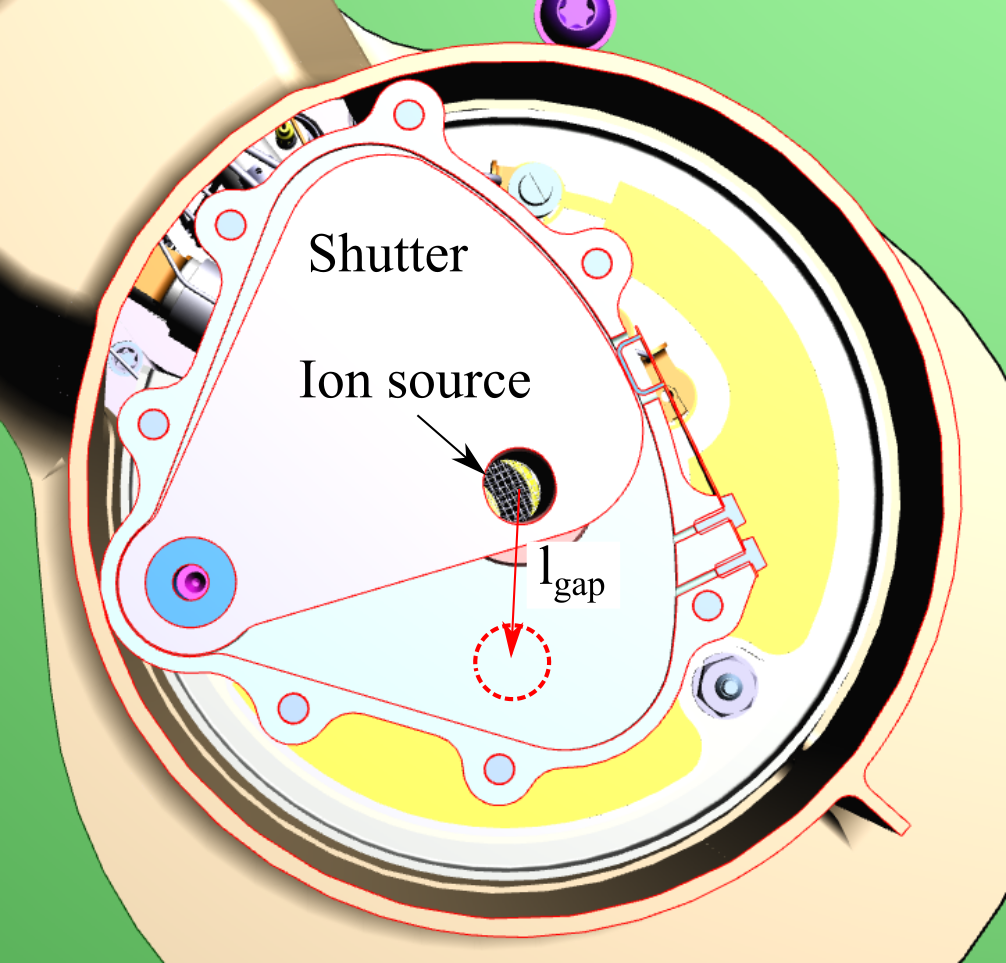
\includegraphics[width=.8\textwidth]{Bilder/Shutter_topview.png}
		\end{subfigure}
		\caption{Left: side view when shutter is closed. Right: Top view with open shutter. When the shutter is closing, the central hole of the shutter blade moves to the red position.}
		\label{fig:shutterMotor}
	\end{figure}
	a small amount of gas flows through the gap around the shutter into the ionisation region. In the following section, the molecular flow conductance of the closed shutter is determined. The molecular flow conductance $C$ is:
	\begin{equation}
		C = \frac{A\cdot\bar{v}\cdot a}{4}
	\end{equation}
	With $A$ the cross-section of the tube connecting the antechamber and the ionisation region, $\bar{v}$ the average velocity of the thermalised gas flowing through the opening and the transmission probability $a$ depending on the length-to-diameter ratio of the tube (Eq.~\eqref{eq:MolFloConFitFunc}). When the shutter is closed, the conductance of the tube $C_{tot}$ is divided into four terms: The conductance of the upper part of the tube $C_{top}$, the conductance of the gap between the shutter blade and the pocket $C_{gap}$, the conductance of the hole in the shutter $C_{hole}$ and the conductance of the lower part of the tube connecting the antechamber with the ionisation region $C_{bot}$ (Fig.~\ref{fig:shutterMotor}~left):
	\begin{align}
		C_{top}  &= \frac{r_{aIs}^2\cdot\pi\cdot\bar{v}\cdot a_{top}}{4}\\
		C_{gap}  &= \frac{2\cdot r_{aIs}\cdot \pi \cdot h_{gap}\cdot\bar{v}\cdot a_{gap}}{4}\\
		C_{hole} &= \frac{r_{aIs}^2\cdot\pi\cdot\bar{v}\cdot a_{hole}}{4}\\
		C_{bot}  &= \frac{r_{aIs}^2\cdot\pi\cdot\bar{v}\cdot a_{bot}}{4}
	\end{align}
	\begin{table}[H]
		\begin{center}
			\begin{tabular}{|l r| l r| }
				\hline
				$a_{top}$	& 0.73 	& $h_{top}$		& 1.5~mm	\\
				$a_{gap}$	& 0.07 	& $h_{gap}$		& 0.01~mm \\
				$a_{hole}$ 	& 0.67 	& $h_{hole}$ 	& 2~mm\\
				$a_{bot}$ 	& 0.28 	& $h_{bot}$ 	& 12~mm\\
				$r_{aIs}$ 	& 2~mm & $l_{gap}$ 	& 7~mm\\
				\hline
			\end{tabular}
		\end{center}
		\caption{Nominal transmission probabilities $a$, tube heights $h$, tube radius $r_{aIs}$ and minimal gap length $l_{gap}$ when the shutter between the antechamber and the ionisation region is closed.}
		\label{tab:thMolFloConMotClosPara}
	\end{table}
	With $a_{top}$, $a_{gap}$, $a_{hole}$ and $a_{bot}$ the transmission probabilities of the different sections (Eq.~\eqref{eq:MolFloConFitFunc}) and $h_{top}$, $h_{gap}$, $h_{hole}$ and $h_{bot}$ the height of the different sections. $r_{aIs}$ is the radius of the tube connecting the antechamber with the ionisation region and $l_{gap}$ is the minimal distance between the hole in the shutter and the tube connecting the antechamber with the ionisation region. The nominal values for these parameters are listed in Table~\ref{tab:thMolFloConMotClosPara}. The average velocity $\bar{v}$ cancels out during the derivation of the geometry factor. The molecular flow conductance of the tube when the shutter is closed $C_{tot}$ is:
	\begin{equation}
		\frac{1}{C_{tot}} = \frac{1}{C_{top}} + \frac{2}{C_{gap}} + \frac{1}{C_{hole}} + \frac{1}{C_{bot}}
	\end{equation}
	\begin{figure}[H]
	\centering
		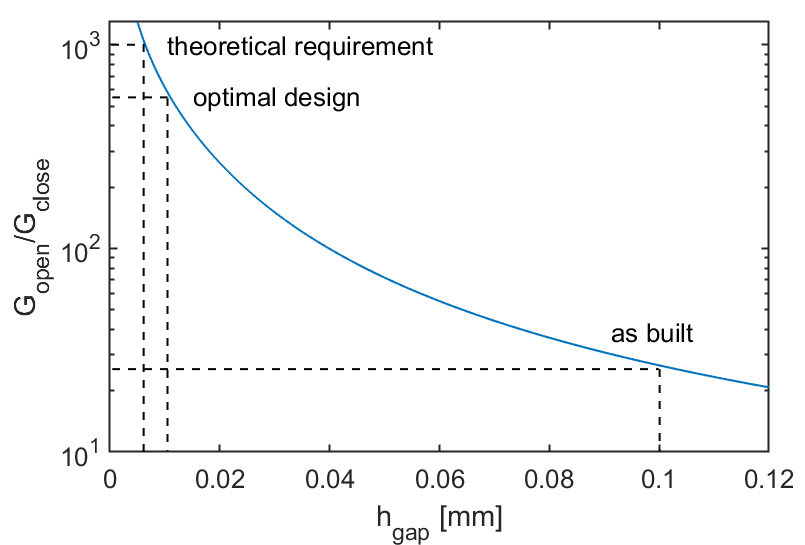
\includegraphics[width=.8\textwidth]{Bilder/Motor_1p2mm.png}
		\caption{Damping factor $G_{open}/G_{close}$ of the shutter as a function of the gap size $h_{gap}$ of the gap between the shutter and antechamber.}
		\label{fig:ShutGapSizeSigDamp}
	\end{figure}
	The conductance of one of the entrance holes of the antechamber is:
	\begin{equation}
		C_{aHi} = \frac{r_{aHi}^2\cdot\pi\cdot\bar{v}}{4}
	\end{equation}
	The geometry factor of the tube when the shutter is closed $G_{close}$ is:
	\begin{equation}
		G_{close} = \frac{C_{tot}}{C_{tot} + 2\cdot C_{aHi}}
	\end{equation}
	The geometry factor for the tube when the shutter is open was calculated with Eq.~\eqref{eq:geoOpenTube}. Fig.~\ref{fig:ShutGapSizeSigDamp} shows the attenuation factor $G_{open}/G_{close}$ as a function of the gap size $h_{gap}$ of the gap between the shutter and antechamber. With increasing gap size, the attenuation factor reduces significantly. The theoretical requirement was to attenuate the signal from the antechamber by a factor 1000 when the shutter is closed. A realistic gap size from the mechanical point of view is 0.01~mm resulting in an attenuation factor of 600 (optimal design), which is close enough to the requirement.\\
	When measuring with the open source channel, a small amount of gas will enter in addition the ionisation region through the antechamber. The open source slit is in the y-/z- plane and therefore the gas inflow angle $\chi$ is 90° (Fig.~\ref{fig:thAntIs}) leading to an attenuation by a factor 5 of the antechamber itself compared when the gas inflow direction is 0° because the antechamber is not designed to measure gas penetrating with such high gas inflow angles into the antechamber. When the shutter is closed, about 0.05~\% of the signal originates from the antechamber, assuming an attenuation factor of the shutter of 600. Unfortunately, the actual realisation of the shutter gives a attenuation factor of only 25 (see Chap.~\ref{chap:expShutter}) implying a gap size of 0.1~mm. This can happen when the shutter is not properly fabricated and the tolerances are therefore bigger than originally designed. With an attenuation factor of only 25, 1.1~\% of the measured signal originates from the antechamber.\\
	
	% Fac25 = 1.2% Fac600 = 0.05% Fac1000 = 0.03%.
	
%--------------------------------------------------------------------------------------------------	
	\subsection{Multichannel Plates}\label{sec:DetParam}
	To register even single ions, NIM uses Multichannel Plates (MCPs) in its detector to amplify the signal. MCPs are thin glass plates consisting of many small channels. When an ion hits a channel, an electron is ejected and accelerated along the channel axis until it hits the opposite wall of the channel wall. There it ejects more electrons, and with ensuing the repetition of the process generating an electron avalanche resulting in an impulse of electrons at the exit of the MCPs. One single MCP is able to amplify the signal of an ion by a factor of up to 10\textsuperscript{4} \cite{Wiza_1979_MCP}. NIM has two MCPs in Chevron configuration (Fig.~\ref{fig:MCPPrincipleSchema}) to reach a gain of about 10\textsuperscript{6} for regular operation (Chap.~\ref{chapExp:Det}).
	\begin{figure}[h]
		\centering
		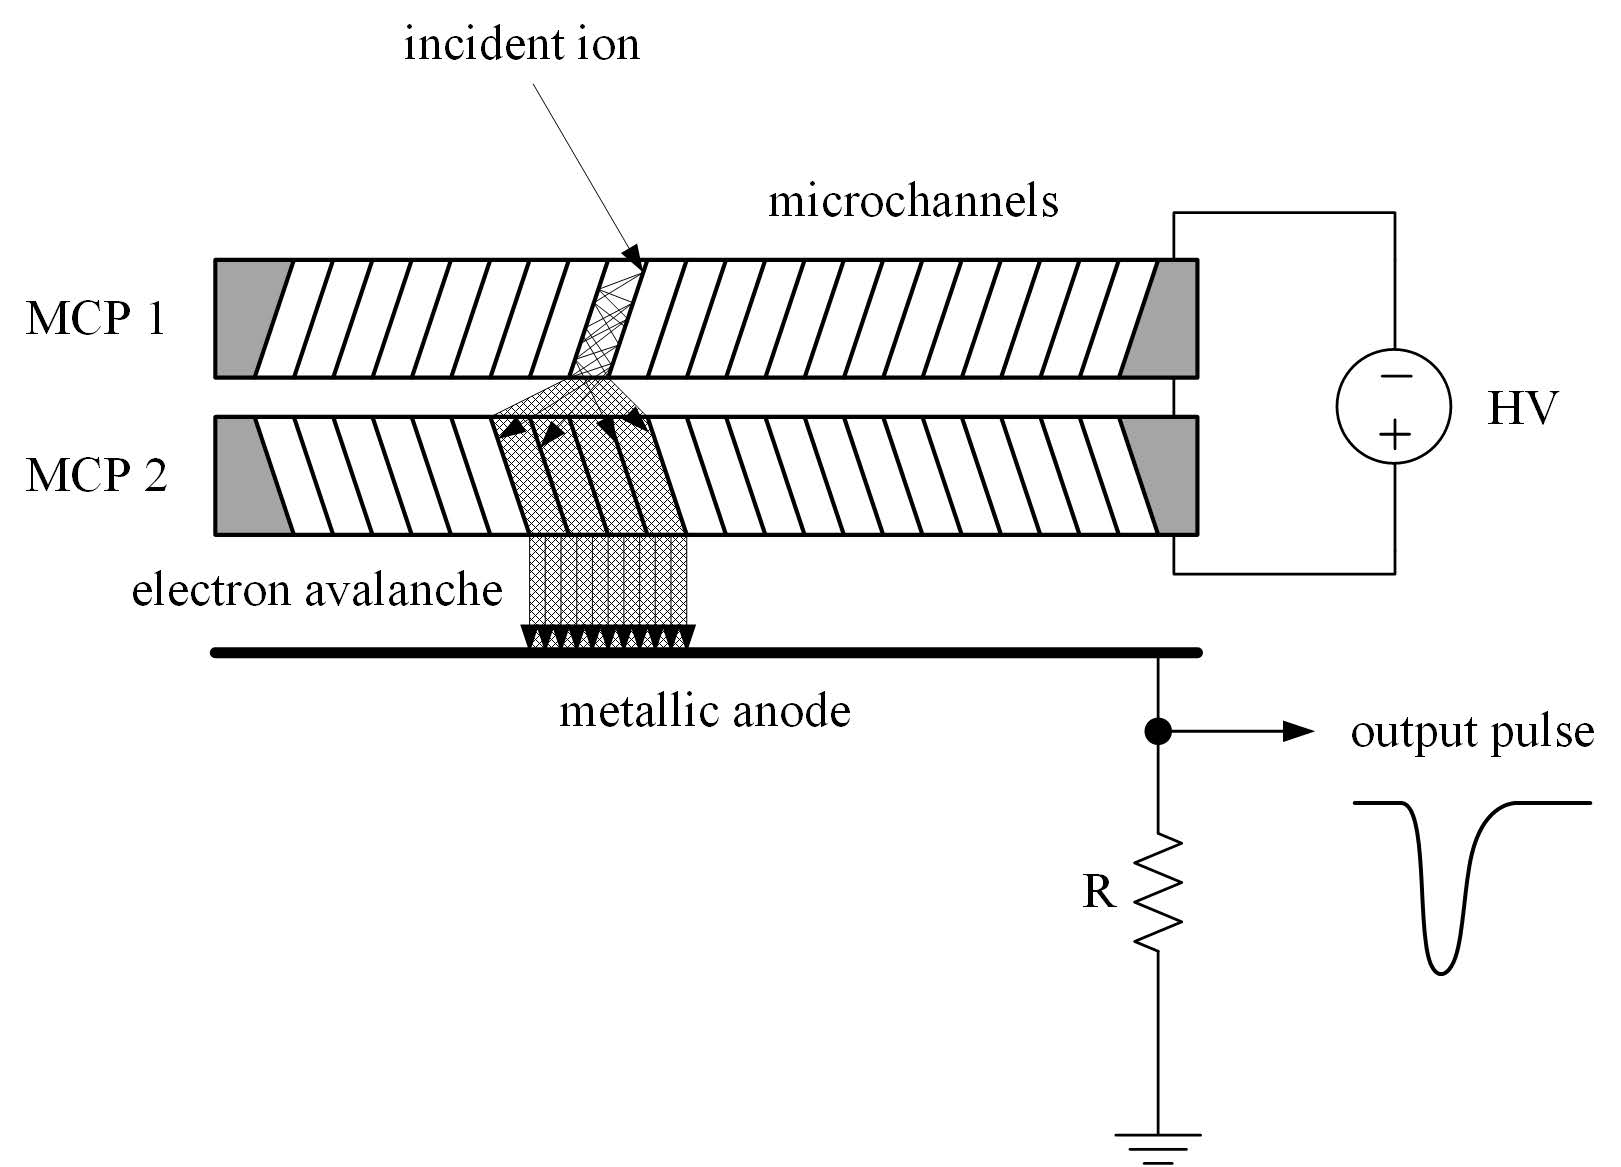
\includegraphics[width=.7\textwidth]{Bilder/MCP_PrinipleSchema.jpg}
		\caption{Working principle of a Multichannel Plates (MCPs) detector \cite{Wiza_1979_MCP,Diss_Meyer}.}
		\label{fig:MCPPrincipleSchema}
	\end{figure}
	
	\subsubsection{MCP Gain}\label{chap:MCPGain}
	In this section, the gain of a single MCP is derived as a function of the voltage $U_{MCP}$ applied over the MCP. The derivation is based on the lecture notes of \cite{LecNot_Wurz2017}. When an incoming particle hits the MCP channel wall there is a certain probability that it ejects an electron. By applying an electric field $E$ over the MCP plate, this electron gets accelerated along the channel axis until it hits the opposite wall, where it ejects more electrons (Fig.~\ref{fig:MCPPrincipleSchema}):
	\begin{equation}
		E = \frac{U_{MCP}}{l} = \frac{F}{q_0} = \frac{a m_e}{q_0}
	\end{equation}
	With $U_{MCP}$ the voltage applied over the MCP, $l$ the channel length, $F$ the force applied on the electron, $q_0$ the elementary charge and $m_e$ the mass of the electron. The acceleration $a$ of the electron along the channel is:		
	\begin{equation}
		a = \frac{U_{MCP}\cdot q_0}{l\cdot m_e}
	\end{equation}
	The distance $s$ the electron travels along the channel until it reaches the opposite channel wall is:
	\begin{equation}
		s = \frac{1}{2}at^2 = \frac{U_{MCP}\cdot q_0\cdot t^2}{l\cdot m_e\cdot 2}
		\label{eq:DetGainChFlightDist}
	\end{equation}
	With $t$ the flight time of the electron until it hits the wall again. Assuming the initial velocity $v_{init}$ of the initial secondary electron is perpendicular to the channel wall, the flight distance until it hits the opposite channel wall is the channel diameter $d$. The flight time $t$ can be written as:
	\begin{equation}
		t = \frac{d}{v_{init}}
		\label{eq:DetGainChFlightTime}
	\end{equation}
	$v_{init}$ is derived from the electron's initial kinetic energy $U_{init}$:
	\begin{equation}
		U_{init} = \frac{1}{2}m_e v_{init}^2 \rightarrow v_{init} = \sqrt{\frac{2U_{init}}{m_e}}
		\label{eq:DetGainEkin}
	\end{equation}
	where $U_{init}$ is the mean energy of a released electron (secondary electron) upon electron impact on the surface. By inserting Eq.~\eqref{eq:DetGainChFlightTime} and Eq.~\eqref{eq:DetGainEkin} in Eq.~\eqref{eq:DetGainChFlightDist} leads to:
	\begin{equation}
		s = \frac{q_0 \cdot U_{MCP}\cdot d^2}{l\cdot 4U_{init}}
		\label{eq:DetGainDistECh}
	\end{equation}
	The energy $U_c$ the electron gains during the flight time $t$ is:
	\begin{align}
		U_c =& q_0 Es = q_0\cdot \frac{U_{MCP}}{l}\cdot\frac{q_0\cdot U_{MCP}\cdot d^2}{l\cdot 4 U_{init}}\\
		=& q_0^2 \frac{U_{MCP}^2\cdot d^2}{l^2\cdot 4U_{init}}
	\end{align}
	The secondary electron emission coefficient $\delta$ is proportional to the square root of the energy $U_c$:
	\begin{equation}
		\delta = A\cdot \sqrt{U_c} = A\cdot \frac{q_0 U_{MCP}\cdot d}{2 \sqrt{U_{init}}\cdot l}
		\label{eq:DetGainDelta}
	\end{equation}
	With $A$ a constant containing the details of the interaction of the impinging electron with the electrons of the surface. After $n$ collisions with the channel walls, the gain $G_{ch}$ of one channel is:
	\begin{equation}
		G_{ch} = \gamma\cdot\delta^{n} = \gamma\cdot\delta^{l/s}
		\label{eq:detGainDel}
	\end{equation}
	With $\gamma$ containing the probability to emit the first electron upon ion impact. The number of collisions is the channel length $l$ divided by the distance $s$ an electron flies within the channel before it hits the channel wall and ejects more electrons. Inserting now Eq.~\eqref{eq:DetGainDelta} and Eq.~\eqref{eq:DetGainDistECh} in Eq.~\eqref{eq:detGainDel} leads to:
	\begin{equation}
		G_{ch} = \gamma\left(A\cdot\frac{q_0 U_{MCP}}{2\sqrt{U_{init}}}\cdot\frac{d}{l}\right) ^{\frac{4U_{init}}{q_0 U_{MCP}}\left(\frac{l}{d}\right)^2}
	\end{equation}
	By writing the channel length to diameter ratio $\frac{l}{d}$ as $\alpha$ and expressing the electrons initial energy $U_{init}$ in [eV], the equation turns into:
	\begin{equation}
		G_{ch} = \gamma\left(A\frac{U_{MCP}}{2\alpha\sqrt{U_{init}}}\right)^{\frac{4\cdot U_{init}\cdot\alpha^2}{U_{MCP}}}
		\label{eq:MCPGain}
	\end{equation}
	With $\gamma$ in the range of 0.1--10, $A$ approximately 0.2 $\left(\frac{1}{eV}\right)^{1/2}$ \cite{Wiza_1979_MCP}, $U_{MCP}$ in [eV], $\alpha$ is a dimensionless number, and $U_{init}$ in the range of a few [eV].
	
	
%-------------------------------------------------------------------------------------------	
	\subsubsection{Dead time}
	In this chapter, the dead time $\tau$ of the MCPs used in the NIM detector is derived. The dead time is the time one single channel of the MCP needs to replenish 63\% of its charge. After 5$\tau$ the channel is fully recharged. When the ion count rate is too high, an ion will hit the channel during the time the channel is recharging. The corresponding channel discharges and the triggered signal will be lower because the channel was not fully charged when the signal was triggered. Therefore, it is important to know the dead time to get an estimation of the upper limit of the count rate of the detector.\\
	\begin{figure}[H]
		\centering
		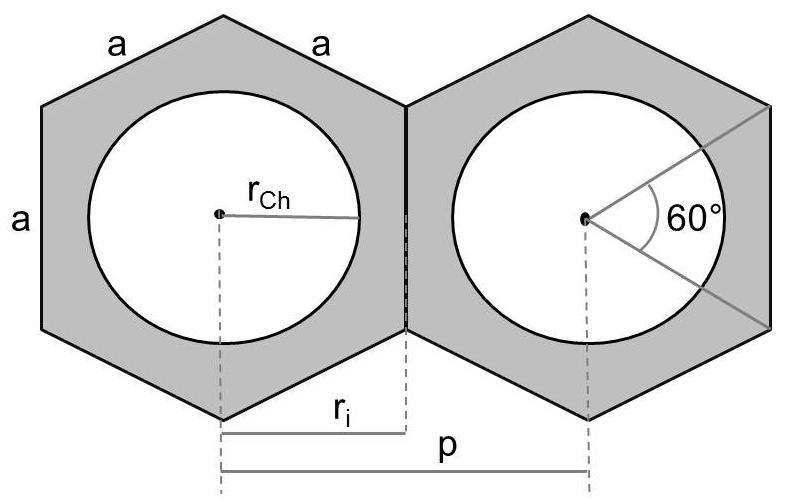
\includegraphics[width=.4\textwidth]{Bilder/MCP_hex.jpg}
		\caption{MCP honeycomb structure \cite{Diss_Neuland}.}
		\label{fig:MCPhex}
	\end{figure}
	The number of channels $N$ of a MCP is its active area $A_{act}$ divided by the area of one channel $A_{hex}$. The MCP has a honeycomb like structure (Fig.~\ref{fig:MCPhex}). Thus, the area of one channel is the area of a hexagon:
	\begin{equation}
		N = \frac{A_{act}}{A_{hex}} = \frac{2\cdot\pi r^2_{act}}{\sqrt{3}p^2}
	\end{equation}
	$r_{act}$ is the radius of the active area of the MCP, which is for the NIM MCPs 8~mm and $p$ is the distance between the centres of two channels which is 6~\si{\micro\meter}. This results in $1.6\cdot10^6$ channels of a NIM MCP. The resistance of a single channel is the resistance of the whole MCP plate $R_{MCP}$ times the number of channels $N$:
	\begin{equation}
		R_{ch} = R_{MCP}\cdot N
	\end{equation}
	The channel resistance depends on the voltage applied over the plate. For a nominal voltage of 1000~\si{\volt} $R_{MCP}$ is $\sim$70~\si{\mega\ohm} resulting in a channel resistance of about $10^{14}$~\si{\ohm}. The MCPs consist of two different materials: the structure (grey), which consists of a type of lead glass, and the hole, which is approximated with vacuum (white) (Fig.~\ref{fig:MCPhex}). The area of the structure is equal to the area of the hexagon $A^{hex}_{ch}$ minus the area of the channel hole $A^{hole}_{ch}$. The capacitance of one channel $C_{ch}$ is:
	\begin{equation}
		C_{ch} = \frac{\epsilon_0  (\epsilon_r \cdot (A^{hex}_{ch} - A^{hole}_{ch})+ A^{hole}_{ch})}{l_{ch}}
	\end{equation}
	With $\epsilon_0$ the vacuum permittivity, $\epsilon_r$ the relative permittivity of lead glass and $l_{ch}$ the MCP thickness which is 0.3~mm. The manufacturer does not give details about the material characteristics as it is a company secret. In \cite{Diss_Neuland} is an analysis of different values for $\epsilon_r$ found in literature. These values are between 6 and 20. With these values, the resulting capacity is 5~\si{\atto\farad} per channel. The dead time of a single MCP channel is the channel resistance $R_{ch}$ times the channel capacitance $C_{ch}$:
	\begin{equation}
		\tau = R_{ch}\cdot C_{ch}
	\end{equation}
	This results in a dead time of $\tau =$ 500~\si{\micro\second}. With a duration of about 100~\si{\micro\second} for the recording time of one waveform, this channel would be blind for the time when the next five waveforms are recorded. With $1.6\cdot10^6$ channels and assuming a uniform distribution of ions on the MCP surface, saturation is assumed at particle rates $I_p$ higher than $10^9$ particles/\si{\second}. The current drawn by the MCPs due to that high count rate is the particle count rate $I_p$ times the MCP gain $G$ and the elementary charge $q_0$
	\begin{equation}
		I_{MCP} = I_p\cdot G \cdot q_0
	\end{equation}
	resulting in a current of $\sim$100~\si{\micro\ampere}. The MCPs have a leakage current between 6--30~\si{\micro\ampere}. The additional current drawn by the NIM detector due to the amplification of the ions is lower than a few \si{\micro\ampere} resulting in two decades of margin before the detector reaches saturation.
	
	
	
	

	
	





	